\documentclass[12pt, a4paper, twoside]{report}

\usepackage{setspace}
\onehalfspacing
%\doublespacing
\usepackage{amsmath, amssymb, amsthm, mathtools,mathrsfs}
\usepackage{pifont}
\allowdisplaybreaks % to break align maths over pages
\usepackage[colorlinks=true, linkcolor=blue, citecolor=blue]{hyperref}
\usepackage{bbm, bm}
\usepackage{url}
\usepackage{fancyhdr} %, xspace, psfrag, setspace, supertabular
\usepackage{algorithm, algpseudocode}
\usepackage{graphicx}
\usepackage{geometry} % min OU requirements [inner=40mm, outer=15mm, top=15mm, bottom=20mm]
\usepackage[dvipsnames]{xcolor}
\usepackage{tikz}
\usetikzlibrary{automata,positioning,decorations.pathreplacing}
\tikzset{>=latex}
\usepackage[procnames]{listings} % Allows inclusion (and syntax highlighting) of C code blocks
\usepackage[font={small}]{caption}
\usepackage{subcaption}
\usepackage{footnote} 
\makesavenoteenv{tabular} % to be able to use footnotes in tabulars
\makesavenoteenv{table} % to be able to use footnotes in tables
\usepackage{stmaryrd} % for averaging operator
\usepackage[utf8]{inputenc}
\usepackage[T1]{fontenc}
\usepackage{mathdots}


\begin{document}




\newtheorem{theorem}{Theorem}[section]
\newtheorem{proposition}{Proposition}[section]
\newtheorem{corollary}{Corollary}[section]
\newtheorem{lemma}{Lemma}[section]
\theoremstyle{definition}
\newtheorem{definition}{Definition}[section]
\newtheorem{example}{Example}[section]
\newtheorem*{note}{Note}
\newtheorem{remark}{Remark}[section]
\newtheorem{observation}{Observation}[section]

\definecolor{keywords}{RGB}{255,0,90}
\definecolor{comments}{RGB}{0,0,113}
\definecolor{myred}{RGB}{160,0,0}
\definecolor{green}{RGB}{0,150,0}


%% For typesetting code listings                                                
\lstdefinelanguage{Sage}[]{Python}
{morekeywords={False,sage,True},sensitive=true}
\newcommand{\lstsetsage}{\lstset{
  frame=single,
  showtabs=False,
  showspaces=False,
  showstringspaces=False,
  commentstyle={\ttfamily\color{dgraycolor}},
  keywordstyle={\ttfamily\color{dbluecolor}\bfseries},
  stringstyle={\ttfamily\color{dgreencolor}\bfseries},
  language=Sage,
  basicstyle={\fontsize{9pt}{9pt}\ttfamily},
  aboveskip=0.3em,
  belowskip=0.1em,
  numbers=left,
  numberstyle=\tiny
}}

\newcommand{\lstsetbash}{\lstset{
    language=bash,
    basicstyle={\fontsize{9pt}{9pt}\ttfamily},
    deletekeywords={local, for, help},
    keywordstyle=\color{keywords},
    commentstyle=\color{comments},
    stringstyle=\color{black},
    numbers=none,
    stepnumber=1,
    frame=single,
    showstringspaces=false,
}}

\definecolor{dblackcolor}{rgb}{0.0,0.0,0.0}
\definecolor{dbluecolor}{rgb}{0.01,0.02,0.7}
\definecolor{dgreencolor}{rgb}{0.2,0.4,0.0}
\definecolor{dgraycolor}{rgb}{0.30,0.3,0.30}
\newcommand{\dblue}{\color{dbluecolor}\bf}
\newcommand{\dred}{\color{dredcolor}\bf}
\newcommand{\dblack}{\color{dblackcolor}\bf}


\newcommand{\shellcmd}[1]{\texttt{\footnotesize\$ #1}}
\renewcommand{\vert}[1]{\ensuremath{\llbracket #1 \rrbracket}} % Razborov's averaging operator
\newcommand{\Av}{\ensuremath{\mathrm{Av}}}
\newcommand{\Si}{\ensuremath{\mathrm{Si}}}
\newcommand{\seq}[1]{\text{\textsc{Seq}}[#1]}
\newcommand{\D}[1]{\ensuremath{\mathrm{\textbf{D}}}}
\renewcommand{\P}{\ensuremath{\mathcal{P}}}
\newcommand{\T}{\ensuremath{\mathcal{T}}}
\newcommand{\V}{\ensuremath{\mathcal{V}}}
\newcommand{\B}{\ensuremath{\mathcal{B}}}
\newcommand{\Z}{\ensuremath{\mathcal{Z}}}
\newcommand{\Zstar}{\ensuremath{\mathcal{Z}^*}}
\newcommand{\M}{\ensuremath{\mathcal{M}}}
\newcommand{\Mstar}{\ensuremath{\mathcal{M}^*}}
\newcommand{\barMstar}{\ensuremath{\overline{\mathcal{M}}^*}}
\newcommand{\EE}{\ensuremath{\mathcal{E}}}
\newcommand{\C}{\ensuremath{\mathcal{C}}}
\newcommand{\Cstar}{\ensuremath{\mathcal{C}^*}}
\newcommand{\HH}{\ensuremath{\mathcal{H}}}
\newcommand{\HHstar}{\ensuremath{\mathcal{H}^*}}
\newcommand{\hatC}{\ensuremath{\widehat{\mathcal{C}}}}
\newcommand{\hatCstar}{\ensuremath{\widehat{\mathcal{C}}^*}}
\newcommand{\barC}{\ensuremath{\overline{\mathcal{C}}}}
\newcommand{\barCstar}{\ensuremath{\overline{\mathcal{C}}^*}}
\newcommand{\Q}{\ensuremath{\mathcal{Q}}}
\newcommand{\F}{\ensuremath{\mathcal{F}}}
\renewcommand{\S}{\ensuremath{\mathcal{S}}}
\newcommand{\Sstar}{\ensuremath{\mathcal{S}^*}}
\renewcommand{\SS}{\ensuremath{\mathbb{S}}}
\newcommand{\rS}{\ensuremath{\mathscr{S}}}
\newcommand{\DD}{\ensuremath{\mathcal{D}}}
\newcommand{\DDstar}{\ensuremath{\mathcal{D}^*}}
\newcommand{\RR}{\ensuremath{\mathbb{R}}}

% Serif font
\newcommand{\fL}{\ensuremath{\mathsf{L}}}
\newcommand{\fR}{\ensuremath{\mathsf{R}}}
\newcommand{\fD}{\ensuremath{\mathsf{D}}}
\newcommand{\fU}{\ensuremath{\mathsf{U}}}
\newcommand{\fC}{\ensuremath{\mathsf{C}}}
\newcommand{\fB}{\ensuremath{\mathsf{B}}}
\newcommand{\fS}{\ensuremath{\mathsf{S}}}
\newcommand{\fM}{\ensuremath{\mathsf{M}}}
\newcommand{\fE}{\ensuremath{\mathsf{E}}}
\newcommand{\fX}{\ensuremath{\mathsf{X}}}

% bold Serif font
\newcommand{\bD}{\ensuremath{\textbf{\textsf{D}}}}
\newcommand{\bU}{\ensuremath{\textbf{\textsf{U}}}}
\newcommand{\bC}{\ensuremath{\textbf{\textsf{C}}}}
\newcommand{\bE}{\ensuremath{\textbf{\textsf{E}}}}
\newcommand{\bbU}{\ensuremath{\mathbb{U}}}
\newcommand{\bM}{\ensuremath{\textbf{\textsf{M}}}}
\renewcommand{\bm}{\ensuremath{\mathbf{m}}}
\newcommand{\bc}{\ensuremath{\mathbf{c}}}
\newcommand{\be}{\ensuremath{\mathbf{e}}}

\newcommand{\distav}[2]{\ensuremath{\mathbb{A}_{#1}(#2)}}
\newcommand{\N}{\ensuremath{\mathbb{N}}}
\newcommand{\rhs}{\ensuremath{\mathrm{RHS}}}
\newcommand{\lhs}{\ensuremath{\mathrm{LHS}}}
\newcommand{\argmax}[1]{\ensuremath{\mathrm{argmax}(#1)}}
\newcommand{\argmin}[1]{\ensuremath{\mathrm{argmin}(#1)}}
\newcommand{\Prob}[1]{\ensuremath{\mathbf{Pr}\left(#1\right)}}
\newcommand{\E}[1]{\ensuremath{\mathbf{E}\left(#1\right)}}
\newcommand{\Exp}[2]{\ensuremath{\mathbf{E}_{#1}\left(#2\right)}}
\newcommand{\1}[1]{\ensuremath{\mathbbm{1}_{#1}}}
\newcommand{\2}[2]{\ensuremath{\mathbbm{1}_{#1}\left(#2\right)}}
\newcommand{\Space}{\ensuremath{\mathcal{S}}}
\newcommand{\powerset}[1]{\ensuremath{\mathcal{P}\left(#1\right)}}
\newcommand{\mg}[1]{\ensuremath{\mathrm{mg}\left(#1\right)}}
\newcommand{\gr}[1]{\ensuremath{\mathrm{gr}\left(#1\right)}}
\newcommand{\ugr}[1]{\ensuremath{\overline{\mathrm{gr}}\left(#1\right)}}
\newcommand{\ex}{\ensuremath{\mathrm{ex}}}
\newcommand{\im}{\ensuremath{\mathrm{im}}}
\newcommand{\bigominus}{\ensuremath{\mathlarger{\mathlarger{\mathlarger{\ominus}}}}}
\newcommand{\x}{\ensuremath{\mathbf{x}}}
\newcommand{\Grid}{\ensuremath{\mathrm{Grid}}}


%%%%%%%%%%%%%%%%%%%%%%%%%%%%%%%%%%%%%%%%%
% DYCK PATHS
%%%%%%%%%%%%%%%%%%%%%%%%%%%%%%%%%%%%%%%%%


% drawing Dyck paths:
\newcommand\dyck[4]{
  % start point, size, Dyck word (size x 2 booleans)
  \fill[white]  (#1) rectangle +(#2,#2);
  \draw[help lines] (#1) grid +(#2,#2);
  %\draw[dashed] (#1) -- +(#2,#2);
  \coordinate (prev) at (#1);
  \foreach \dir in {#4}{
    \ifnum\dir=0
    \coordinate (dep) at (1,0);
    \else
    \coordinate (dep) at (0,1);
    \fi
    \draw[line width=2pt, color=#3, cap=round] (prev) -- ++(dep) coordinate (prev);
  };
}


% drawing Dyck paths without grid
\newcommand\pdyck[3]{
  % start point, size, Dyck word (size x 2 booleans)
  \coordinate (prev) at (#1);
  \foreach \dir in {#3}{
    \ifnum\dir=0
    \coordinate (dep) at (1,0);
    \else
    \coordinate (dep) at (0,1);
    \fi
    \draw[line width=2pt, color=#2, cap=round, style=dotted] (prev) -- ++(dep) coordinate (prev);
  };
}


%%%%%%%%%%%%%%%%%%%%%%%%%%%%%%%%%%%%%%%%%%
% CONSTRUCTIONS OF PERMUTONS
%%%%%%%%%%%%%%%%%%%%%%%%%%%%%%%%%%%%%%%%%%
\newcommand{\acbmax}{
  \begin{tikzpicture}[scale=0.5]
    \draw (0,1.7)--(1.3,3);
    \draw (1.3,1)--(2,1.7);
    \draw (2,0.7)--(2.3,1);
    \draw (2.3,0.5)--(2.5,0.7);
    \draw (2.5,0.4)--(2.6,0.5);
    \draw (2.65,0.3)--(2.7,0.35);
  \end{tikzpicture}}


\newcommand{\acdbmax}{
  \begin{tikzpicture}[scale=0.4]

    %\node at (-8,0) {$\Gamma\ = $};
    \draw (3,6)--(5,8);
    \draw (5,4.7)--(6.3,6);
    \draw (6.3,4)--(7,4.7);
    \draw (7,3.7)--(7.3,4);
    \draw (7.3,3.5)--(7.5,3.7);
    \draw (7.5,3.4)--(7.6,3.5);
    \draw (7.65,3.3)--(7.7,3.35);

    \draw (0,1.7)--(1.3,3);
    \draw (1.3,1)--(2,1.7);
    \draw (2,0.7)--(2.3,1);
    \draw (2.3,0.5)--(2.5,0.7);
    \draw (2.5,0.4)--(2.6,0.5);
    \draw (2.65,0.3)--(2.7,0.35);

    \draw (-1.7,-0.7)--(-1,0);
    \draw (-1,-1)--(-0.7,-0.7);
    \draw (-0.7,-1.2)--(-0.5,-1);
    \draw (-0.5,-1.3)--(-0.4,-1.2);
    \draw (-0.35,-1.4)--(-0.3,-1.35);

    \draw (-2.7,-2.3)--(-2.4,-2);
    \draw (-2.4,-2.5)--(-2.2,-2.3);
    \draw (-2.2,-2.6)--(-2.1,-2.5);
    \draw (-2.05,-2.7)--(-2,-2.65);

    \draw[thick] (-3.05,-3.05)--(-3,-3);
    \draw[thick] (-3.25,-3.25)--(-3.2,-3.2);
    \draw[thick] (-3.45,-3.45)--(-3.4,-3.4);


    \draw (14,2)--(16,2);
    \draw (14,1.5)--(16,1.5);

    \draw (25,6)--(27,8)--(29.7,3.35)--(25,6);
    \draw (20,-2.35)--(25,-2.35)--(25,3.35)--(20,3.35)--(20,-2.35);

  \end{tikzpicture}}






\newcommand{\Amax}{
  \begin{tikzpicture}[baseline=1ex, scale=0.15]
    \draw (0,1.7)--(1.3,3);
    \draw (1.3,1)--(2,1.7);
    \draw (2,0.7)--(2.3,1);
    \draw (2.3,0.5)--(2.5,0.7);
    \draw (2.5,0.4)--(2.6,0.5);
    \draw (2.65,0.3)--(2.7,0.35);

    \draw (3,5)--(5,3);
  \end{tikzpicture}}

\newcommand{\AAmax}{
  \begin{tikzpicture}[baseline=1ex, scale=0.15]
    \draw (0,1.7)--(1.3,3);
    \draw (1.3,1)--(2,1.7);
    \draw (2,0.7)--(2.3,1);
    \draw (2.3,0.5)--(2.5,0.7);
    \draw (2.5,0.4)--(2.6,0.5);
    \draw (2.65,0.3)--(2.7,0.35);

    \draw (2.5,5)--(5,2.5);
  \end{tikzpicture}}




\newcommand{\Bmax}{
  \begin{tikzpicture}[baseline=1ex, scale=0.15]
    \draw (3,3)--(5,5);
    \draw (5,1)--(7,3);

    \draw (1,0)--(2,1);
    \draw (2,-1)--(3,0);
    
    \draw (0,-1.5)--(0.5,-1);
    \draw (0.5,-2)--(1,-1.5);

    \draw (-0.4,-2.2)--(-0.2,-2);
    \draw (-0.2,-2.4)--(0,-2.2);

  \end{tikzpicture}}



\newcommand{\Cmax}{
  \begin{tikzpicture}[baseline=1ex, scale=0.15]

    \draw (3,5)--(5,3);
    \draw (2,3)--(3,2);
    \draw (1,2)--(2,1);
    \draw (-1,1)--(1,-1);
  \end{tikzpicture}}




\newcommand{\Dmax}{
  \begin{tikzpicture}[baseline=1ex, scale=0.15]
    \draw (0,1.7)--(1.3,3);
    \draw (1.3,1)--(2,1.7);
    \draw (2,0.7)--(2.3,1);
    \draw (2.3,0.5)--(2.5,0.7);
    \draw (2.5,0.4)--(2.6,0.5);
    \draw (2.65,0.3)--(2.7,0.35);

    \draw (3,4.7)--(4.3,6);
    \draw (4.3,4)--(5,4.7);
    \draw (5,3.7)--(5.3,4);
    \draw (5.3,3.5)--(5.5,3.7);
    \draw (5.5,3.4)--(5.6,3.5);
    \draw (5.65,3.3)--(5.7,3.35);
  \end{tikzpicture}}

\newcommand{\Dmaxr}{
  \begin{tikzpicture}[baseline=1ex, scale=0.15]
    \draw (0,1.7)--(1.3,3);
    \draw (1.3,1)--(2,1.7);
    \draw (2,0.7)--(2.3,1);
    \draw (2.3,0.5)--(2.5,0.7);
    \draw (2.5,0.4)--(2.6,0.5);
    \draw (2.65,0.3)--(2.7,0.35);

    \draw (4.5,3)--(5.8,4.3);
    \draw (3.8,4.3)--(4.5,5);
    \draw (3.5,5)--(3.8,5.3);
    \draw (3.3,5.3)--(3.5,5.5);
    \draw (3.2, 5.5)--(3.3, 5.6);
    \draw (3.15, 5.6)--(3.2, 5.65);
  \end{tikzpicture}}


\newcommand{\Emax}{
  \begin{tikzpicture}[baseline=1ex, scale=0.15]

    \draw (0,2)--(2,0);
    \draw (2,4)--(4,6);
    \draw (4,2)--(6,4);
  \end{tikzpicture}}



% 1342 7term
\newcommand{\acdbmaxapprox}{
  \begin{tikzpicture}[baseline=1ex, scale=0.5]
    \draw (0,1.7)--(1.3,3);
    \draw (1.3,1)--(2,1.7);
    \draw (2,0.7)--(2.3,1);
    \draw (2.3,0.5)--(2.5,0.7);
    \draw (2.5,0.4)--(2.6,0.5);
    \draw (2.65,0.3)--(2.7,0.35);
  \end{tikzpicture}}


%%%%%%%%%%%%%%%%%%%%%%%%%%%%%%%%%%%%%%%%%%%%
% SMALL PERMUTATION PICTOGRAMS
%%%%%%%%%%%%%%%%%%%%%%%%%%%%%%%%%%%%%%%%%%%%

\newcommand{\dicycle}{
  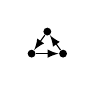
\begin{tikzpicture}[baseline=-0.3ex,scale=0.2]
    \tikzstyle{vertex}=[circle,fill=black, minimum size=1pt,inner sep=1pt]
    \node[vertex] (v1) at (0,0){};
    \node[vertex] (v2) at (2,0){};
    \node[vertex] (v3) at (1,1.4){};
    \draw[->](v1)--(v2);
    \draw[->](v2)--(v3);
    \draw[->](v3)--(v1);
  \end{tikzpicture}
}

\newcommand{\twochain}{
  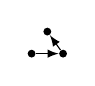
\begin{tikzpicture}[baseline=-0.3ex,scale=0.2]
    \tikzstyle{vertex}=[circle,fill=black, minimum size=1pt,inner sep=1pt]
    \node[vertex] (v1) at (0,0){};
    \node[vertex] (v2) at (2,0){};
    \node[vertex] (v3) at (1,1.4){};
    \draw[->](v1)--(v2);
    \draw[->](v2)--(v3);
  \end{tikzpicture}
}

\newcommand{\orcocherry}{
  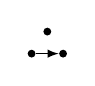
\begin{tikzpicture}[baseline=-0.3ex,scale=0.2]
    \tikzstyle{vertex}=[circle,fill=black, minimum size=1pt,inner sep=1pt]
    \node[vertex] (v1) at (0,0){};
    \node[vertex] (v2) at (2,0){};
    \node[vertex] (v3) at (1,1.4){};
    \draw[->](v1)--(v2);
  \end{tikzpicture}
}

\newcommand{\outstar}{
  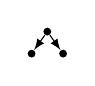
\begin{tikzpicture}[baseline=-0.3ex,scale=0.2]
    \tikzstyle{vertex}=[circle,fill=black, minimum size=1pt,inner sep=1pt]
    \node[vertex] (v1) at (0,0){};
    \node[vertex] (v2) at (2,0){};
    \node[vertex] (v3) at (1,1.4){};
    \draw[->](v3)--(v1);
    \draw[->](v3)--(v2);
  \end{tikzpicture}
}


\newcommand{\digraphacbd}{
  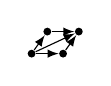
\begin{tikzpicture}[baseline=-0.3ex,scale=0.2]
    \tikzstyle{vertex}=[circle,fill=black, minimum size=1pt,inner sep=1pt]
    \node[vertex] (v1) at (0,0){};
    \node[vertex] (v2) at (2,0){};
    \node[vertex] (v3) at (1,1.4){};
    \node[vertex] (v4) at (3, 1.4){};
    \draw[->](v1)--(v2);
    \draw[->](v1)--(v3);
    \draw[->](v1)--(v4);
    \draw[->](v2)--(v4);
    \draw[->](v3)--(v4);
  \end{tikzpicture}
}

%\input struct.tex
\newcommand{\gridbadc}{
  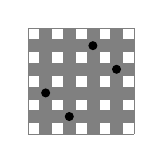
\begin{tikzpicture}[baseline=0.5ex,scale=0.15]
  \tikzstyle{vertex}=[circle,draw=black, fill=black, minimum size=2pt,inner sep=1pt]

  \draw[gray, very thin] (0,0) grid (9,9);
  \fill[gray] (1,0) rectangle (2,9);
  \fill[gray] (3,0) rectangle (4,9);
  \fill[gray] (5,0) rectangle (6,9);
  \fill[gray] (7,0) rectangle (8,9);

  \fill[gray] (0,1) rectangle (9,2);
  \fill[gray] (0,3) rectangle (9,4);
  \fill[gray] (0,5) rectangle (9,6);
  \fill[gray] (0,7) rectangle (9,8);
  
  \node[vertex] (v1) at (1.5, 3.5){};
  \node[vertex] (v2) at (3.5,1.5){};
  \node[vertex] (v3) at (5.5,7.5){};
  \node[vertex] (v4) at (7.5,5.5){};
  \draw (v1) (v2) (v3) (v4);
  \end{tikzpicture}}



\newcommand{\gridabdc}{
  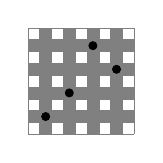
\begin{tikzpicture}[baseline=0.5ex,scale=0.15]
  \tikzstyle{vertex}=[circle,draw=black, fill=black, minimum size=2pt,inner sep=1pt]

  \draw[gray, very thin] (0,0) grid (9,9);
  \fill[gray] (1,0) rectangle (2,9);
  \fill[gray] (3,0) rectangle (4,9);
  \fill[gray] (5,0) rectangle (6,9);
  \fill[gray] (7,0) rectangle (8,9);

  \fill[gray] (0,1) rectangle (9,2);
  \fill[gray] (0,3) rectangle (9,4);
  \fill[gray] (0,5) rectangle (9,6);
  \fill[gray] (0,7) rectangle (9,8);
  
  \node[vertex] (v1) at (1.5, 1.5){};
  \node[vertex] (v2) at (3.5,3.5){};
  \node[vertex] (v3) at (5.5,7.5){};
  \node[vertex] (v4) at (7.5,5.5){};
  \draw (v1) (v2) (v3) (v4);
  \end{tikzpicture}}



\newcommand{\gridbacd}{
  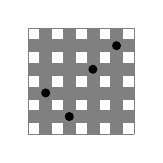
\begin{tikzpicture}[baseline=0.5ex,scale=0.15]
  \tikzstyle{vertex}=[circle,draw=black, fill=black, minimum size=2pt,inner sep=1pt]

  \draw[gray, very thin] (0,0) grid (9,9);
  \fill[gray] (1,0) rectangle (2,9);
  \fill[gray] (3,0) rectangle (4,9);
  \fill[gray] (5,0) rectangle (6,9);
  \fill[gray] (7,0) rectangle (8,9);

  \fill[gray] (0,1) rectangle (9,2);
  \fill[gray] (0,3) rectangle (9,4);
  \fill[gray] (0,5) rectangle (9,6);
  \fill[gray] (0,7) rectangle (9,8);
  
  \node[vertex] (v1) at (1.5, 3.5){};
  \node[vertex] (v2) at (3.5,1.5){};
  \node[vertex] (v3) at (5.5,5.5){};
  \node[vertex] (v4) at (7.5,7.5){};
  \draw (v1) (v2) (v3) (v4);
  \end{tikzpicture}}




%%%%%%%%%%%%%%%%%%%%%%%%%%%%%%%%%%%%%%%%%%%%%%%%%%%%%%%%%%%%%%%%%%%%%%%%%%%%%%%%%%%
% 1-POINT PERMTUATIONS
%%%%%%%%%%%%%%%%%%%%%%%%%%%%%%%%%%%%%%%%%%%%%%%%%%%%%%%%%%%%%%%%%%%%%%%%%%%%%%%%%%%



\newcommand{\atau}{
  \begin{tikzpicture}[baseline=0.5ex,scale=0.15]
  \tikzstyle{vertex}=[circle,draw=black,fill=white, minimum size=2pt,inner sep=1pt]
  \node[vertex] (v1) at (0.5, 0.5){};
  \draw (v1);
  \end{tikzpicture}}

\renewcommand{\a}{
  \begin{tikzpicture}[baseline=0.5ex,scale=0.15]
  \tikzstyle{vertex}=[circle,fill=black, minimum size=2pt,inner sep=1pt]
  \node[vertex] (v1) at (0.5, 0.5){};
  \draw (v1);
  \end{tikzpicture}}


%%%%%%%%%%%%%%%%%%%%%%%%%%%%%%%%%%%%%%%%%%%%%%%%%%%%%%%%%%%%%%%%%%%%%%%%%%%%%%%%%%%
% 2-POINT PERMTUATIONS
%%%%%%%%%%%%%%%%%%%%%%%%%%%%%%%%%%%%%%%%%%%%%%%%%%%%%%%%%%%%%%%%%%%%%%%%%%%%%%%%%%%

\newcommand{\abtau}{
  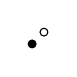
\begin{tikzpicture}[baseline=0.5ex,scale=0.15]
  \tikzstyle{vertex}=[circle,draw=black, fill=black, minimum size=2pt,inner sep=1pt]
  \node[vertex] (v1) at (0.5, 0.5){};
  \tikzstyle{vertex}=[circle,draw=black, fill=white, minimum size=2pt,inner sep=1pt]
  \node[vertex] (v2) at (1.5,1.5){};
  %\draw[gray, very thin] (0,0) grid (2,2);
  \draw (v1) (v2);
  \end{tikzpicture}}

\newcommand{\tauab}{
  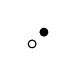
\begin{tikzpicture}[baseline=0.5ex,scale=0.15]
  \tikzstyle{vertex}=[circle,draw=black, fill=white, minimum size=2pt,inner sep=1pt]
  \node[vertex] (v1) at (0.5, 0.5){};
  \tikzstyle{vertex}=[circle,draw=black, fill=black, minimum size=2pt,inner sep=1pt]
  \node[vertex] (v2) at (1.5,1.5){};
  %\draw[gray, very thin] (0,0) grid (2,2);
  \draw (v1) (v2);
  \end{tikzpicture}}

\newcommand{\tauba}{
  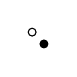
\begin{tikzpicture}[baseline=0.5ex,scale=0.15]
  \tikzstyle{vertex}=[circle, draw=black, fill=white, minimum size=2pt,inner sep=1pt]
  \node[vertex] (v1) at (0.5, 1.5){};
  \tikzstyle{vertex}=[circle, draw=black, fill=black, minimum size=2pt,inner sep=1pt]
  \node[vertex] (v2) at (1.5, 0.5){};
  %\draw[gray, very thin] (0,0) grid (2,2);
  \draw (v1) (v2);
  \end{tikzpicture}}

\newcommand{\batau}{
  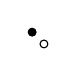
\begin{tikzpicture}[baseline=0.5ex,scale=0.15]
  \tikzstyle{vertex}=[circle, draw=black, fill=black, minimum size=2pt,inner sep=1pt]
  \node[vertex] (v1) at (0.5, 1.5){};
  \tikzstyle{vertex}=[circle, draw=black, fill=white, minimum size=2pt,inner sep=1pt]
  \node[vertex] (v2) at (1.5, 0.5){};
  %\draw[gray, very thin] (0,0) grid (2,2);
  \draw (v1) (v2);
  \end{tikzpicture}}


%================ PLAIN ================

\newcommand{\ab}{
  
\begin{tikzpicture}[baseline=0.5ex,scale=0.15]
  \tikzstyle{vertex}=[circle,fill=black, minimum size=2pt,inner sep=1pt]
  \node[vertex] (v1) at (0.5, 0.5){};
  \tikzstyle{vertex}=[circle,fill=black, minimum size=2pt,inner sep=1pt]
  \node[vertex] (v2) at (1.5,1.5){};
  %\draw[gray, very thin] (0,0) grid (2,2);
  \draw (v1) (v2);
  \end{tikzpicture}}

\newcommand{\ba}{
  
\begin{tikzpicture}[baseline=0.5ex,scale=0.15]
  \tikzstyle{vertex}=[circle, fill=black, minimum size=2pt,inner sep=1pt]
  \node[vertex] (v1) at (1.5, 1.5){};
  \tikzstyle{vertex}=[circle, fill=black, minimum size=2pt,inner sep=1pt]
  \node[vertex] (v2) at (0.5, 0.5){};
  %\draw[gray, very thin] (0,0) grid (2,2);
  \draw (v1) (v2);
  \end{tikzpicture}}



%%%%%%%%%%%%%%%%%%%%%%%%%%%%%%%%%%%%%%%%%%%%%%%%%%%%%%%%%%%%%%%%%%%%%%%%%%%%%%%%%%%
% 3-POINT PERMTUATIONS
%%%%%%%%%%%%%%%%%%%%%%%%%%%%%%%%%%%%%%%%%%%%%%%%%%%%%%%%%%%%%%%%%%%%%%%%%%%%%%%%%%%

\newcommand{\tauabc}{
  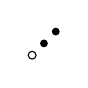
\begin{tikzpicture}[baseline=0.5ex,scale=0.15]
  \tikzstyle{vertex}=[circle,draw=black,fill=white, minimum size=2pt,inner sep=1pt]
  \node[vertex] (v1) at (0.5, 0.5){};
  \tikzstyle{vertex}=[circle,fill=black, minimum size=2pt,inner sep=1pt]
  \node[vertex] (v2) at (1.5,1.5){};
  \node[vertex] (v3) at (2.5, 2.5){};
  \draw (v1) (v2) (v3);
  \end{tikzpicture}}

\newcommand{\ataubc}{
  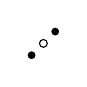
\begin{tikzpicture}[baseline=0.5ex,scale=0.15]
  \tikzstyle{vertex}=[circle,draw=black,fill=white, minimum size=2pt,inner sep=1pt]
  \node[vertex] (v1) at (1.5, 1.5){};
  \tikzstyle{vertex}=[circle,fill=black, minimum size=2pt,inner sep=1pt]
  \node[vertex] (v2) at (0.5,0.5){};
  \node[vertex] (v3) at (2.5, 2.5){};
  \draw (v1) (v2) (v3);
  \end{tikzpicture}}

\newcommand{\acbtau}{
  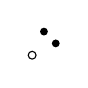
\begin{tikzpicture}[baseline=0.5ex,scale=0.15]
  \tikzstyle{vertex}=[circle,draw=black,fill=white, minimum size=2pt,inner sep=1pt]
  \node[vertex] (v1) at (0.5, 0.5){};
  \tikzstyle{vertex}=[circle,fill=black, minimum size=2pt,inner sep=1pt]
  \node[vertex] (v2) at (1.5,2.5){};
  \node[vertex] (v3) at (2.5, 1.5){};
  \draw (v1) (v2) (v3);
  \end{tikzpicture}}


\newcommand{\abc}{
  
\begin{tikzpicture}[baseline=0.5ex,scale=0.15]
  \tikzstyle{vertex}=[circle,fill=black, minimum size=2pt,inner sep=1pt]
  \node[vertex] (v1) at (0.5, 0.5){};
  \node[vertex] (v2) at (1.5,1.5){};
  \node[vertex] (v3) at (2.5, 2.5){};
  \draw (v1) (v2) (v3);
  \end{tikzpicture}}


\newcommand{\acb}{
  
\begin{tikzpicture}[baseline=0.5ex,scale=0.15]
  \tikzstyle{vertex}=[circle,fill=black, minimum size=2pt,inner sep=1pt]
  \node[vertex] (v1) at (0.5, 0.5){};
  \node[vertex] (v2) at (1.5,2.5){};
  \node[vertex] (v3) at (2.5, 1.5){};
  \draw (v1) (v2) (v3);
  \end{tikzpicture}}


\newcommand{\bac}{
  
\begin{tikzpicture}[baseline=0.5ex,scale=0.15]
  \tikzstyle{vertex}=[circle,fill=black, minimum size=2pt,inner sep=1pt]
  \node[vertex] (v2) at (0.5,1.5){};
  \node[vertex] (v1) at (1.5, 0.5){};
  \node[vertex] (v3) at (2.5, 2.5){};
  \draw (v1) (v2) (v3);
  \end{tikzpicture}}

\newcommand{\bca}{
  
\begin{tikzpicture}[baseline=0.5ex,scale=0.15]
  \tikzstyle{vertex}=[circle,fill=black, minimum size=2pt,inner sep=1pt]
  \node[vertex] (v1) at (0.5, 1.5){};
  \node[vertex] (v2) at (1.5,2.5){};
  \node[vertex] (v3) at (2.5, 0.5){};
  \draw (v1) (v2) (v3);
  \end{tikzpicture}}


\newcommand{\cba}{
  
\begin{tikzpicture}[baseline=0.5ex,scale=0.15]
  \tikzstyle{vertex}=[circle,fill=black, minimum size=2pt,inner sep=1pt]
  \node[vertex] (v3) at (0.5, 2.5){};
  \node[vertex] (v2) at (1.5,1.5){};
  \node[vertex] (v1) at (2.5, 0.5){};
  \draw (v1) (v2) (v3);
  \end{tikzpicture}}

\newcommand{\cab}{
  
\begin{tikzpicture}[baseline=0.5ex,scale=0.15]
  \tikzstyle{vertex}=[circle,fill=black, minimum size=2pt,inner sep=1pt]
  \node[vertex] (v1) at (0.5, 2.5){};
  \node[vertex] (v2) at (1.5,0.5){};
  \node[vertex] (v3) at (2.5, 1.5){};
  \draw (v1) (v2) (v3);
  \end{tikzpicture}}

%%%%%%%%%%%%%%%%%%%%%%%%%%%%%%%%%%%%%%%%%%%%%%%%%%%%%%%%%%%%%%%%%%%%%%%%%%%%%%%%%%%
% 4-POINT PERMTUATIONS
%%%%%%%%%%%%%%%%%%%%%%%%%%%%%%%%%%%%%%%%%%%%%%%%%%%%%%%%%%%%%%%%%%%%%%%%%%%%%%%%%%%

\newcommand{\abcd}{
  
\begin{tikzpicture}[baseline=0.6ex,scale=0.1]
  \tikzstyle{vertex}=[circle,fill=black, minimum size=2pt,inner sep=1pt]
  \node[vertex] (v1) at (0.5, 0.5){};
  \node[vertex] (v2) at (1.5, 1.5){};
  \node[vertex] (v3) at (2.5, 2.5){};
  \node[vertex] (v4) at (3.5, 3.5){};
  \draw (v1) (v2) (v3) (v4);
  \end{tikzpicture}}

\newcommand{\bdca}{
  
\begin{tikzpicture}[baseline=0.6ex,scale=0.1]
  \tikzstyle{vertex}=[circle,fill=black, minimum size=2pt,inner sep=1pt]
  \node[vertex] (v1) at (0.5, 1.5){};
  \node[vertex] (v2) at (1.5, 3.5){};
  \node[vertex] (v3) at (2.5, 2.5){};
  \node[vertex] (v4) at (3.5, 0.5){};
  \draw (v1) (v2) (v3) (v4);
  \end{tikzpicture}}

\newcommand{\acdb}{
  
\begin{tikzpicture}[baseline=0.6ex,scale=0.1]
  \tikzstyle{vertex}=[circle,fill=black, minimum size=2pt,inner sep=1pt]
  \node[vertex] (v1) at (0.5, 0.5){};
  \node[vertex] (v2) at (1.5, 2.5){};
  \node[vertex] (v3) at (2.5, 3.5){};
  \node[vertex] (v4) at (3.5, 1.5){};
  \draw (v1) (v2) (v3) (v4);
  \end{tikzpicture}}

%%%%%%%%%%%%%%%%%%%%%%%%%%%%%%%%%%%%%%%%%%%%%%%%%%%%%%%%%%%%%%%%%%%%%%%%%%%%%%%%%%%
% 5-POINT PERMTUATIONS
%%%%%%%%%%%%%%%%%%%%%%%%%%%%%%%%%%%%%%%%%%%%%%%%%%%%%%%%%%%%%%%%%%%%%%%%%%%%%%%%%%%

\newcommand{\bcaoba}{
  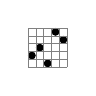
\begin{tikzpicture}[baseline=0.6ex,scale=0.1]
  \tikzstyle{vertex}=[circle,fill=black, minimum size=2pt,inner sep=1pt]
  \node[vertex] (v1) at (0.5, 1.5){};
  \node[vertex] (v2) at (1.5, 2.5){};
  \node[vertex] (v3) at (2.5, 0.5){};
  \node[vertex] (v4) at (3.5, 4.5){};
  \node[vertex] (v5) at (4.5, 3.5){};
  \draw[gray, very thin] (0,0) grid (5,5);
  \draw (v1) (v2) (v3) (v4) (v5);
  \end{tikzpicture}}


\newcommand{\baoaoba}{
  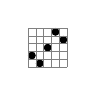
\begin{tikzpicture}[baseline=0.6ex,scale=0.1]
  \tikzstyle{vertex}=[circle,fill=black, minimum size=2pt,inner sep=1pt]
  \node[vertex] (v1) at (0.5, 1.5){};
  \node[vertex] (v2) at (1.5, 0.5){};
  \node[vertex] (v3) at (2.5, 2.5){};
  \node[vertex] (v4) at (3.5, 4.5){};
  \node[vertex] (v5) at (4.5, 3.5){};
  \draw[gray, very thin] (0,0) grid (5,5);
  \draw (v1) (v2) (v3) (v4) (v5);
  \end{tikzpicture}}


\newcommand{\aobamba}{
  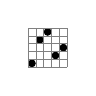
\begin{tikzpicture}[baseline=0.6ex,scale=0.1]
  \tikzstyle{vertex}=[circle,fill=black, minimum size=2pt,inner sep=1pt]
  \node[vertex] (v1) at (0.5, 0.5){};
  \node[vertex] (v2) at (1.5, 3.5){};
  \node[vertex] (v3) at (2.5, 4.5){};
  \node[vertex] (v4) at (3.5, 1.5){};
  \node[vertex] (v5) at (4.5, 2.5){};
  \draw[gray, very thin] (0,0) grid (5,5);
  \draw (v1) (v2) (v3) (v4) (v5);
  \end{tikzpicture}}



%%%%%%%%%%%%%%%%%%%%%%%%%%%%%%%%%%%%%%%%%%%%%%%%%%%%%%%%%%%%%%%%%%%%%%%%%%%%%%%%%%%
% 6-POINT PERMTUATIONS
%%%%%%%%%%%%%%%%%%%%%%%%%%%%%%%%%%%%%%%%%%%%%%%%%%%%%%%%%%%%%%%%%%%%%%%%%%%%%%%%%%%


\newcommand{\bcaocba}{
  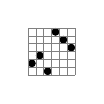
\begin{tikzpicture}[baseline=0.6ex,scale=0.1]
  \tikzstyle{vertex}=[circle,fill=black, minimum size=2pt,inner sep=1pt]
  \node[vertex] (v1) at (0.5, 1.5){};
  \node[vertex] (v2) at (1.5, 2.5){};
  \node[vertex] (v3) at (2.5, 0.5){};
  \node[vertex] (v4) at (3.5, 5.5){};
  \node[vertex] (v5) at (4.5, 4.5){};
  \node[vertex] (v6) at (5.5, 3.5){};
  \draw[gray, very thin] (0,0) grid (6,6);
  \draw (v1) (v2) (v3) (v4) (v5) (v6);
  \end{tikzpicture}}


\newcommand{\bcaobca}{
  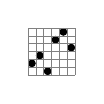
\begin{tikzpicture}[baseline=0.6ex,scale=0.1]
  \tikzstyle{vertex}=[circle,fill=black, minimum size=2pt,inner sep=1pt]
  \node[vertex] (v1) at (0.5, 1.5){};
  \node[vertex] (v2) at (1.5, 2.5){};
  \node[vertex] (v3) at (2.5, 0.5){};
  \node[vertex] (v4) at (3.5, 4.5){};
  \node[vertex] (v5) at (4.5, 5.5){};
  \node[vertex] (v6) at (5.5, 3.5){};
  \draw[gray, very thin] (0,0) grid (6,6);
  \draw (v1) (v2) (v3) (v4) (v5) (v6);
  \end{tikzpicture}}

\newcommand{\bcaocab}{
  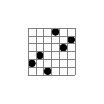
\begin{tikzpicture}[baseline=0.6ex,scale=0.1]
  \tikzstyle{vertex}=[circle,fill=black, minimum size=2pt,inner sep=1pt]
  \node[vertex] (v1) at (0.5, 1.5){};
  \node[vertex] (v2) at (1.5, 2.5){};
  \node[vertex] (v3) at (2.5, 0.5){};
  \node[vertex] (v4) at (3.5, 5.5){};
  \node[vertex] (v5) at (4.5, 3.5){};
  \node[vertex] (v6) at (5.5, 4.5){};
  \draw[gray, very thin] (0,0) grid (6,6);
  \draw (v1) (v2) (v3) (v4) (v5) (v6);
  \end{tikzpicture}}


\newcommand{\baoabmab}{
  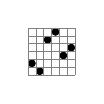
\begin{tikzpicture}[baseline=0.6ex,scale=0.1]
  \tikzstyle{vertex}=[circle,fill=black, minimum size=2pt,inner sep=1pt]
  \node[vertex] (v1) at (0.5, 1.5){};
  \node[vertex] (v2) at (1.5, 0.5){};
  \node[vertex] (v3) at (2.5, 4.5){};
  \node[vertex] (v4) at (3.5, 5.5){};
  \node[vertex] (v5) at (4.5, 2.5){};
  \node[vertex] (v6) at (5.5, 3.5){};
  \draw[gray, very thin] (0,0) grid (6,6);
  \draw (v1) (v2) (v3) (v4) (v5) (v6);
  \end{tikzpicture}}





%%%%%%%%%%%%%%%%%%%%%%%%%%%%%%%%%%%%%%%%%%%%%%%%%%%%%%%%%
%% GRID CLASSES
%%%%%%%%%%%%%%%%%%%%%%%%%%%%%%%%%%%%%%%%%%%%%%%%%%%%%%%%%

\newcommand{\cplusc}[2]{
  \begin{tikzpicture}[baseline=4ex, scale=0.8]
     % \filldraw[black] (0,2) circle (2pt);
      %\draw (-0.3,2.2) node {$\Z$};
      % \draw[-, very thick] (0.2,2.5) -- (0.2,0);
      % \draw[dashed] (0.2,2) -- (2.5,2);
      % \filldraw[black] (2.2,1.6) circle (2pt);
      % \draw (2.6,1.6) node {$\Z$};
      \draw (0,0) rectangle (1,1) node[pos=0.5]{\ensuremath{#1}};
      %\filldraw[black] (0.8,0.3) circle (2pt);
      \draw (1,1) rectangle (2,2) node[pos=0.5]{\ensuremath{#2}};
      % \filldraw[black] (0.8,0.3) circle (2pt);
      %\draw (1.2,0.2) node {$\Z$};
    \end{tikzpicture}}


 \newcommand{\cminusc}[2]{
  \begin{tikzpicture}[baseline=4ex, scale=0.8]
    %\filldraw[black] (0,2) circle (2pt);
      %\draw (-0.3,2.2) node {$\Z$};
      % \draw[-, very thick] (0.2,2.5) -- (0.2,0);
      % \draw[dashed] (0.2,2) -- (2.5,2);
      % \filldraw[black] (2.2,1.6) circle (2pt);
      % \draw (2.6,1.6) node {$\Z$};
      \draw (1,0) rectangle (2,1) node[pos=0.5]{\ensuremath{#1}};
      %\filldraw[black] (0.8,0.3) circle (2pt);
      \draw (0,1) rectangle (1,2) node[pos=0.5]{\ensuremath{#2}};
      % \filldraw[black] (0.8,0.3) circle (2pt);
      %\draw (1.2,0.2) node {$\Z$};
  \end{tikzpicture}}



% -------------- GEOM --------------

\newcommand{\sqr}{
  \hspace{-1.5mm}
  \begin{tikzpicture}[baseline=0.2ex,scale=0.4]
    \filldraw[fill=white!25, draw=black] (0,0) rectangle (1,1);
    %\draw c d1 d2 d3 d4 d5;
  \end{tikzpicture}}


% --------------- PLAIN ----------------

\newcommand{\dts}{
  \hspace{-1.5mm}
  \begin{tikzpicture}[baseline=-0.3ex, scale=0.25]
    \tikzstyle{vertex}=[circle,fill=black, minimum size=2pt,inner sep=1pt]
    \filldraw[fill=white!25, draw=white] (-0.5,-0.5) rectangle (1,1);
    \node (d1) at (-0.2,-0.2){\texttt{.}};
    \node (d2) at (0,0.0){\texttt{.}};
    \node (d3) at (0.2,0.2){\texttt{.}};
    \node (d4) at (0.4,0.4){\texttt{.}};
    \node (d5) at (0.6,0.6){\texttt{.}};
    %\draw c d1 d2 d3 d4 d5;
  \end{tikzpicture}}

\newcommand{\bigdts}{
  \hspace{-1.5mm}
  \begin{tikzpicture}%[baseline=-0.3ex]
    \tikzstyle{vertex}=[circle,fill=black, minimum size=2pt,inner sep=1pt]
    \filldraw[fill=white!25, draw=white] (0,0) rectangle (1,1);
    \draw (0.2,0.2) -- (0.8,0.8);
  \end{tikzpicture}}


\newcommand{\xo}{
%  \hspace{-1.5mm}
  \begin{tikzpicture}[baseline=-0.3ex,scale=0.25]
    \tikzstyle{vertex}=[circle,fill=black, minimum size=2pt,inner sep=1pt]
    \filldraw[fill=white!25, draw=white] (-0.5,-0.5) rectangle (1,1);
    \node[vertex] (d) at (0.2,0.1){};
  \end{tikzpicture}}


\newcommand{\bigxo}{
%  \hspace{-1.5mm}
  \begin{tikzpicture}
    \tikzstyle{vertex}=[circle,fill=black, minimum size=2pt,inner sep=1pt]
    \filldraw[fill=white!25, draw=white] (-0.5,-0.5) rectangle (1,1);
    \filldraw[black](0.25,0.5) circle (1pt);
  \end{tikzpicture}}


\newcommand{\xdts}{
  \hspace{-1.5mm}
  \begin{tikzpicture}[baseline=-0.3ex,scale=0.25]
    \tikzstyle{vertex}=[circle,fill=black, minimum size=2pt,inner sep=1pt]
    \filldraw[fill=white!25, draw=white] (-0.5,-0.5) rectangle (1,1);
    \node (d1) at (-0.3,-0.3){\footnotesize{\texttt{+}}};
    \node (d2) at (0,0.0){\texttt{.}};
    \node (d3) at (0.2,0.2){\texttt{.}};
    \node (d4) at (0.4,0.4){\texttt{.}};
    \node (d5) at (0.6,0.6){\texttt{.}};
    %\draw c d1 d2 d3 d4 d5;
  \end{tikzpicture}}

\newcommand{\bigxdts}{
  \hspace{-1.5mm}
  \begin{tikzpicture}
    \tikzstyle{vertex}=[circle,fill=black, minimum size=2pt,inner sep=1pt]
    \filldraw[fill=white!25, draw=white] (-0.5,-0.5) rectangle (1,1);
    \filldraw[black](0.2,0.2) node{\texttt{+}};
    \draw (0.3,0.3)--(0.8,0.8);
  \end{tikzpicture}}

\newcommand{\xdtso}{
  \hspace{-1.5mm}
  \begin{tikzpicture}[baseline=-0.3ex,scale=0.25]
    \tikzstyle{vertex}=[circle,fill=black, minimum size=2pt,inner sep=1pt]
    \filldraw[fill=white!25, draw=white] (-0.5,-0.5) rectangle (1,1);
    \node (d1) at (-0.3,-0.3){\footnotesize{\texttt{+}}};
    \node (d2) at (0,0.0){\texttt{.}};
    \node (d3) at (0.2,0.2){\texttt{.}};
    \node (d4) at (0.4,0.4){\texttt{.}};
    \node (d5) at (0.7,0.7){\footnotesize{\texttt{o}}};
    %\draw c d1 d2 d3 d4 d5;
  \end{tikzpicture}}

\newcommand{\bigxdtso}{
  \hspace{-1.5mm}
  \begin{tikzpicture}%[baseline=-0.3ex]
    \tikzstyle{vertex}=[circle,fill=black, minimum size=2pt,inner sep=1pt]
    \filldraw[fill=white!25, draw=white] (-0.5,-0.5) rectangle (1,1);
    \filldraw[black](0.2,0.2) node{\texttt{+}};
    \draw (0.3,0.3)--(0.7,0.7);
    \filldraw[black](0.8,0.8) node{\texttt{o}};
  \end{tikzpicture}}

\newcommand{\dtso}{
  \hspace{-1.5mm}
  \begin{tikzpicture}[baseline=-0.3ex,scale=0.25]
    \tikzstyle{vertex}=[circle,fill=black, minimum size=2pt,inner sep=1pt]
    \filldraw[fill=white!25, draw=white] (-0.5,-0.5) rectangle (1,1);
    \node (d1) at (-0.3,-0.3){\texttt{.}};
    \node (d2) at (0,0.0){\texttt{.}};
    \node (d3) at (0.2,0.2){\texttt{.}};
    \node (d4) at (0.4,0.4){\texttt{.}};
    \node (d5) at (0.7,0.7){\footnotesize{\texttt{o}}};
    %\draw c d1 d2 d3 d4 d5;
  \end{tikzpicture}}

\newcommand{\bigdtso}{
  \hspace{-1.5mm}
  \begin{tikzpicture}%[baseline=-0.3ex]
    \tikzstyle{vertex}=[circle,fill=black, minimum size=2pt,inner sep=1pt]
    \filldraw[fill=white!25, draw=white] (-0.5,-0.5) rectangle (1,1);
    \draw (0.2,0.2)--(0.7,0.7);
    \filldraw[black](0.8,0.8) node{\texttt{o}};
  \end{tikzpicture}}

% ------------ RED ---------------------

\newcommand{\dtsred}{
  \hspace{-1.5mm}
  \begin{tikzpicture}[baseline=-0.3ex,scale=0.25]
    \tikzstyle{vertex}=[circle,fill=black, minimum size=2pt,inner sep=1pt]
    \filldraw[fill=red!25, draw=white] (-0.5,-0.5) rectangle (1,1);
    \node (d1) at (-0.2,-0.2){\texttt{.}};
    \node (d2) at (0,0.0){\texttt{.}};
    \node (d3) at (0.2,0.2){\texttt{.}};
    \node (d4) at (0.4,0.4){\texttt{.}};
    \node (d5) at (0.6,0.6){\texttt{.}};
  \end{tikzpicture}}


\newcommand{\xored}{
 % \hspace{-1.5mm}
  \begin{tikzpicture}[baseline=-0.3ex,scale=0.25]
    \tikzstyle{vertex}=[circle,fill=black, minimum size=2pt,inner sep=1pt]
    \filldraw[fill=red!25, draw=white] (-0.5,-0.5) rectangle (1,1);
    \node[vertex] (d) at (0.2,0.1){};
  \end{tikzpicture}}


\newcommand{\xdtsred}{
  \hspace{-1.5mm}
  \begin{tikzpicture}[baseline=-0.3ex,scale=0.25]
    \tikzstyle{vertex}=[circle,fill=black, minimum size=2pt,inner sep=1pt]
    \filldraw[fill=red!25, draw=white] (-0.5,-0.5) rectangle (1,1);
    \node (d1) at (-0.3,-0.3){\footnotesize{\texttt{+}}};
    \node (d2) at (0,0.0){\texttt{.}};
    \node (d3) at (0.2,0.2){\texttt{.}};
    \node (d4) at (0.4,0.4){\texttt{.}};
    \node (d5) at (0.6,0.6){\texttt{.}};
    %\draw c d1 d2 d3 d4 d5;
  \end{tikzpicture}}


\newcommand{\xdtsored}{
  \hspace{-1.5mm}
  \begin{tikzpicture}[baseline=-0.3ex,scale=0.25]
    \tikzstyle{vertex}=[circle,fill=black, minimum size=2pt,inner sep=1pt]
    \filldraw[fill=red!25, draw=white] (-0.5,-0.5) rectangle (1,1);
    \node (d1) at (-0.3,-0.3){\footnotesize{\texttt{+}}};
    \node (d2) at (0,0.0){\texttt{.}};
    \node (d3) at (0.2,0.2){\texttt{.}};
    \node (d4) at (0.4,0.4){\texttt{.}};
    \node (d5) at (0.7,0.7){\footnotesize{\texttt{o}}};
    %\draw c d1 d2 d3 d4 d5;
  \end{tikzpicture}}

\newcommand{\dtsored}{
  \hspace{-1.5mm}
  \begin{tikzpicture}[baseline=-0.3ex,scale=0.25]
    \tikzstyle{vertex}=[circle,fill=black, minimum size=2pt,inner sep=1pt]
    \filldraw[fill=red!25, draw=white] (-0.5,-0.5) rectangle (1,1);
    \node (d1) at (-0.3,-0.3){\texttt{.}};
    \node (d2) at (0,0.0){\texttt{.}};
    \node (d3) at (0.2,0.2){\texttt{.}};
    \node (d4) at (0.4,0.4){\texttt{.}};
    \node (d5) at (0.7,0.7){\footnotesize{\texttt{o}}};
    %\draw c d1 d2 d3 d4 d5;
  \end{tikzpicture}}

% ------------ GREEN ---------------------

\newcommand{\dtsgreen}{
  \hspace{-1.5mm}
  \begin{tikzpicture}[baseline=-0.3ex,scale=0.25]
    \tikzstyle{vertex}=[circle,fill=black, minimum size=2pt,inner sep=1pt]
    \filldraw[fill=green!25, draw=white] (-0.5,-0.5) rectangle (1,1);
    \node (d1) at (-0.2,-0.2){\texttt{.}};
    \node (d2) at (0,0.0){\texttt{.}};
    \node (d3) at (0.2,0.2){\texttt{.}};
    \node (d4) at (0.4,0.4){\texttt{.}};
    \node (d5) at (0.6,0.6){\texttt{.}};
  \end{tikzpicture}}


\newcommand{\xogreen}{
 % \hspace{-1.5mm}
  \begin{tikzpicture}[baseline=-0.3ex,scale=0.25]
    \tikzstyle{vertex}=[circle,fill=black, minimum size=2pt,inner sep=1pt]
    \filldraw[fill=green!25, draw=white] (-0.5,-0.5) rectangle (1,1);
    \node[vertex] (d) at (0.2,0.1){};
  \end{tikzpicture}}


\newcommand{\xdtsgreen}{
  \hspace{-1.5mm}
  \begin{tikzpicture}[baseline=-0.3ex,scale=0.25]
    \tikzstyle{vertex}=[circle,fill=black, minimum size=2pt,inner sep=1pt]
    \filldraw[fill=green!25, draw=white] (-0.5,-0.5) rectangle (1,1);
    \node (d1) at (-0.3,-0.3){\footnotesize{\texttt{+}}};
    \node (d2) at (0,0.0){\texttt{.}};
    \node (d3) at (0.2,0.2){\texttt{.}};
    \node (d4) at (0.4,0.4){\texttt{.}};
    \node (d5) at (0.6,0.6){\texttt{.}};
    %\draw c d1 d2 d3 d4 d5;
  \end{tikzpicture}}


\newcommand{\xdtsogreen}{
  \hspace{-1.5mm}
  \begin{tikzpicture}[baseline=-0.3ex,scale=0.25]
    \tikzstyle{vertex}=[circle,fill=black, minimum size=2pt,inner sep=1pt]
    \filldraw[fill=green!25, draw=white] (-0.5,-0.5) rectangle (1,1);
    \node (d1) at (-0.3,-0.3){\footnotesize{\texttt{+}}};
    \node (d2) at (0,0.0){\texttt{.}};
    \node (d3) at (0.2,0.2){\texttt{.}};
    \node (d4) at (0.4,0.4){\texttt{.}};
    \node (d5) at (0.7,0.7){\footnotesize{\texttt{o}}};
    %\draw c d1 d2 d3 d4 d5;
  \end{tikzpicture}}

\newcommand{\dtsogreen}{
  \hspace{-1.5mm}
  \begin{tikzpicture}[baseline=-0.3ex,scale=0.25]
    \tikzstyle{vertex}=[circle,fill=black, minimum size=2pt,inner sep=1pt]
    \filldraw[fill=green!25, draw=white] (-0.5,-0.5) rectangle (1,1);
    \node (d1) at (-0.3,-0.3){\texttt{.}};
    \node (d2) at (0,0.0){\texttt{.}};
    \node (d3) at (0.2,0.2){\texttt{.}};
    \node (d4) at (0.4,0.4){\texttt{.}};
    \node (d5) at (0.7,0.7){\footnotesize{\texttt{o}}};
    %\draw c d1 d2 d3 d4 d5;
  \end{tikzpicture}}

\begin{titlepage}
    \begin{center}
        \vspace*{1cm}
        
        \Huge
        \textbf{PACKING AND COUNTING PERMUTATIONS}
        
        \vspace{1.5cm}
        
        \textbf{Jakub Slia\v{c}an}
        
        \vfill
        
        \Large a thesis submitted to The Open University\\
        for the degree of Doctor of Philosophy in Mathematics
        
        \vspace{0.8cm}
        
        
\includegraphics[width=0.4\textwidth]{figs/oulogo.jpg}
        
        \vspace{0.8cm}

        \Large
        February 2017
        
    \end{center}
\end{titlepage}

\setcounter{secnumdepth}{-3}% default for "report" is 2
\chapter{Abstract}
A permutation class is a set of permutations closed under taking subpermutations. We study two aspects of permutation classes. Enumeration and packing.

Our work on enumeration consists of two campaigns. First, we enumerate all juxtaposition classes of the form ``$\Av(abc)$ next to $\Av(xy)$'', where $abc$ is a permutation of length three and $xy$ is a permutation of length two. We chose to represent elements from such a juxtaposition class by Dyck paths decorated with sequences of points. Context free grammars are then used to enumerate these decorated Dyck paths. Second, we classify the generating functions of $1\times m$ permutation grid classes, where one cell is context-free and the remaining cells are monotone, as algebraic. We rely on properties of combinatorial specifications of context-free classes and use operators to capture juxtapositions. Repeated application of operators resolves $1\times m$ grid classes for $m>2$. We provide numberous examples and corollaries to both re-prove known results and yield new ones. Our methods are algorithmic and as such can be implemented on a PC.

In our work on packing, we consolidate what is currently known about packing densities of 4-point permutations and in the process improve the lower bounds for the packing densities of 1324 and 1342. We also provide rigorous upper bounds for the packing densities of 1324, 1342, and 2413. All our bounds are within $10^{-4}$ of the true packing densities. Together with the known bounds, this gives us a fairly complete picture of all 4-point packing densities. We also list a number of lower bounds and upper bounds for small permutations of length at least five. Our main tool for the upper bounds is the framework of flag algebras introduced by Razborov in 2007. We also present Permpack --- a flag algebra package for permutations. 

\chapter{Acknowledgements}
I would like to thank my supervisor Robert Brignall for finding the right balance between guidance and freedom. I especially value the opportunity to pursue side projects with little or no relationship to my thesis without the pressure of producing measurable results. It made mathematics more enjoyable. Thank you.\\

My acknowledgements go to the Department of Mathematics and Statistics at The Open University for funding my PhD and providing support in various forms throughout the past three years.\\

Special thanks go to my office mates who tolerated my smelly running clothes as well as my constant chewing in our office: Grahame Erskine, Michael Ewetola, Jay Fraser, and Olivia Jeans. I am grateful to David Bevan for advice and welcome when I first came to the department and for maths conversations. Thanks also go to Lax Chan, Argyris Christodoulou, Ioannis Dourekas, Vasso Evdoridou, Matthew Jacques, Robert Lewis, Alison Maidment, David Marchant, Maha Moustafa, David Mart\'{i}-Pete, Tony Royle, Margaret Stanier, Brigitte Stenhouse, and James Tuite.\\

Additionally, I would like to thank to my co-authors, collaborators, and influences outside of my department: Dan Kr\'a\v{l}, Oleg Pikhurko, Jozef Skokan, Kostas Tyros, Walter Stromquist, and Michael Albert.\\

Thanks also go to my parents and Veronika for being supportive throughout.\\

Lastly, I thank Fiona who helps me stay mathematically curious.


\chapter{Declarations}
There are five chapters in this thesis.
\begin{enumerate}
\item Chapter~\ref{chap:general_intro} consists of a general exposition of the area of permutation patterns and the two viewpoints of the area that we take in this thesis: enumeration and packing. Most of the work in this chapter follows expositions in other theses such as Bevan's~\cite{bevan2015thesis} \textcolor{red}{TODO: add more references}. 
\item Chapter~\ref{chap:catalanjuxt} consists of joint work with Robert Brignall. The corresponding paper~\cite{brignallsliacanjuxt} is published in \emph{Electronic Journal of Combinatorics}. We use PermLab~\cite{albertpermlab}, Mathematica~\cite{mathematica} and Sage~\cite{sagemath} for computations.
\item Chapter~\ref{chap:iterjuxt} consists of joint work with Robert Brignall. We use PermLab~\cite{albertpermlab} and Mathematica~\cite{mathematica} for our computations.
\item Chapter~\ref{chap:packsmall} consists of joint work with Walter Stromquist. The corresponding paper is published in \emph{Discrete Mathematics and Theoretical Computer Science} in \emph{Permutation Patterns 2016} special issue. We make extensive use of software: Flagmatic package~\cite{flagmatic}, Mathematica~\cite{mathematica}, Sage~\cite{sagemath}, and our own Permpack~\cite{permpack}.
\item Chapter~\ref{chap:permpack} consists of description of Permpack that the author wrote for the work in Chapter~\ref{chap:packsmall}. Permpack was written to resemble Flagmatic in order to make it easier to use alongside Flagmatic. However, no Flagmatic code was used, nor were any algorithms taken into Permpack. Permpack is a Sage~\cite{sagemath} package.
\end{enumerate}
None of the results appear in any other thesis and all co-authors have agreed with inclusion of joint work in this thesis.



\setcounter{secnumdepth}{3}
\tableofcontents

\chapter{General Introduction}
\label{chap:general_intro}

\begin{center}
\emph{Enumerating permutations is sometimes hard and usually tedious. Packing permutations is often hard and always tedious.}
\end{center}
\begin{flushright}
  \vspace{-15pt}
  --- folklore
  \vspace{20pt}
\end{flushright}



This entire thesis is concerned with only one kind of object --- \emph{permutation}. We treat permutations as patterns or words that use every letter in the alphabet exactly once. The alphabet being $[n] := \{1,\ldots,n\}$. In fact, we study permutation classes rather than permutations themselves. These are collections of permutations closed under taking subpermutations. There are several natural approaches to studying permutation classes. Let $\C$ be a permutation class. Then one can enquire about the properties of a typical object from $\C$? Alternatively, one could be interested in how many permutations of each length are there in $\C$? Yet another different approach would be to ask questions such as what is the maximum number of inversions that a permutation in $\C$ can have? While all three are interesting directions of study, we focus on questions of the second and third kinds only.

Enumerative approach to permutation classes has been quite dominant in the permutation patterns community. There are several works that survey this area chronologically and systematically. We point to the chapter \emph{Permutation Classes} by Vatter~\cite{vatterhandbook} in the Handbook of Enumerative Combinatorics. For further book material, refer to the references therein. On the other hand, additional surveys of the field can be found in the conference proceedings of Permutation Patterns 2007~\cite{lintonruskucvatter}. The contributions relevant to this thesis are \emph{A survey of simple permutations} by Brignall~\cite{brignallsimple}, \emph{An introduction to structural methods in permutation patterns} by Albert~\cite{albertstructural}, and parts of \emph{Some general results in combinatorial enumeration} by Klazar~\cite{klazargeneral}. Another relevant survey is \emph{Some open problems on permutation patterns} by Steingrimsson~\cite{einar2012openproblems}. The general background of enumerative combinatorics from the perspective of generating functions via the \emph{symbolic method} is best treated in \emph{Analytic Combinatorics} by Flajolet and Sedgewick~\cite{analcomb}.

Permutation packing has been less prevalent among research topics in the area of permutation patterns. The single best survey article, containing new (at that time) results, is \emph{On packing densities of permutations} by Albert, Atkinson, Handley, Holton, and Stromquist~\cite{albert2002packing}. Although there have been significant advances in permutation packing area since 2002, there have not been many of them. Hence the article is still relevant in 2018.

\section{Concepts and definitions}
We now proceed to define key concepts needed throughout the thesis. We postpone the particular definitions needed in separate chapters to those chapters. A \emph{pattern} of length $k$, where $k \leq n$, is a $k$-tuple of distinct integers from $[n] :=\{1,\ldots,n\}$. Pattern of length $n$ is called a \emph{permutation}. We write tuples as strings: 1324 stands for $(1,3,2,4)$. Two patterns $\pi$ and $\sigma$ of length $k$ are \emph{identical}, if $\pi[i] = \sigma[i]$ for all $i \in [k]$. They are \emph{order-isomorphic} if for all pairs of indices $i,j$, it holds that $\pi[i] <\pi[j]$ implies $\sigma[i] < \sigma[j]$. For a set $I = \{i_1,\ldots,i_m\}$ of $m$ indices from $[n]$, the \emph{sub-pattern} $\pi[I]$ is the $m$-tuple $\pi[i_1]\pi[i_2]\cdots \pi[i_m]$. By overloading the notation slightly, we also use $\pi[I]$ to refer to the \emph{subpermutation} of length $m$ which is order-isomorphic to the sub-pattern $\pi[I]$. Finally, we do not distinguish between different representations of the same permutation. For example, 2413 and its plot on the grid in Figure~\ref{fig:im2413} will be referred to as 2413 interchangeably. Let $\F$ be a set of \emph{forbidden} permutations. We say that permutation $pi$ is \emph{$\F$-free} if no $phi\in\F$ is a subpermutation of $\pi$. Such $\pi$ is also said to \emph{avoid} $\F$ or be \emph{admissible}. 


\begin{figure}[ht]
  \begin{center}
    \begin{subfigure}[b]{0.3\textwidth}
      \centering
      \begin{tikzpicture}[scale=0.5]
        \draw[gray] (0,0) grid (4,4);
        \filldraw[black] (0.5,0.5) circle (8pt);
        \filldraw[black] (1.5,1.5) circle (8pt);
        \filldraw[black] (2.5,2.5) circle (8pt);
        \filldraw[black] (3.5,3.5) circle (8pt);
      \end{tikzpicture}
      \caption{1234}
    \end{subfigure}
    \begin{subfigure}[b]{0.3\textwidth}
      \centering
      \begin{tikzpicture}[scale=0.5]
        \draw[gray] (0,0) grid (4,4);
        \filldraw[black] (0.5,0.5) circle (8pt);
        \filldraw[black] (1.5,1.5) circle (8pt);
        \filldraw[black] (2.5,3.5) circle (8pt);
        \filldraw[black] (3.5,2.5) circle (8pt);
      \end{tikzpicture}
      \caption{1243}
    \end{subfigure}
    \begin{subfigure}[b]{0.3\textwidth}
      \centering
      \begin{tikzpicture}[scale=0.5]
        \draw[gray] (0,0) grid (4,4);
        \filldraw[black] (0.5,1.5) circle (8pt);
        \filldraw[black] (1.5,3.5) circle (8pt);
        \filldraw[black] (2.5,0.5) circle (8pt);
        \filldraw[black] (3.5,2.5) circle (8pt);
      \end{tikzpicture}
      \caption{2413}
    \end{subfigure}

  \end{center}
  \caption{Pictorial representations of selected permutations.}
  \label{fig:im2413}
\end{figure}
    
\subsection{Special permutations}

Let \emph{interval} refer to a contiguous set of integers, e.g. $\{3,6,4,5\}$. A permutation $\pi$ is \emph{simple} if it does not contains any non-trivial intervals. For instance, $2413$ is simple while $1243$ is not (both $12$ and $43$ are intervals). We call $\pi$ an inflation of $\sigma$ if it can be obtained from $\sigma$ by substituting points of $\sigma$ for permutations. We denote $\pi$ as inflation of $\sigma$ by $\pi = \sigma[\alpha_1,\ldots,\alpha_{|\sigma|}]$, where $\alpha_1,\ldots,\alpha_{|\sigma|}$ are permutations that inflate $\sigma$ into $\pi$. Consider the example of $1243$ which is an inflation of $12$ by $12$ and $21$ as in $1232 = 12[12,21]$. In this case, it is also an inflation of $12$ by $1$ and $132$ as in $1243=12[1,132]$. There is a fundamental result by Albert and Atkinson~\cite{albertatkinsonrestricted} which says that if $\sigma$ is of length at least three and simple, then for any $\pi$ which is an inflation of $\sigma$ there is always a unique way to inflate $\sigma$ into $\pi$. Hence, $12$ and $21$ are special. 

A \emph{decreasing (increasing) permutation} of length $k$ is the $k$-tuple $k\ldots321$ ($123\ldots k$). A permutation $\pi$ is \emph{layered}, if it is an increasing sequence of decreasing permutations. To be exact, a layered permutation $\pi$ is a concatenation of smaller permutations $\pi= \pi_1\pi_2\ldots\pi_\ell$ such that for all $1 \leq i \leq \ell$, $\pi_i$ is a decreasing sequence of consecutive integers satisfying the following: if $x \in \pi_i$ and $y \in \pi_j$ with $i<j$, then $x<y$. For instance, 321465987 can be partitioned as $321|4|65|987$, so it is layered. On the other hand, 2413 is not layered. This brings us to the notion of sum and skew-sum of permutations. Let $\pi_1$ and $\pi_2$ be permutations of lengths $k$ and $\ell$. We say that $\pi$ is a \emph{sum of $\pi_1$ and $\pi_2$}, denoted by $\pi = \pi_1\oplus\pi_2$, if $\pi$ consists of two intervals $\pi[1]\cdots\pi[k]$ and $\pi[k+1]\cdots\pi[\ell]$ such that $\pi[1]\cdots\pi[k]$ is order-isomorphic to $\pi_1$, $\pi[k+1]\cdots\pi[\ell]$ is order-isomorphic to $\pi_2$, and $\pi[i] < \pi[j]$ for all $i\leq k$ and $j>k$. Similarly, $\pi$ is a \emph{skew-sum of $\pi_1$ and $\pi_2$}, denoted by $\pi = \pi_1\ominus \pi_2$, if $\pi$ consists of the two intervals as above, except this time we require that $\pi[i] > \pi[j]$ for all $i\leq k$ and $j > k$. A permutation is called \emph{sum-indecomposable} if it cannot be expressed as a sum of two non-empty permutations. Analogously, \emph{skew-indecomposable} permutations cannot be expressed as skew sums of non-empty permutations. With this new notation in place, a layered permuation with $k$ layers is $\pi = \pi_1\oplus\cdots\oplus \pi_k$ such that all $\pi_i$ are decreasing permutations. A permutation is called \emph{separable}, if it can be obtained from single points by repeated application of sum and skew-sum. For instance, $42315=(1\ominus (1\oplus 1)\ominus 1)\oplus 1$ is separable, but $2413$ is not.

\subsection{Permutation classes}
A \emph{permutation class} $\C$ is a countable set of permutations which is closed under taking subpermutations, i.e. if $\pi$ is in $\C$ and $\sigma \subseteq \pi$, then $\sigma$ is also in $\C$. Given that the subpermutation relation is a partial order on a permutation class $\C$, there is a minimal set of forbidden permutations called the \emph{basis} $\B$ of $\C$. We also write $\C = \Av(\B)$ to make explicit the fact that $\C$ is the set of avoiders of $\B$. For example, the class $\Av(231,312)$ is the class of layered permutations. Similarly, $\Av(2413, 3142)$ is the class of separable permutations. The subset of a class $\C$ containing only permutations of length $n$ is referred to by $\C_n$. Hence, $\C = \bigcup_{n\geq0}\C_n$. We use $|\C_n|$ to denote the number of elements of length $n$ in $\C$. 

To enumerate a permutation class $\C$ means to provide a sequence $(a_n)_{n\geq 0}$ such that $a_n = |\C_n|$. Given that $(a_n)_n$ has infinitely many terms, we need a clever data structure to store it in finite memory. A \emph{generating function} $C(z)$ of $\C$ is a formal power series $C(z) = \sum_{n\geq 0}a_nz^n$ with the coefficient of $z^n$ being the $n$-th term of the seqence. Ideally we would know the closed form of $C(z)$, e.g. closed form of $C(z) = \sum_{n\geq 0}z^n$ is $1/(1-z)$. A rational generating function is a ratio of two polynomials. Algebraic generating function are roots of polynomial equations. As a shortcute, when we say that a generating function enumerating $\C$ is rational/algebraic/etc., we mean that the closed form of the formal power series storing the counting sequence which enumerates $\C$ is rational/algebraic/etc.. A crude way of ``enumerating'' a permutation class is by determining its growth rate. The \emph{growth rate} of a class $\C$ is denoted by $\gr{\C}$ and is defined as below provided that the limit exists.
$$\gr{\C} = \lim_{n\to\infty}\sqrt[n]{|\C_n|}$$
Naturally, if the above limit does not exist, we speak about an \emph{upper growth rate} of $\C$ defined as $\lim\sup_{n\to\infty}\sqrt[n]{|\C_n|}$ and a \emph{lower growth rate} of $\C$ defined as $\lim\inf_{n\to\infty}\sqrt[n]{|\C_n|}$. Conveniently, growth rate is well-defined for permutation classes with basis of size one --- also called \emph{principal} classes.


\part{Enumeration}

This chapter contains results on enumeration of permutation grid classes. They are useful given that one of the approaches to enumerating permutation classes is through permutation \emph{grid classes}. These are permutation classes themselves but offer additional insight into structure of the permutations in them. For instance, a permutation $\sigma$ is a member of $\C$ if it can be split by a vertical line into a left part and a right part so that the left part avoids 21 (is increasing) and the right part avoids 12 (is decreasing). If all permutations in $\C$ can be characterised this way and all permutations that can be characterised this way are in $\C$, then $\C$ is a $1\times 2$ grid class with the left cell being $\Av(21)$ and the right cell being $\Av(12)$.\\

The grid class that we just described, in our notation $\Av(21)|\Av(12)$, was enumerated by Atkinson~\cite{atkinson1998incrdecr}. In~\cite{atkinson1997restricted}, Atkinson used grid classes to enumerate other classes such as $\Av(132,4321)$, $\Av(321,2134)$, and $\Av(321,1324)$. In recent years, grid classes were critical to enumeration of two-by-four classes with two basis elements of length four. See Pantone~\cite{pantone2by4} for enumeration of $\Av(3124,4312)$. Albert, Atkinson, and Brignall used grid classes to enumerate $\Av(2143,4231)$ in~\cite{albert2011enumeration} and three other two-by-four classes in~\cite{albert2012gridclasses}. Albert, Atkinson, and Vatter~\cite{albert2012inflations} use a special kind of grid classes to enumerate three specific permutation classes. Another paper making use of grid classes to enumerate $\Av(4231, 35142, 42513, 351624)$ is by Albert and Brignall~\cite{albert2014schubert}. We also mention Bevan's enumeration of $\Av(4213,2143)$ in~\cite{bevan-new} which utilizes permutation grid classes. 

Recall that a growth rate of a permutation class $\C$ is defined as $\lim_{n}\sqrt[n]{|\C_n|} = \lim\inf_{n}\sqrt[n]{|\C_n|}=\lim\sup_{n}\sqrt[n]{|\C_n|}$ if it exists. Grid classes have been central to Vatter's proof~\cite{vatter11small} of the fact that there are only countably many growth rates of permutation classes below $\xi \approx 2.30522$ while there are uncountably many growth rates arbitrarily close to $\xi$. Two follow-up papers of Vatter~\cite{vattercountableuncountable}, and Pantone and Vatter~\cite{pantonevatter16categorize} make use of grid classes as well.

Apart from enumerating permutation classes, several other applications of grid classes exist, among them~\cite{albert2011enumeration, aabrv2013, bevan-new, brignall2012pwo, murphy2003pwo, vatter2011pwo}. For a comprehensive introduction to grid classes and their further uses, see Bevan's PhD thesis~\cite{bevan2015thesis}.

Because of their more general applicability, the study of grid classes in their own right has emerged in a few directions. For instance, it is conjectured that all monotone grid classes are finitely based, but this is only known for a few special cases, most notably those whose row-column graph is acyclic~\cite{aabrv2013}, and a few other special cases (see~\cite{albert-brignall-2times2, atkinson1997restricted, waton, bevan2015thesis}). In another direction, the role of grid classes with respect to partial well-ordering has been explored in e.g.~\cite{brignall2012pwo, murphy2003pwo, vatter2011pwo}. Finally, while the asymptotic enumeration of monotone grid classes was answered completely by Bevan~\cite{bevan15growth-rates}, exact enumeration is harder, primarily due to the difficulty of handling multiple griddings: that is, enumerating `griddable' objects rather than `gridded' ones. One general result here is that all geometric grid classes have rational generating functions~\cite{aabrv2013}, but the move from `gridded' to `griddable' is nonconstructive, instead relying on properties of regular languages.

Since grid classes are often used on the way to enumerating other permutation classes, it would be convenient to be able to enumerate grid classes. Ideally, we would have exact enumerations of classes of the form shown in Figure~\ref{fig:genericgridclass}.

\begin{figure}[ht!]
\begin{center}
\begin{tikzpicture}[scale=0.8]
  \draw[gray, very thin] (0,0) grid (4,4);
  \draw[gray, very thin] (0,0) -- (0,-0.5);
  \draw[gray, very thin] (1,0) -- (1,-0.5);
  \draw[gray, very thin] (2,0) -- (2,-0.5);
  \draw[gray, very thin] (3,0) -- (3,-0.5);
  \draw[gray, very thin] (4,0) -- (4,-0.5);

  \draw[gray, very thin] (4,4) -- (4.5,4);
  \draw[gray, very thin] (4,3) -- (4.5,3);
  \draw[gray, very thin] (4,2) -- (4.5,2);
  \draw[gray, very thin] (4,1) -- (4.5,1);
  \draw[gray, very thin] (4,0) -- (4.5,0);

  \draw[gray, very thin] (6.5,4) -- (7,4);
  \draw[gray, very thin] (6.5,3) -- (7,3);
  \draw[gray, very thin] (6.5,2) -- (7,2);
  \draw[gray, very thin] (6.5,1) -- (7,1);
  \draw[gray, very thin] (6.5,0) -- (7,0);
  \draw[gray, very thin] (7,4) -- (7,-0.5);

  \draw[gray, very thin] (0,-2.5) -- (0,-3);
  \draw[gray, very thin] (1,-2.5) -- (1,-3);
  \draw[gray, very thin] (2,-2.5) -- (2,-3);
  \draw[gray, very thin] (3,-2.5) -- (3,-3);
  \draw[gray, very thin] (4,-2.5) -- (4,-3);
  \draw[gray, very thin] (0,-3) -- (4.5,-3);

  \draw[gray, very thin] (7,-3) -- (6.5,-3);
  \draw[gray, very thin] (7,-3) -- (7,-2.5);
  \node at (0.5, 3.5){$\C_{11}$};
  \node at (1.5, 3.5){$\C_{12}$};
  \node at (2.5, 3.5){$\C_{13}$};


  \node at (0.5, 2.5){$\C_{21}$};
  \node at (1.5, 2.5){$\C_{22}$};
  \node at (2.5, 2.5){$\C_{23}$};


  \node at (0.5, 1.5){$\C_{31}$};
  \node at (1.5, 1.5){$\C_{32}$};
  \node at (2.5, 1.5){$\C_{33}$};

  \node at (2.5, -1.5){$\vdots$};
  \node at (5.5, -1.5){$\ddots$};
  \node at (5.5, 1.5){$\ldots$};

  \node at (0.5, -2.5){$\C_{n1}$};
  \node at (1.5, -2.5){$\C_{n2}$};
  \node at (2.5, -2.5){$\C_{n3}$};
  \node at (6.5, 3.5){$\C_{1m}$};
  \node at (6.5, 2.5){$\C_{2m}$};
  \node at (6.5, 1.5){$\C_{3m}$};
  \node at (6.5, -2.5){$\C_{nm}$};
\end{tikzpicture}
\end{center}
\caption{A generic format of a generalised grid class, where $\C_{ij}$ are arbitrary but fixed permutation classes.}
\label{fig:genericgridclass}
\end{figure}

The current state of affairs is much more grim. We cannot even enumerate grid classes of the form shown in Figure~\ref{fig:oneC} or in Figure~\ref{fig:allM}. However, there are several important results in this direction. For instance, due to Bevan~\cite{bevan15growth-rates} we at least know the growth rates of monotone grid classes (where every cell is monotone, like Figure~\ref{fig:allM}). The growth rates are equal to the square of the spectral radius of a certain associated row-column graph.

\begin{figure}[ht!]
  \centering
  \begin{subfigure}{0.45\textwidth}
    \centering
    \begin{tikzpicture}[scale=0.6]
  \draw[gray, very thin] (0,0) grid (4,4);
  \draw[gray, very thin] (0,0) -- (0,-0.5);
  \draw[gray, very thin] (1,0) -- (1,-0.5);
  \draw[gray, very thin] (2,0) -- (2,-0.5);
  \draw[gray, very thin] (3,0) -- (3,-0.5);
  \draw[gray, very thin] (4,0) -- (4,-0.5);

  \draw[gray, very thin] (4,4) -- (4.5,4);
  \draw[gray, very thin] (4,3) -- (4.5,3);
  \draw[gray, very thin] (4,2) -- (4.5,2);
  \draw[gray, very thin] (4,1) -- (4.5,1);
  \draw[gray, very thin] (4,0) -- (4.5,0);

  \draw[gray, very thin] (6.5,4) -- (7,4);
  \draw[gray, very thin] (6.5,3) -- (7,3);
  \draw[gray, very thin] (6.5,2) -- (7,2);
  \draw[gray, very thin] (6.5,1) -- (7,1);
  \draw[gray, very thin] (6.5,0) -- (7,0);
  \draw[gray, very thin] (7,4) -- (7,-0.5);

  \draw[gray, very thin] (0,-2.5) -- (0,-3);
  \draw[gray, very thin] (1,-2.5) -- (1,-3);
  \draw[gray, very thin] (2,-2.5) -- (2,-3);
  \draw[gray, very thin] (3,-2.5) -- (3,-3);
  \draw[gray, very thin] (4,-2.5) -- (4,-3);
  \draw[gray, very thin] (0,-3) -- (4.5,-3);

  \draw[gray, very thin] (7,-3) -- (6.5,-3);
  \draw[gray, very thin] (7,-3) -- (7,-2.5);
  \node at (0.5, 3.5){$\M$};
  \node at (1.5, 3.5){$\M$};
  \node at (2.5, 3.5){$\M$};
  \node at (3.5, 3.5){$\M$};


  \node at (0.5, 2.5){$\M$};
  \node at (1.5, 2.5){$\M$};
  \node at (2.5, 2.5){\textcolor{red}{$\C$}};
  \node at (3.5, 2.5){$\M$};


  \node at (0.5, 1.5){$\M$};
  \node at (1.5, 1.5){$\M$};
  \node at (2.5, 1.5){$\M$};
  \node at (3.5, 1.5){$\M$};

  \node at (2.5, -1.5){$\vdots$};
  \node at (5.5, -1.5){$\ddots$};
  \node at (5.5, 1.5){$\ldots$};

  \node at (0.5, -2.5){$\M$};
  \node at (1.5, -2.5){$\M$};
  \node at (2.5, -2.5){$\M$};
  \node at (6.5, 3.5){$\M$};
  \node at (6.5, 2.5){$\M$};
  \node at (6.5, 1.5){$\M$};
  \node at (6.5, -2.5){$\M$};
\end{tikzpicture}
\caption{All cells are monotone except for $\C$, which is a more complex class.}
\label{fig:oneC}
\end{subfigure}\hfill
\begin{subfigure}{0.45\textwidth}
  \centering
  \begin{tikzpicture}[scale=0.6]
  \draw[gray, very thin] (0,0) grid (4,4);
  \draw[gray, very thin] (0,0) -- (0,-0.5);
  \draw[gray, very thin] (1,0) -- (1,-0.5);
  \draw[gray, very thin] (2,0) -- (2,-0.5);
  \draw[gray, very thin] (3,0) -- (3,-0.5);
  \draw[gray, very thin] (4,0) -- (4,-0.5);

  \draw[gray, very thin] (4,4) -- (4.5,4);
  \draw[gray, very thin] (4,3) -- (4.5,3);
  \draw[gray, very thin] (4,2) -- (4.5,2);
  \draw[gray, very thin] (4,1) -- (4.5,1);
  \draw[gray, very thin] (4,0) -- (4.5,0);

  \draw[gray, very thin] (6.5,4) -- (7,4);
  \draw[gray, very thin] (6.5,3) -- (7,3);
  \draw[gray, very thin] (6.5,2) -- (7,2);
  \draw[gray, very thin] (6.5,1) -- (7,1);
  \draw[gray, very thin] (6.5,0) -- (7,0);
  \draw[gray, very thin] (7,4) -- (7,-0.5);

  \draw[gray, very thin] (0,-2.5) -- (0,-3);
  \draw[gray, very thin] (1,-2.5) -- (1,-3);
  \draw[gray, very thin] (2,-2.5) -- (2,-3);
  \draw[gray, very thin] (3,-2.5) -- (3,-3);
  \draw[gray, very thin] (4,-2.5) -- (4,-3);
  \draw[gray, very thin] (0,-3) -- (4.5,-3);

  \draw[gray, very thin] (7,-3) -- (6.5,-3);
  \draw[gray, very thin] (7,-3) -- (7,-2.5);
  \node at (0.5, 3.5){$\M$};
  \node at (1.5, 3.5){$\M$};
  \node at (2.5, 3.5){$\M$};
  \node at (3.5, 3.5){$\M$};


  \node at (0.5, 2.5){$\M$};
  \node at (1.5, 2.5){$\M$};
  \node at (2.5, 2.5){$\M$};
  \node at (3.5, 2.5){$\M$};


  \node at (0.5, 1.5){$\M$};
  \node at (1.5, 1.5){$\M$};
  \node at (2.5, 1.5){$\M$};
  \node at (3.5, 1.5){$\M$};

  \node at (2.5, -1.5){$\vdots$};
  \node at (5.5, -1.5){$\ddots$};
  \node at (5.5, 1.5){$\ldots$};

  \node at (0.5, -2.5){$\M$};
  \node at (1.5, -2.5){$\M$};
  \node at (2.5, -2.5){$\M$};
  \node at (6.5, 3.5){$\M$};
  \node at (6.5, 2.5){$\M$};
  \node at (6.5, 1.5){$\M$};
  \node at (6.5, -2.5){$\M$};
\end{tikzpicture}
\caption{All cells are monotone (increasing or decreasing).}
\label{fig:allM}
\end{subfigure}
\caption{We cannot enumerate either of the two grid classes in~\ref{fig:oneC} and~\ref{fig:allM}.}
\label{fig:wecantdo}
\end{figure}

Approaching the topic from another angle, Albert, Atkinson, Bouvel, Ru\v{s}kuc and Vatter~\cite{aabrv2013} proved that geometric monotone grid classes are enumerated by \emph{rational} generating functions. Notice that this result is weaker than exact enumeration along two dimensions. First, the authors do not aim at exact enumeration. Second, they assume certain niceness of the monotone classes, i.e.~geometricity. Still, their result is important and goes to show how unreasonable it is at this point to ask for exact enumeration of arbitrary grid classes.

Lastly, Bevan~\cite{bevan2015thesis} conjectured the generating functions of monotone increasing grid classes of dimension $1\times k$ for some $k$.\\

The aim of Part I of this thesis is to make progress on describing permutation grid classes along the lines of previous research. In Chapter~\ref{chap:catalanjuxt} we pick the simplest possible non-trivial grid classes of the form shown in Figure~\ref{fig:oneC} and enumerate them exactly. They are $1\times 2$ grid classes, also referred to as juxtapositions, of a Catalan class $\C$ with a a monotone class $\M$. In Chapter~\ref{chap:iterjuxt} we choose to prove a result similar in character to that of~\cite{aabrv2013}. We show that all $1\times m$ monotone grid classes with one cell substituted for a context-free class $\C$ admit algebraic generating functions. Our methods allow us to enumerate several new grid classes exactly


\chapter{Simple juxtapositions}
\label{chap:catalanjuxt}

\chapter{Simple juxtapositions}
\label{chap:catalanjuxt}

This paper enumerates all juxtaposition classes of the form ``$\Av(abc)$ next to $\Av(xy)$'', where $abc$ is a permutation of length three and $xy$ is a permutation of length two. We use Dyck paths decorated by sequences of points to represent elements from such a juxtaposition class. Context free grammars are then used to enumerate these decorated Dyck paths.


\newsavebox{\smlmata}
\savebox{\smlmata}{$\left(\begin{smallmatrix} \emptyset & \Av(12)\\ \Av(21) & \emptyset \end{smallmatrix}\right)$}
\newsavebox{\smlmatb}
\savebox{\smlmatb}{$\left(\begin{smallmatrix}\Av(21) & \Av(12) \end{smallmatrix}\right)$}

\section{Introduction}

Juxtapositions are a simple special case of permutation grid classes. Grid classes found application mainly as tools to study the structure of other permutation classes. In~\cite{vatter11small}, Vatter used the structural insights that monotone grid classes offer to classify growth rates of small permutation classes. Apart from enumerating permutation classes, several other applications of grid classes exist, among them~\cite{albert2011enumeration, aabrv2013, bevan-new, brignall2012pwo, murphy2003pwo, vatter2011pwo}. For an introduction to grid classes and their further uses, see Bevan's PhD thesis~\cite{bevan2015thesis}.

\begin{figure}[!ht]
\begin{center}
\captionsetup{singlelinecheck=off}
  \begin{tikzpicture}[baseline=-0ex,scale=0.8]
  \tikzstyle{vertex}=[circle,fill=black, minimum size=4pt,inner sep=1pt]
  \node[vertex] (v1) at (0.5, 0.5){};
  \node[vertex] (v2) at (1.5,1.5){};
  \node[vertex] (v3) at (2.5, 3.5){};
  \node[vertex] (v4) at (3.5, 2.5){};
  \draw[gray, very thin] (0,0) grid (4,4);
  \draw[thick] (2,-0.5)--(2,4.5);
  \draw[thick] (-0.5,2)--(4.5,2);
  \draw (v1) (v2) (v3) (v4);

  \node[vertex] (v5) at (6.5, 0.5){};
  \node[vertex] (v6) at (7.5, 1.5){};
  \node[vertex] (v7) at (8.5, 3.5){};
  \node[vertex] (v8) at (9.5, 2.5){};
  \draw[gray, very thin] (6,0) grid (10,4);
  \draw[thick, dashed] (8,-0.5)--(8,4.5);
  \draw[thick] (9,-0.5)--(9,4.5);
  \draw (v5) (v6) (v7) (v8);
  \end{tikzpicture}
\caption{\small On the left is the unique gridding of 1243 by the gridding matrix $M =$~\usebox{\smlmata}. On the right are the two griddings of 1243 by $M =$~\usebox{\smlmatb}.}
\label{fig:gridexample}
\end{center}
\end{figure}


Each permutation in a \emph{grid class} can be drawn into a grid so that the subpermutation in each box is in the class specified by the corresponding cell in a \emph{gridding matrix}. See Figure~\ref{fig:gridexample}  for an example of permutations from a \emph{monotone grid class} (where each cell in the gridding matrix is a 21-avoider, 12-avoider, or empty). Because of their more general applicability, the study of grid classes in their own right has emerged in a few directions. For instance, it is conjectured that all monotone grid classes are finitely based, but this is only known for a few special cases, most notably those whose row-column graph is acyclic~\cite{aabrv2013}, and a few other special cases (see~\cite{albert-brignall-2times2, atkinson1997restricted, waton, bevan2015thesis}). In another direction, the role of grid classes with respect to partial well-ordering has been explored in e.g.~\cite{brignall2012pwo, murphy2003pwo, vatter2011pwo}. Finally, while the asymptotic enumeration of monotone grid classes was answered completely by Bevan~\cite{bevan:growth-rates:}, exact enumeration is harder, primarily due to the difficulty of handling multiple griddings: that is, enumerating `griddable' objects rather than `gridded' ones. One general result here is that all geometric grid classes have rational generating functions~\cite{aabrv2013}, but the move from `gridded' to `griddable' is nonconstructive, instead relying on properties of regular languages.

As a first step towards enumerating more general grid classes, in this paper we replace one cell in the gridding matrix $M$ of a monotone grid class by a \emph{Catalan class}, that is, one avoiding a single permutation of length 3. For simplicity, we restrict our attention to $1\times 2$ grids, although the techniques presented here could be used in larger grids. These $1\times 2$ grid classes are also referred to as \emph{juxtapositions} --- in our case a Catalan class in the left cell, and a monotone class in the right one.

\begin{table}[!ht]
\centering
\begin{tabular}{c c c}
$\Av(213|21)$, \underline{\boldmath{$\Av(231|12)$}} & $\overset{\theta}{\longleftrightarrow}$ & $\Av(123|21)$, \underline{$\Av(321|12)$} \\
$\Av(123|12)$, \underline{\boldmath{$\Av(321|21)$}} & $\overset{\psi}{\longleftrightarrow}$ & $\Av(213|12)$, \underline{$\Av(231|21)$} \\
$\Av(132|12)$, \underline{\boldmath{$\Av(312|21)$}} & $\overset{\phi}{\longleftrightarrow}$ & $\Av(132|21)$, \underline{$\Av(312|12)$}
\end{tabular}
\caption{\small Each row contains equinumerous classes. Classes in pairs (separated by commas) are equinumerous by symmetry. Left column and right column (of the same row) are equinumerous by one of the bijections $\theta, \psi, \phi$, see Section~\ref{sec:bijections}. Each bijection describes a correspondence between the underlined classes in the given row. The classes in bold are enumerated via context-free grammars.}
\label{tab:bijections}
\end{table}

Let $P_i$ and $S_j$ be permutations, for all $1\leq i\leq k$ and $1 \leq j \leq l$. Also, let $\mathbf{U} = \Av(P_1,\ldots,P_k)$ and $\mathbf{V} = \Av(S_1,\ldots,S_\ell)$ be  classes of permutations that avoid $P_1,\ldots, P_k$ and $S_1,\ldots,S_\ell$, respectively. A \emph{juxtaposition class} $\mathbf{W} = \Av(P_1,\ldots,P_k\mid S_1, \ldots, S_\ell)$ of classes $\mathbf{U}$ and $\mathbf{V}$ is the set of permutations whose form is $AB$ with $A\in \mathbf{U}$ and $B \in \mathbf{V}$. We say that $\mathbf{U}$ is on the left-hand side (LHS) of $\mathbf{W}$ and that $\mathbf{V}$ is on the right-hand side (RHS) of $\mathbf{W}$. The diagram on the right in Figure~\ref{fig:gridexample} shows a permutation 1342 from the juxtaposition class $\Av(21|12)$, together with two possible griddings of 1342. Equipped with the definition of a juxtaposition, we can now refer to Table~\ref{tab:bijections}. It schematizes the relationships between juxtapositions $\Av(P|S)$, where $P$ is of length three and $S$ of length two or vice versa. Out of all these, only twelve are essentially distinct (not symmetries of each other), and all of them have the Catalan class $\Av(abc)$ on the same side in the juxtaposition. So, without loss of generality, we assume a Catalan class to be on the left and a monotone class on the right. By further symmetries, these twelve juxtaposition classes can be coupled into equinumerous pairs. See Table~\ref{tab:bijections}. To the best of our knowledge, only two of the twelve classes in Table~\ref{tab:bijections} have been enumerated --- $\Av(231|12)$ by Bevan~\cite{bevan-new} (and hence $\Av(213|21)$) and $\Av(321|12)$ by Miner~\cite{miner16twobyfour} (and hence $\Av(123|21)$). The goal of this paper is to enumerate the remaining two juxtaposition classes in bold in Table~\ref{tab:bijections} and find bijections between the pairs of underlined classes. This completes the enumeration for all juxtapositions of a Catalan class with a monotone one.

In section~\ref{sec:defs} we introduce the concepts that we need and demonstrate them on an example. Section~\ref{sec:enum} contains enumerations of the boldface classes $\Av(231|12)$, $\Av(321|21)$ and $\Av(312|21)$.  Bijections between the underlined classes are presented in Section~\ref{sec:bijections}. We mention open questions in Section~\ref{sec:conclusion}.

\section{Definitions and overview}
\label{sec:defs}
We assume the reader is familiar with elementary definitions. They are conveniently presented in a note by Bevan~\cite{bevan2015defs}.  We refer to the three juxtaposition classes in bold in Table~\ref{tab:bijections} as $\mathbf{A}, \mathbf{B}$, and $\mathbf{C}$, respectively. We list them below together with their representations in terms of bases, using~\cite{atkinson1997restricted}.

\begin{center}
\begin{tabular}{c c c c l}
$\mathbf{A}$&:= & $\Av(231|12)$ & = & $\Av(2314, 2413, 3412)$ \\
$\mathbf{B}$&:= & $\Av(321|21)$ & = & $\Av(4321, 32154, 42153, 52143, 43152, 53142)$ \\
$\mathbf{C}$&:= & $\Av(312|21)$ & = & $\Av(4132, 4231, 31254, 41253)$\\  % \Av(3124, 4123, 52413, 53412)$\\
\end{tabular}
\end{center}

\noindent A quick enumeration (using PermLab~\cite{albertpermlab}) of the first twelve elements in $\mathbf{A}, \mathbf{B}$, and $\mathbf{C}$ yields the following sequences.

\begin{center}
\begin{tabular}{l l}
$\mathbf{A}$: \href{http://oeis.org/A033321}{A033321}& 1, 2, 6, 21, 79, 311, 1265, 5275, 22431, 96900, 424068, 1876143\\
$\mathbf{B}$: \href{http://oeis.org/A278301}{A278301}& 1, 2, 6, 23, 98, 434, 1949, 8803, 39888, 181201, 825201, 3767757\\
$\mathbf{C}$: \href{http://oeis.org/A165538}{A165538}& 1, 2, 6, 22, 88, 367, 1568, 6810, 29943, 132958, 595227, 2683373\\
\end{tabular}
\end{center}
We observe that the sequence \href{http://oeis.org/A165538}{A165538} enumerates both classes $\mathbf{C}$ and $\Av(4312, 3142)$. The latter is studied as Example 2 in~\cite{albert2012inflations}. We do not know of a straightforward reason for these to be equinumerous.

A \emph{Dyck path} of length $2n$ is a path on the integer grid from $(0,0)$ to $(n,n)$ where each step is either $(k,m) \to (k+1,m)$ or $(k,m) \to (k,m+1)$. A Dyck path must stay on one side of the diagonal, i.e.~it is not allowed to cross but can \emph{touch} the diagonal. See Figure~\ref{fig:dyckexample} for an example. The orientation of the Dyck path in our definition is arbitrary, and we will use the term ``Dyck path'' to refer to any of the four symmetries of a Dyck path (above/below the diagonal and top-to-bottom/bottom-to-top). In this paper, we only need two kinds of Dyck paths: those that use \emph{up} and \emph{right} steps (bottom-left to top-right Dyck paths that stay above the diagonal) and those that use \emph{down} and \emph{left} steps (top-right to bottom-left Dyck paths that stay below the diagonal). We will always specify which one of the two cases we work with.\\
\begin{figure}[!ht]
\begin{center}
\begin{tikzpicture}[scale=0.5]
\dyck{0,0}{10}{black}{0,0,0,1,1,0,0,1,0,0,1,0,1,1,1,1,0,0,1,1}
  \draw[dashed] (0,0) -- (10,10); % diagonal
\end{tikzpicture}
\end{center}
\caption{\small Example of a Dyck path of length 20.}
\label{fig:dyckexample}
\end{figure}

Let $\DD$ be Dyck path of length $2n$ from top right to the bottom left corner of the grid. Let it be below the diagonal. \emph{Offsetting} a diagonal means considering a line with slope one from $(1,0)$ to $(n,n-1)$ on a square grid, instead of the original diagonal $(0,0)$ to $(n,n)$ (in case $\DD$ is above the diagonal, we offset in the opposite direction). Figure~\ref{fig:bij231dyck} illustrates this with the dotted line moving downwards along the $\backslash$-diagonal from 3rd to 4th and from 4th to 5th subfigure. An \emph{excursion} in $\DD$ is the part of the Dyck path $\DD$ which meets the diagonal only at the beginning and at the end.

It is well known that permutations of length $n$ in $\Av(231)$ are in one-to-one correspondence with Dyck paths of length $2n$. And so are permutations of length $n$ in $\Av(321)$. There are a number of bijections between these Catalan objects. We now fix one for each correspondence and describe them in detail.


\begin{figure}[!ht]
\begin{center}
\begin{tikzpicture}[scale=0.25]
\dyck{0,0}{9}{black}{0,0,0,1,1,0,0,1,0,0,1,0,1,1,1,1,0,1}
\draw[dashed] (0,0) -- (9,9); % diag
\end{tikzpicture}
\begin{tikzpicture}[scale=0.25]
\dyck{0,0}{9}{black}{0,0,0,1,1,0,0,1,0,0,1,0,1,1,1,1,0,1}
\draw[dashed] (0,0) -- (9,9); % diag
% LTR minima
\filldraw[black] (2.5,0.5) circle (6pt);
\filldraw[black] (4.5,2.5) circle (6pt);
\filldraw[black] (6.5,3.5) circle (6pt);
\filldraw[black] (7.5,4.5) circle (6pt);
\filldraw[black] (8.5,8.5) circle (6pt);
\end{tikzpicture}
\begin{tikzpicture}[scale=0.25]
\dyck{0,0}{9}{black}{0,0,0,1,1,0,0,1,0,0,1,0,1,1,1,1,0,1}
\draw[dashed] (0,0) -- (8,8); % diag
% LTR minima
\filldraw[black] (2.5,0.5) circle (6pt);
\filldraw[black] (4.5,2.5) circle (6pt);
\filldraw[black] (6.5,3.5) circle (6pt);
\filldraw[black] (7.5,4.5) circle (6pt);
\filldraw[black] (8.5,8.5) circle (6pt);
% rest of pts
\filldraw[black,fill=white] (0.5,7.5) circle (6pt);
\end{tikzpicture}
\begin{tikzpicture}[scale=0.25]
\dyck{0,0}{9}{black}{0,0,0,1,1,0,0,1,0,0,1,0,1,1,1,1,0,1}
\draw[dashed] (1,0) -- (8,7); % diag
% LTR minima
\filldraw[black] (2.5,0.5) circle (6pt);
\filldraw[black] (4.5,2.5) circle (6pt);
\filldraw[black] (6.5,3.5) circle (6pt);
\filldraw[black] (7.5,4.5) circle (6pt);
\filldraw[black] (8.5,8.5) circle (6pt);
% rest of pts
\filldraw[black] (0.5,7.5) circle (6pt);
\filldraw[black,fill=white] (1.5,1.5) circle (6pt);
\filldraw[black,fill=white] (3.5,6.5) circle (6pt);
\end{tikzpicture}
\begin{tikzpicture}[scale=0.25]
\dyck{0,0}{9}{black}{0,0,0,1,1,0,0,1,0,0,1,0,1,1,1,1,0,1}
\draw[dashed] (5,3) -- (8,6); % diag
% LTR minima
\filldraw[black] (2.5,0.5) circle (6pt);
\filldraw[black] (4.5,2.5) circle (6pt);
\filldraw[black] (6.5,3.5) circle (6pt);
\filldraw[black] (7.5,4.5) circle (6pt);
\filldraw[black] (8.5,8.5) circle (6pt);
% rest of pts
\filldraw[black] (0.5,7.5) circle (6pt);
\filldraw[black] (1.5,1.5) circle (6pt);
\filldraw[black] (3.5,6.5) circle (6pt);
\filldraw[black,fill=white] (5.5,5.5) circle (6pt);
\end{tikzpicture}
\begin{tikzpicture}[scale=0.25]
% grid
\fill[white]  (0,0) rectangle +(9,9);
\draw[help lines] (0,0) grid +(9,9);
% LTR minima
\filldraw[black] (2.5,0.5) circle (6pt);
\filldraw[black] (4.5,2.5) circle (6pt);
\filldraw[black] (6.5,3.5) circle (6pt);
\filldraw[black] (7.5,4.5) circle (6pt);
\filldraw[black] (8.5,8.5) circle (6pt);
% rest of pts
\filldraw[black] (0.5,7.5) circle (6pt);
\filldraw[black] (1.5,1.5) circle (6pt);
\filldraw[black] (3.5,6.5) circle (6pt);
\filldraw[black] (5.5,5.5) circle (6pt);
\end{tikzpicture}
\caption{\small{An example of a reversible process (left to right) of associating a unique 231-avoider with a given Dyck path.~\cite{albert-new}.}}
\label{fig:bij231dyck}
\end{center}
\end{figure}

This paragraph is best read alongside Figure~\ref{fig:bij231dyck}. To obtain a 231-avoider of length $n$ from a Dyck path $\DD$, one places a point into each \emph{corner} (a down step followed by a left step) to obtain the right-to-left minima of the permutation to be constructed. This is the second diagram from the left in Figure~\ref{fig:bij231dyck}.  We place the remaining points of the permutation for each excursion of $\DD$ separately. Given such an excursion, the first and last steps are not consecutive/adjacent and must be a down step and a left step, respectively. Insert a point in the square where the respective row and column of these steps meet. This is documented in the third diagram of Figure~\ref{fig:bij231dyck}. The points inserted in a given step are marked by a circle. Do the same for each excursion of $\DD$. In the next step offset the diagonal, disregard the points above the new diagonal, and repeat the process. It is easy to check that this procedure is correct (gives a 231-avoider) and reversible, since the corners of the Dyck path are right-to-left minima.

\begin{figure}[!ht]
\begin{center}
\begin{tikzpicture}[scale=0.2]
\dyck{0,0}{9}{black}{0,0,0,1,1,0,0,1,0,0,1,0,1,1,1,1,0,1}
\end{tikzpicture}
\begin{tikzpicture}[scale=0.2]
\dyck{0,0}{9}{black}{0,0,0,1,1,0,0,1,0,0,1,0,1,1,1,1,0,1}
% LTR minima
\filldraw[black] (2.5,0.5) circle (6pt);
\filldraw[black] (4.5,2.5) circle (6pt);
\filldraw[black] (6.5,3.5) circle (6pt);
\filldraw[black] (7.5,4.5) circle (6pt);
\filldraw[black] (8.5,8.5) circle (6pt);
\end{tikzpicture}
\begin{tikzpicture}[scale=0.2]
\dyck{0,0}{9}{black}{0,0,0,1,1,0,0,1,0,0,1,0,1,1,1,1,0,1}
% LTR minima
\filldraw[black] (2.5,0.5) circle (6pt);
\filldraw[black] (4.5,2.5) circle (6pt);
\filldraw[black] (6.5,3.5) circle (6pt);
\filldraw[black] (7.5,4.5) circle (6pt);
\filldraw[black] (8.5,8.5) circle (6pt);
% rest of pts
\filldraw[black,fill=white] (5.5,7.5) circle (6pt);
\end{tikzpicture}
\begin{tikzpicture}[scale=0.2]
\dyck{0,0}{9}{black}{0,0,0,1,1,0,0,1,0,0,1,0,1,1,1,1,0,1}
% LTR minima
\filldraw[black] (2.5,0.5) circle (6pt);
\filldraw[black] (4.5,2.5) circle (6pt);
\filldraw[black] (6.5,3.5) circle (6pt);
\filldraw[black] (7.5,4.5) circle (6pt);
\filldraw[black] (8.5,8.5) circle (6pt);
% rest of pts
\filldraw[black] (5.5,7.5) circle (6pt);
\filldraw[black,fill=white] (3.5,6.5) circle (6pt);
\end{tikzpicture}
\begin{tikzpicture}[scale=0.2]
\dyck{0,0}{9}{black}{0,0,0,1,1,0,0,1,0,0,1,0,1,1,1,1,0,1}
% LTR minima
\filldraw[black] (2.5,0.5) circle (6pt);
\filldraw[black] (4.5,2.5) circle (6pt);
\filldraw[black] (6.5,3.5) circle (6pt);
\filldraw[black] (7.5,4.5) circle (6pt);
\filldraw[black] (8.5,8.5) circle (6pt);
% rest of pts
\filldraw[black] (5.5,7.5) circle (6pt);
\filldraw[black] (3.5,6.5) circle (6pt);
\filldraw[black,fill=white] (1.5,5.5) circle (6pt);
\end{tikzpicture}
\begin{tikzpicture}[scale=0.2]
\dyck{0,0}{9}{black}{0,0,0,1,1,0,0,1,0,0,1,0,1,1,1,1,0,1}
% LTR minima
\filldraw[black] (2.5,0.5) circle (6pt);
\filldraw[black] (4.5,2.5) circle (6pt);
\filldraw[black] (6.5,3.5) circle (6pt);
\filldraw[black] (7.5,4.5) circle (6pt);
\filldraw[black] (8.5,8.5) circle (6pt);
% rest of pts
\filldraw[black] (5.5,7.5) circle (6pt);
\filldraw[black] (3.5,6.5) circle (6pt);
\filldraw[black] (1.5,5.5) circle (6pt);
\filldraw[black,fill=white] (0.5,1.5) circle (6pt);
\end{tikzpicture}
\begin{tikzpicture}[scale=0.2]
% grid
\fill[white]  (0,0) rectangle +(9,9);
\draw[help lines] (0,0) grid +(9,9);
% LTR minima
\filldraw[black] (2.5,0.5) circle (6pt);
\filldraw[black] (4.5,2.5) circle (6pt);
\filldraw[black] (6.5,3.5) circle (6pt);
\filldraw[black] (7.5,4.5) circle (6pt);
\filldraw[black] (8.5,8.5) circle (6pt);
% rest of pts
\filldraw[black] (5.5,7.5) circle (6pt);
\filldraw[black] (3.5,6.5) circle (6pt);
\filldraw[black] (1.5,5.5) circle (6pt);
\filldraw[black] (0.5,1.5) circle (6pt);
\end{tikzpicture}
\caption{\small{An example of a reversible process (left to right) of associating a unique 321-avoider with a given Dyck path.}}
\label{fig:bij321dyck}
\end{center}
\end{figure}

This paragraph is accompanied by Figure~\ref{fig:bij321dyck}. To obtain a 321-avoider of length $n$ from a Dyck path $\DD$, place right-to-left minima as in the case above (231-avoider to Dyck path). Then, find the first down step that is not immediately succeeded by a left step and find the first left step that is not immediately preceded by a down step. Place a point in the square where the row and column of these two meet. This step is shown in the third diagram in Figure~\ref{fig:bij321dyck} --- the new point at each step is denoted by a circle. Add the rest of the points for the further down steps and left steps in the same fashion.

Having fixed bijections between Dyck paths and 231-avoiders and Dyck paths and 321-avoiders, we will refer to the Dyck path \emph{corresponding} to a permutation $P$, and vice versa, whenever one of the bijections transforms one into the other.

A \emph{context-free grammar (CFG)} is a formal grammar that describes a language consisting of only those words which can be obtained from a starting string by repeated use of permitted production rules/substitutions. Formally, a context-free grammar is a four-tuple $(V, \Sigma, R, \fS )$: a finite set of \emph{variables} $V$, a set of terminal characters (symbols) $\Sigma$, a finite relation $R$ from $V$ to $(V \cup \Sigma)^*$ where $*$ is the Kleene star, and the start variable $\fS$, $\fS \in V$. The pairs in $R$ are called \emph{production rules}, because they specify what we are allowed to substitute into a given variable. In our context-free grammars, the starting symbol is always $\fS$ (unless CFG describes a Catalan object, then it is $\fC$) and $\epsilon$ denotes an empty word. A good reference for formal languages is~\cite{hopcroft2001automata}.


\begin{example}[Enumerating $\Av(231)$]
Enumerating this class serves as a template for how we intend to use CFGs in Section~\ref{sec:enum}. Recall that Dyck paths are in one-to-one correspondence with 231-avoiding permutations. We use this fact to enumerate permutations in $\Av(231)$ by counting Dyck paths. A Dyck path corresponding to a 231-avoider (we start in the bottom left corner, and stay below the diagonal) is either empty or starts with a step right, followed by an arbitrary Dyck path, followed by a step up, followed by an arbitrary Dyck path. Denote by $\fC$ a Dyck path ($\fC$ stands for Catalan object), by $\epsilon$ the empty Dyck path, and by $\fU$, $\fR$ up step and right step respectively. Then the CFG for Dyck paths (and hence also for 231- and 321-avoiders) looks as follows
\begin{align*}
\fC &\to \epsilon \mid \fR\fC\fU\fC.
\end{align*}
\noindent As written, this grammar is unambiguous, and can be transcribed syntactically into a functional equation. We let $z$ count the number of $up$ steps (or alternatively the number of right steps) in the Dyck path. We find that $c = c(z)$ satisfies the relation below 
\begin{align*}
c &= 1 + zc^2.
\end{align*}
\noindent Consequently, we obtain $c$ as a function of $z$ by ``solving for'' $c$ formally
\begin{align*}
c(z) &= \frac{1 -\sqrt{1-4z}}{2z}.
\end{align*}
\end{example}

\section{Enumeration}
\label{sec:enum}

Let $P \in \Av(abc)$ and let $\P$ be the corresponding Dyck path, and let $X \in \Av(xy)$. Recall that when enumerating elements of $\Av(abc|xy)$, we chose to place the vertical gridline as far right as possible.  If it was any further right, there would be a point on the RHS which would serve as $c$ in a copy of $abc$. In Figure~\ref{fig:gridded}, for instance, there is no copy of 231 on the LHS, but if the vertical gridline was shifted one place to the right, the three unfilled points would form a copy of 231 on the LHS of the gridline. The gridline is already as far right as possible. The permutations gridded this way are exactly the $\Av(abc|xy)$-griddable permutations and we are free to enumerate these gridded permutations. The setup will be as in Figure~\ref{fig:translation}. A Dyck path $\P$ on the left decorated by sequences of points from the right. We will always specify whether a sequence of points corresponding to a vertical step $V$ in $\P$ is placed immediatelly below $V$ or immediatelly above $V$. Figure~\ref{fig:decorated} shows the ``below''case. Every griddable permutation from the juxtaposition class has a unique gridding that maximizes the size of the $\Av(abc)$ class, i.e.~pushing the gridline as far to the right as possible. We call the leftmost point on the RHS the \emph{first} point on the RHS. We say that a point $r$ on the RHS is \emph{enclosed} by two points $p,q$ on the LHS if $p$ is above $r$ and $r$ is above $q$ in the drawing of the juxtaposition. If $\DD'$ is a section of a Dyck path $\DD$ on the LHS, we say that a point $r$ on the RHS is \emph{contained} in $\DD'$ whenever the end points of $\DD'$ enclose $r$. A \emph{Catalan block} $\DD'$ (or a \emph{Dyck block}) is a section of a Dyck path $\DD$ which is a Dyck path with respect to some offset of the diagonal (it begins and ends on it and stays on one side of it at all times). Notice that a Dyck block is essentially a collection of consecutive excursions that all have the same offset from the diagonal.

\begin{figure}[h!]
\centering
\subcaptionbox{Sequences of points are placed at the bottom of the corresponding vertical steps (highlighted).\label{fig:decorated}}[0.45\textwidth]{
\begin{tikzpicture}[scale=0.3]
\dyck{0,0}{14}{black}{0,1,0,0,1,0,0,1,1,1,0,1,0,0,0,1,1,0,1,0,0,1,1,0,0,1,1,1}
%{12,10}{black}{1,0,0,1,1,1}
% RTL minima
\filldraw[black] (13.5,11.5) circle (6pt);
\filldraw[black] (11.5,9.5) circle (6pt);
\filldraw[black] (9.5,8.5) circle (6pt);
\filldraw[black] (8.5,6.5) circle (6pt);
\filldraw[black] (5.5,5.5) circle (6pt);
\filldraw[black] (4.5,2.5) circle (6pt);
\filldraw[black] (2.5,1.5) circle (6pt);
\filldraw[black] (.5,.5) circle (6pt);
% LTR maxima
\filldraw[black] (3.5,3.5) circle (6pt);
\filldraw[black] (1.5,4.5) circle (6pt);
\filldraw[black] (6.5,13.5) circle (6pt);
\filldraw[black] (7.5,7.5) circle (6pt);
\filldraw[black] (10.5,10.5) circle (6pt);
\filldraw[black] (12.5,12.5) circle (6pt);
% insertion signs
\draw[gray] (14,10) edge[out=0, in=-160] (18,11);
\draw[gray] (14,10) edge[out=0, in=160] (18,9);
\draw[gray] (14,7) edge[out=0, in=-160] (20,8);
\draw[gray] (14,7) edge[out=0, in=160] (20,6);
\draw[gray] (14,3) edge[out=0, in=-160] (22,4);
\draw[gray] (14,3) edge[out=0, in=160] (22,2);
% point sequences on the RHS
\filldraw[black] (18.25,10.5) circle (3pt);
\filldraw[black] (18.5,10.25) circle (3pt);
\filldraw[black] (18.75,10) circle (3pt);
\filldraw[black] (19,9.75) circle (3pt);

\filldraw[black] (20.25,7.25) circle (3pt);
\filldraw[black] (20.5,7) circle (3pt);
\filldraw[black] (20.75,6.75) circle (3pt);

\filldraw[black] (22.25,3.25) circle (3pt);
\filldraw[black] (22.5,3) circle (3pt);
\filldraw[black] (22.75,2.75) circle (3pt);
\filldraw[black] (23,2.5) circle (3pt);
\filldraw[black] (23.25,2.25) circle (3pt);
\filldraw[black] (23.5,2) circle (3pt);
% distinguished vertical steps
\draw[Orange, line width=0.7mm] (12,10) -- (12,11);
\draw[Orange, line width=0.7mm] (9,7) -- (9,8);
\draw[Orange, line width=0.7mm] (5,3) -- (5,4);

\filldraw[white] (0,-2) circle (3pt);

\end{tikzpicture}}\hfill
\subcaptionbox{Gridline is pushed as far right as possible: the distinguished points would form a copy of 231 on the LHS.\label{fig:gridded}}[0.45\textwidth]{
\begin{tikzpicture}[scale=0.2]
\fill[white]  (0,0) rectangle +(27,27);
\draw[help lines] (0,0) grid +(27,27);
% LHS
\filldraw[black,fill=white] (13.5,24.5) circle (6pt);
\filldraw[black] (12.5,25.5) circle (6pt);
\filldraw[black] (11.5,18.5) circle (6pt);
\filldraw[black,fill=white] (10.5,23.5) circle (6pt);
\filldraw[black] (9.5,17.5) circle (6pt);
\filldraw[black] (8.5,12.5) circle (6pt);
\filldraw[black] (7.5,16.5) circle (6pt);
\filldraw[black] (6.5,26.5) circle (6pt);
\filldraw[black] (5.5,11.5) circle (6pt);
\filldraw[black] (4.5,2.5) circle (6pt);
\filldraw[black] (3.5,9.5) circle (6pt);
\filldraw[black] (2.5,1.5) circle (6pt);
\filldraw[black] (1.5,10.5) circle (6pt);
\filldraw[black] (.5,.5) circle (6pt);
% RHS
\filldraw[black,fill=white] (14.5,22.5) circle (6pt);
\filldraw[black] (15.5,21.5) circle (6pt);
\filldraw[black] (16.5,20.5) circle (6pt);
\filldraw[black] (17.5,19.5) circle (6pt);

\filldraw[black] (18.5,15.5) circle (6pt);
\filldraw[black] (19.5,14.5) circle (6pt);
\filldraw[black] (20.5,13.5) circle (6pt);

\filldraw[black] (21.5,8.5) circle (6pt);
\filldraw[black] (22.5,7.5) circle (6pt);
\filldraw[black] (23.5,6.5) circle (6pt);
\filldraw[black] (24.5,5.5) circle (6pt);
\filldraw[black] (25.5,4.5) circle (6pt);
\filldraw[black] (26.5,3.5) circle (6pt);
% gridline
\draw[black, line width=0.5mm] (14,-0.5) -- (14,27.5);
\end{tikzpicture}}
\caption{\small On the left is a decorated Dyck path of a 231-avoider, while on the right is the corresponding gridded permutation from $\Av(231|12)$. Every griddable permutation in $\Av(231|12)$ has exactly one such gridding.}
\label{fig:translation}
\end{figure}


\subsubsection{Class $\mathbf{A} = \Av(231|12)$}
\label{subsec:davidsclass}
As we mentioned already, a symmetry of this class was enumerated by Bevan~\cite{bevan-new} as a step towards the enumeration of $\Av(4213,2143)$, by exploiting a tree-like structure of the permutations in $\Av(231)$. Here, we enumerate $\Av(231|12)$ by first describing through a context-free grammar.

We represent a 231-avoiding permutation $P$ by a Dyck path $\P$ from top-right to bottom-left, and below the diagonal. Sequences of points (each possibly empty) on the RHS are placed immediately below the corresponding down steps. Again, the gridding of $P \in \Av(231|12)$ is chosen to maximize the number of points on the LHS. Therefore, the leftmost point on the RHS must be below the ``1'' in the topmost 12 on the LHS. In a corresponding Dyck path $\P$, this means that we can start placing point sequences on the RHS as soon as we have encountered a down step ($\fD$) in $\P$ that has a left step ($\fL$) before it. The following letters will be needed to build $\P$. 
\begin{enumerate}
\item[$\fL$ --] left step
\item[$\fD$ --] down step before any left steps occured
\item[$\bD$ --] down step after left step already occured
\end{enumerate}

We denote by $\bC$ a Dyck path over letters $\fL$ and $\bD$, while $\fC$ is a standard Dyck path over $\fL$ and $\fD$. Given these building blocks, a Dyck path representing a 231-avoider can only start with a $\fD$, followed by a possibly empty Dyck path, and returning to the diagonal with a left-step $\fL$. Afterwards any other Dyck path can be appended as long as it is over letters $\fL, \bD$. Hence, the CFG describing the elements of $\Av(231|12)$ has the following rules.

\begin{align*}
\fS &\to \epsilon \mid \fD\fS\fL\bC\\
\bC &\to \epsilon \mid \bD\bC\fL\bC
\end{align*}

From here we can directly pass to the functional equations by letting $z$ track the down steps (whether $\fD$ or $\bD$) and $t$ track the sequences of points in the right compartment of the grid. In particular, $\bD$ transcribes as $tz$. Both $s$ and $\bc$ are functions of $t$ and $z$.

\begin{align*}
s &= 1 + zs\bc\\
\bc &= 1 + tz\bc^2
\end{align*}

Since there is no ambiguity to how we place points in the right compartment of the grid, only decreasing sequences are allowed, we let $t = 1/(1-z)$. Solving for $s$ gives the next theorem. 

\begin{theorem}[Bevan~\cite{bevan-new}]
The generating function for $\mathbf{A} = \Av(231|12)$ is 
\begin{align*}
s_{\mathbf{A}}(z)
&= \frac{1+z-\sqrt{1-6z+5z^2}}{2z(2-z)}
\end{align*}
\end{theorem}

The generating function $s_{\mathbf{A}}(z)$ stores terms of \href{http://oeis.org/A033321}{A033321} in OEIS~\cite{oeis}. The initial twelve coefficients of $s_{\mathbf{A}}(z)$ are 1, 2, 6, 21, 79, 311, 1265, 5275, 22431, 96900, 424068, 1876143. Again, see Bevan~\cite{bevan-new} for a different approach to enumerating this juxtaposition class. Also, Miner~\cite{miner16twobyfour} recently enumerated $\Av(321|12)$ (via yet another approach), which is in bijection with $\Av(231|12)$ as we show in Section~\ref{sec:bijections}.


\subsubsection{Class $\mathbf{B} = \Av(321|21)$}
We represent a 321-avoiding permutation $P$ by a Dyck path $\P$ from the bottom left to the top right corner of the grid, and staying above the diagonal. The sequences of points (each possibly empty) on the RHS, associated with vertical steps (up steps) on the LHS, are always placed directly below the corresponding $\bU$ on the LHS (i.e. below the point in $P$ associated with the $\bU$). Additionally, we need to correct for the points on the RHS which can occur above everything on the LHS. We do this when transcribing the grammar to equations. Below is the alphabet used for our CFG.

\begin{enumerate}
\item[$\fU$ --] up step, no sequence of points on the RHS associated with it
\item[$\fR$ --] right step
\item[$\bU$ --] up step with a possible sequence of points right below it on RHS
\item[$\bU_1$ --] up step associated with the first point on the RHS 
\end{enumerate}

\noindent The CFG rules are below. Starting state is $\fS$.

\begin{align*}
\fS &\to \fC \mid \fC\fM\bC\\
\fM &\to \fU\fC\fM\bC\fR \mid \bU_1\bC^+\fR \mid \fB\bE\bU\bC^+\fR\\
\fB &\to \bU_1\fR \mid \fU\fC\fB\bE\fR\\
\fC &\to \epsilon \mid \fU\fC\fR\fC\\
\bC &\to \epsilon \mid \bU\bC\fR\bC\\
\bC^+ &\to \bU\bC\fR\bC\\
\bE &\to \epsilon \mid \bU\fR\bE
\end{align*}

\noindent We now describe the rules above in detail. 

\begin{enumerate}
\item[$\fS$ --] Start rule. The entire object is either a Catalan object without points on the RHS, or there is at least one point on the RHS. In the latter case, the entire word starts with a Catalan object $\fC$, then there is the middle part $\fM$ containing $\bU_1$ and a 21 above this $\bU_1$. All this is followed by a possibly empty Catalan object $\bC$ that allows points on the RHS.
\item[$\fM$ --] Middle part (possibly multiple excursions) with $\bU_1$ and the first 21 above this $\bU_1$. Part $\fM$ either starts with a point on the RHS and then $\bU_1\bC^+\fR$ guarantees a 21 in the same Catalan block that sits on the diagonal (the $\bU_1$ is not in the corner). Or we first see the initial point on the RHS without a 21 above it and in the same Catalan block (call this block $B$) but we then see a 21 later (in this case, the $\bU_1$ is in the corner, i.e. not in $\bU_1\fR$). This is the case $\fB\bE\bU\bC^+\fR$. Or we offset the diagonal and repeat the process, i.e.~we recur $\fM$. That is, $\fU\fC\fM\bC\fR$.
\item[$\fB$ --] An excursion with the first point on the RHS and no 21 above it in the same excursion. Either we are in the base case, $\bU_1\fR$, or we recur the construction of $\fB$. That is, nothing before $\fB$ can contain a point on the RHS, and nothing after $\fB$ can contain a 21. We get $\fU\fC\fB\bE\fR$ as desired.
\item[$\fC$ --] Catalan block without restrictions.
\item[$\bC$ --] Catalan block with points allowed on the RHS.
\item[$\bE$ --] Stairs with points allowed on the RHS (repeated $\bU\fR$).
\item[$\bC^+$ --] Catalan block that is not empty.
\end{enumerate}

\noindent We obtain the following equations from the rules above. The additional $t$ at the end of the first equation tracks the gap on the RHS above everything on the LHS. This gap could contain a non-empty increasing sequence of points. 

\begin{align*}
s &= c + cm\bc t\\
b &= z^2t + zcb\be\\
m &= zcm\bc + b\be zt(\bc -1) + z^2t(\bc -1)\\
c &= 1+zc^2\\
\bc &= 1+ zt\bc^2\\
\be &= 1+zt\be
\end{align*}
Given the role of $t$, to track sequences of points whose position is determined, we can again replace it with $1/(1-z)$. After the substitution and after solving the above equations, we find the following theorem.
\begin{theorem}
The generating function for $\mathbf{B} = \Av(321|21)$ is 
\begin{align*}
  s_{\mathbf{B}}(z) &= -\frac{1-\sqrt{1-4z} + z(-4+\sqrt{1-4z} + \sqrt{1-5z}/\sqrt{1-z})}{2z^2}
%\frac{(11z^2 - \sqrt{5z^2 - 6z + 1}((z - 1)\sqrt{-4z + 1} - 3z + 1) - (z^2 - 1)\sqrt{-4z + 1} - 14z + 3)}{1-4z+z^2+2z^3 + \sqrt{5z^2 - 6z + 1}(2z^2 - (z - 1)\sqrt{-4z + 1} - 3z + 1) + (z^2 - 2z + 1)\sqrt{-4z + 1}}
%-\frac{(1-\sqrt{1-4 z})/z+ \sqrt{5 z-1}/\sqrt{z-1}+\sqrt{1-4 z}-4}{2 z}
%\frac{\sqrt{1-4x}-1}{2x^2} - \frac{\sqrt{5x-1}}{2x\sqrt{x-1}} + \frac{4-\sqrt{1-4x}}{2x} % WRONG?!
%&=\frac{\sqrt{1-4x}}{2x^2}-\frac{1}{2 x^2}-\frac{\sqrt{5 x-1}}{2 \sqrt{x-1} x}+\frac{2}{x}-\frac{\sqrt{1-4 x}}{2 x} % output from Mathematica -- Expanded
%&= -\frac{1 - \sqrt{1-4x} + x \left(\frac{\sqrt{5 x-1}}{\sqrt{x-1}}+\sqrt{1-4 x}-4\right)}{2 x^2}. % output from Mathematica
\end{align*}
\end{theorem}

The generating function $s_{\mathbf{B}}(z)$ stores the sequence \href{http://oeis.org/A278301}{A278301} of OEIS~\cite{oeis}. The initial twelve coefficients of $s_{\mathbf{B}}(z)$ are 1, 2, 6, 23, 98, 434, 1949, 8803, 39888, 181201, 825201, 3767757.

\subsubsection{Class $\mathbf{C} = \Av(312|21)$}
\label{sec:classC}
We represent a 312-avoiding permutation $P$ by a Dyck path $\P$ starting in the bottom-left and ending in the top-right corner of the grid, and staying above the diagonal. The sequences of points (each possibly empty) on the RHS associated with $\bU$s are placed immediately above those respective $\bU$s. The letters in the alphabet stay the same as above when we described the class $\mathbf{B}$.

\begin{enumerate}
\item[$\fU$ --] up step, no sequence of points on the RHS associated with it
\item[$\fR$ --] right step
\item[$\bU$ --] up step with a possible sequence of points right above it on RHS
\item[$\bU_1$ --] first $\bU$, marks the up step with the first point on the RHS
\end{enumerate}

\noindent The following rules describe the context-free grammar enumerating $\Av(312|21)$.  

\begin{align*}
\fS &\to \fC \mid \fC\fM\bC\\
\fM &\to \bU_1\bC^+\fR \mid \fU\fC\fB\bC^+\fR \mid \fU\fC\fM\bC\fR\\
\fB &\to \bU_1\fR \mid \fU\fC\fB\fR\\
\fC &\to \epsilon \mid \fU\fC\fR\fC\\
\bC &\to \epsilon \mid \bU\bC\fR\bC\\
\bC^+ &\to \bU\bC\fR\bC
\end{align*}

\noindent We now justify the above rules.

\begin{enumerate}
\item[$\fS$ --] the entire sequence $\fS$ is either a Catalan object $\fC$ (no points on the RHS) or it has a distinguished middle part $\fM$ which is a Catalan object sitting on the diagonal which contains the first point on the RHS. Given the way a 312-avoiding permutation sits in the Dyck path, it follows that $\fM$ also contains the 21 that encloses this first point on the RHS. Such $\fM$ is then followed by $\bC$ allowing points on the RHS.
\item[$\fM$ --] The middle part is either one of the two base cases, or the recursive case. In the base cases, the first point on the RHS occurs in $\fM$ -- either in a corner ($\bU_1\fR$) or not. If not in the corner, then the rule to capture this is $\bU_1\bC^+\fR$ -- the Catalan object must be non-empty as this part sits on the diagonal and so the point on the RHS associated with $\bU_1$ must be enclosed by a 21 on the LHS. If the first point on the RHS occurs in the corner, then we refer to $\fB$, i.e.~the rule is $\fU\fC\fB\bC^+\fR$. Notice that we want the Catalan object after $\fB$ to be non-empty, as $\fB$ only contains $\fR$ steps after a $\bU_1$. Finally, the recursive step is $\fU\fC\fM\bC\fR$ as expected.
\item[$\fB$ --] this part describes the Catalan object containing $\bU_1$ (first up-step which is immediately followed by a point on the RHS) that is in the corner -- i.e.~forms $\bU_1\fR$. Notice that $\fB$ cannot sit on the diagonal, for otherwise the first point on the RHS would not be enclosed in a 21 on the LHS. So the base case for $\fB$ is just a corner with a point on the RHS, and the recursive step is an object $\fB$ preceded by an arbitrary Catalan object, this all offset from the start level. The way $\fB$ is used inside $\fM$ makes it unnecessary to have $\fU\fC\fB\bC\fR$ instead of $\fU\fC\fB\fR$. It would lead to double-counting.
\item[$\fC$ --] Catalan block without any restrictions.
\item[$\bC$ --] Catalan block with arbitrary point sequences allowed on the RHS immediately after every up step on the LHS. 
\item[$\bC^+$ --] Catalan block that is not empty.
\end{enumerate} 

\noindent The equations that follow from the above rules are as follows (in the same order). The functions $s, m, b, \bc, c$ take arguments $z$ and $t$. As before, set $t = 1/(1-z)$ as it represents a (possibly empty) sequence of points on the RHS.
\begin{align*}
s &= c + cm\bc\\
m &= z^2t(\bc -1) + zcb(\bc -1) + zcm\bc\\
b &= zcb + z^2t\\
c &= 1 + c^2z\\
\bc &= 1 + \bc^2zt
\end{align*}

\begin{theorem}
The generating function for the class $\mathbf{C} = \Av(312|21)$ is
\begin{align*}
s_{\mathbf{C}}(z) &= -\frac{(1+\sqrt{1-4z})(1-z+\sqrt{x-1}\sqrt{5x-1})}{4z}
%&= \frac{\left(\sqrt{1-4 z}+1\right) \left(z+\sqrt{(z-1) (5 z-1)}-1\right)}{4 (z-1) z}.
\end{align*}
\end{theorem}

The initial twelve coefficients of $s_{\mathbf{C}}(z)$ are 1, 2, 6, 22, 88, 367, 1568, 6810, 29943, 132958, 595227, 2683373. It turns out that this sequence enumerating $\Av(312|21)$ is the sequence \href{http://oeis.org/A165538}{A165538} in \href{http://oeis.org/}{OEIS}. As we mention in Section~\ref{sec:defs}, \href{http://oeis.org/A165538}{A165538} also enumerates the class $\Av(4312,3142)$, see~\cite{albert2012inflations}.

\section{Bijections}
\label{sec:bijections}
Before we describe bijections between the juxtaposition classes, let us introduce the notion of an \emph{articulation point} in 231-avoiders and 321-avoiders in order to define a canonical bijection between the two classes (in which the articulation point is fixed).

\begin{figure}[h!]
\centering
\begin{subfigure}{0.45\textwidth}
\begin{center}
\begin{tikzpicture}[scale=0.3]
\dyck{0,0}{14}{black}{0,1,0,0,1,0,0,1,1,1,0,1,0,0,0,1,1,0,1,0,0,1}
\pdyck{12,10}{Orange}{1,0,0,1,1,1}
% point x
\draw[black] (12,10) circle (10pt);
% RTL minima
\filldraw[black] (13.5,11.5) circle (6pt);
\filldraw[black] (11.5,9.5) circle (6pt);
\filldraw[black] (9.5,8.5) circle (6pt);
\filldraw[black] (8.5,6.5) circle (6pt);
\filldraw[black] (5.5,5.5) circle (6pt);
\filldraw[black] (4.5,2.5) circle (6pt);
\filldraw[black] (2.5,1.5) circle (6pt);
\filldraw[black] (.5,.5) circle (6pt);
% LTR maxima
\filldraw[black] (3.5,3.5) circle (6pt);
\filldraw[black] (1.5,4.5) circle (6pt);
\filldraw[black] (6.5,13.5) circle (6pt);
\filldraw[black] (7.5,7.5) circle (6pt);
\filldraw[black] (10.5,10.5) circle (6pt);
\filldraw[black] (12.5,12.5) circle (6pt);
\end{tikzpicture}
\end{center}
\caption{\small 231-avoider.}
\label{fig:articulation231}
\end{subfigure}\begin{subfigure}{0.45\textwidth}
\begin{center}
\begin{tikzpicture}[scale=0.3]
\dyck{0,0}{14}{black}{0,1,0,0,1,0,0,1,1,1,0,1,0,0,0,1,1,0,1,0,0,1}
\pdyck{12,10}{Orange}{0,1,1,1,0,1}
% point x
\draw[black] (12,10) circle (10pt);
% RTL minima
\filldraw[black] (13.5,13.5) circle (6pt);
\filldraw[black] (12.5,10.5) circle (6pt);
\filldraw[black] (11.5,9.5) circle (6pt);
\filldraw[black] (9.5,8.5) circle (6pt);
\filldraw[black] (8.5,6.5) circle (6pt);
\filldraw[black] (5.5,5.5) circle (6pt);
\filldraw[black] (4.5,2.5) circle (6pt);
\filldraw[black] (2.5,1.5) circle (6pt);
\filldraw[black] (.5,.5) circle (6pt);
% LTR maxima
\filldraw[black] (1.5,3.5) circle (6pt);
\filldraw[black] (3.5,4.5) circle (6pt);
\filldraw[black] (6.5,7.5) circle (6pt);
\filldraw[black] (7.5,11.5) circle (6pt);
\filldraw[black] (10.5,12.5) circle (6pt);
\end{tikzpicture}
\end{center}
\caption{\small 321-avoider.}
\label{fig:articulation321}
\end{subfigure}
\caption{\small Articulation points in a 231-avoider and 321-avoider (left and right, respectively) at the position $(12,10)$, marked by empty circles in both pictures.}
\label{fig:theta}
\end{figure}

Let $P$ be a $231$-avoider and $\P$ the corresponding Dyck path below the diagonal from the top-right corner to the bottom-left corner. The articulation point $x$ on $\P$ is any and all of the following.
\begin{itemize}
\item The end-point of the first down step after a left-step has occured in $\P$.
\item The intersection of $\P$ and the gridline directly below the ``1'' in the topmost copy of 12 in $P$.
\end{itemize}
The two descriptions are readily seen equivalent from Figure~\ref{fig:articulation231} where $P$ and $\P$ are drawn into the same picture. It follows that an articulation point $x$ partitions $\P$ into $\P'$ (from the top to $x$) and $\P''$ (from $x$ to the bottom). Notice that $\P'$ is unique in the sense that it is the very part of a Dyck path that for which $x$ is an articulation point. In other words, there is one and only one $\P'$ that completes $\P''$ into $\P$. To be exact, $\P'$ must end with a $\fD$ (down step) and this $\fD$ must be the first $\fD$ after an $\fL$ occured. Hence, $\P' = \fX\fD$, where $\fX$ is a string of consecutive $\fD$s followed by consecutive $\fL$s.

Let $Q$ be a $321$-avoider and $\Q$ its Dyck path below the diagonal from the top-right corner to the bottom-left corner. Then the articulation point $y$ on $\Q$ is defined as any/all of the following.
\begin{itemize}
\item It is the end-point of the first left step that does not end on the diagonal.
\item It is the bottom left corner of the grid box of ``1'' in the topmost 21 in $Q$ which is simultaneously also a point on $\Q$.
\end{itemize}
Again, example is in Figure~\ref{fig:articulation321}. Therefore, $y$ partitions $\Q$ into $\Q'$ (from the top to $y$) and $\Q''$ (from $y$ to the bottom). Given $\Q''$, there is a unique $\Q'$ that completes it into $\Q$. Indeed, $\Q'$ must end with an $\fL$. It must start with a sequence of $\fD\fL$ pairs, followed by a sequence of $\fD$s until the final letter $\fL$.

By an articulation point of a permutation we mean the articulation point of the corresponding Dyck path. Next lemma tells us that we can pass between the two classes, $\Av(231)$ and $\Av(321)$, and keep the articulation point fixed.

\begin{lemma}
\label{lem:simplebijection}
There exists a bijective map $\lambda: \Av(231) \to \Av(321)$ that fixes articulation points.
\end{lemma}
\begin{proof}
Given the position of an articulation point $x$, let $\P''$ and $\Q''$ be identical. Then there are unique completions $\P'$ and $\Q'$, of $\P''$ and $\Q''$, that make them into Dyck paths $\P$ and $Q$, respectively. Clearly, this is a bijection, say $\lambda'$, between Dyck paths $\P$ with an articulation point $x$ and Dyck paths $\Q$ with the same articulation point $x$. Given the bijections between 231-avoiders and Dyck paths, and 321-avoiders and Dyck paths from Section~\ref{sec:defs}, we can define $\lambda$ as a composition of these with $\lambda'$. This makes $\lambda$ a bijection as desired.
\begin{align*}
\Av(231) \to \text{Dyck}(\Av(231)) \overset{\lambda'}{\to} \text{Dyck}(\Av(321))\to \Av(321).
\end{align*}
\end{proof}

For later use, we define two more notions. Firstly, when we write $P = P_1P_2$ we mean that $P_1$ and $P_2$ to be the permutations on the LHS and the RHS of the gridding of $P$ that maximizes the size of $P_1$, i.e.~if $P_1$ contained the first point of $P_2$, it would not be an $abc$-avoider. In particular, note the interplay of an articulation point and the vertical gridline. If the gridline was more to the left, then the (possibly different) articulation point would be below the first point on the RHS. Secondly, assume the down steps (vertical steps) in a Dyck path $\P$ corresponding to a permutation $P_1$ are labelled 1 through $n$ in order of their appearance in $\P$. Then we can describe the permutation $P_2$ on the RHS of the gridding by a sequence $h$ of length $n$. Given $h = (h_1,\ldots,h_n)$, $h_i$ is the length of the sequence of points associated with the $i$-th down step $D_i$. Depending on our choice (see Section~\ref{sec:enum}), these sequences of $h_i$ points are placed either immediately above or immediately below the point of the permutation corresponding to $D_i$. In any case, such a sequence $h$ together with a Dyck path $\P$ uniquely describe a permutation from one of the juxtaposition classes $\Av(abc|xy)$. Therefore, we can refer to a $P = P_1P_2 \in \Av(231|21)$ as a pair $(P,h_P)$ (or alternatively $(P_1,h_P)$) for the appropriate sequence $h_P$.

Theorem~\ref{thm:theta} and~\ref{thm:psi} both make use of the bijection $\lambda$ from Lemma~\ref{lem:simplebijection}. 
\begin{theorem}
\label{thm:theta}
There exists a bijection $\theta: \Av(231|12) \rightarrow \Av(321|12)$. 
\end{theorem}
\begin{proof}
For visual aid, see Figure~\ref{fig:theta}. Let $(P,h_P)$ be a permutation from $\Av(231|12)$. We define $\theta$ to be $\lambda$ when restricted to $P_1$ and to be an identity map on $h_P$. Provided the gridding is unique for every $P \in \Av(231)$ and the resulting object is a permutation from $\Av(321|12)$, $\theta$ is a bijection. Every $\Av(231|12)$ griddable permutation has exactly one gridding of our choice -- pushing the gridline as right as possible. Given that $\lambda$ fixes the articulation point of $P$ and $h_P$ is unchanged under $\theta$, the gridline in the image of $\theta$ is as far right as possible -- making the gridding unique. Hence, $\theta: (P,h_P) \mapsto (\lambda(P),h_P)$ is a bijection from $\Av(231|12)$ to $\Av(321|12)$. 
\end{proof}

The next bijection acts in an analogous way to $\theta$, except this time the sequence on the RHS is increasing. Therefore, we additionally need to show that there always is a point on the RHS below an articulation point.

\begin{theorem}
\label{thm:psi}
There exists a bijection $\psi: \Av(231|21) \rightarrow \Av(321|21)$. 
\end{theorem}
\begin{proof}
Since the LHS classes in these juxtapositions are the same as those in Theorem~\ref{thm:theta}, the above proof carries over to this case as it is. One only needs to notice, additionally, that $\theta$ (and hence $\psi$) fixes the articulation point and acts as identity on the RHS sequence of points. This preserves the relative vertical position of the articulation point and any point on the RHS. Therefore, if there is a point on the RHS below the articulation point in a $P \in \Av(231|21)$, then there is a point on the RHS and below the articulation point of $\psi(P) \in \Av(321|21)$. 
% Let $P \in \Av(231|21)$ and $h_P$ be such that $(P,h_P)$ is in $\Av(231|21)$ with $P$ maximal. Define $\psi: \Av(231|21) \rightarrow \Av(321|21)$ as $\psi:(P_1,h_P) \mapsto (\lambda(P_1),h_P)$. The claim is that $\psi$ is a bijection. Indeed, if $h_P$ is a zero sequence, then the claim is valid. Otherwise, if there is at least one point in $P_2$, then there is at least one point in $P_2$ below the articulation point in $P_1$ because $P_1$ is maximal in $P$ (the gridline is as right as possible, which maximizes the size of $P_1$). Therefore, there is also a point of $P_2$ below the articulation point of $\lambda(P_1)$ as $\lambda$ preserves articulation points and their positions. This assures that $\lambda(P_1)$ is maximal in $(\lambda(P_1),h_P)$. And that is all we needed to show.
\end{proof}

Unlike the bijections $\theta$ and $\psi$, the last bijection $\phi$ does not make use of Lemma~\ref{lem:simplebijection}. Instead, we reshuffle excursions in the Dyck paths and reverse the order of up steps in the middle excursion $\fM$. 

\begin{theorem}
\label{thm:phi}
There exists a bijection $\phi: \Av(312|21) \to \Av(312|12)$. 
\end{theorem}
\begin{proof}
The idea of this bijection is to ``reverse'' the Dyck path on the LHS of the juxtaposition in some sensible way --- this also leads to the sequence $h_P$ being reordered. Provided this is done in a reversible way, we are done. Let $P \in \Av(312|12)$ be $P = P_1P_2$. Let $P_1$ be represented by a Dyck path $\P$ and let $\P_1 \oplus \cdots \oplus \P_k$, $k\geq 1$, be the \emph{decomposition of $\P$ into excursions}. Recall from Section~\ref{sec:classC} the way $\Av(312|21)$ was enumerated. One of the excursions in $\P$, say $\P_i$, was described by part $\fM$ in the CFG. Construct a new Dyck path $\Q'$ from $\P$ by setting $\Q' = \P_{i+1}\oplus \cdots \oplus \P_{n} \oplus \P_i \oplus \P_1\oplus \cdots \oplus \P_{i-1}$. Recall that the part $\P_i$ is of the form $\fU\ldots\bU_1\ldots \fR$. We can, without interfering with the structure of the excursion $\P_i$ write the names of the up steps in the opposite direction to obtain $\Q_i$: a letter from $\{\fU, \bU_1, \bU\}$ at position $\ell$ in $\P_i$ will assume position $|\P_i|-\ell$ in the new $\Q_i$. This way, up steps and down staps remain preserved (the shapes of $\P_i$ and $\Q_i$ are the same). Given that $\P_i$ (hence also $\Q_i$) is an excursion, there is a 21 in $P_1$ to enclose the lowest (in the case of $\Q_i$ the highest) point on the RHS. Given the transformation from $\P$ to $\Q = \P_{i+1}\oplus \cdots \oplus \P_{n} \oplus \Q_i \oplus \P_1\oplus \cdots \oplus \P_{i-1}$, vertical steps in $\Q$ are in a different order than they originally were in $\P$. This results in the corresponding sequence $h_Q$ being a respective reshuffle of $h_P$. It is easy to check that the permutation $(Q,h_Q)$ is in the juxtaposition class $\Av(312|12)$. Given that the above transformation from $\Av(312|21)$ to $\Av(312|12)$ is unambiguous (i.e.~reversible), we conclude that 
$$\P_1 \oplus \cdots \oplus \P_k \mapsto \P_{i+1}\oplus \cdots \oplus \P_{n} \oplus \Q_i \oplus \P_1\oplus \cdots \oplus \P_{i-1}$$
gives rise to the bijection $\phi: \Av(312|21) \to \Av(312|12)$ such that $\phi: (P,h_P) \mapsto (Q,h_Q)$.
\end{proof}

Theorems~\ref{thm:theta}, \ref{thm:psi} and \ref{thm:phi} complete the information in Table~\ref{tab:bijections}.

\section{Conclusion}
\label{sec:conclusion}

Table~\ref{tab:bijections} enumerates the ``simplest'' grid classes that are not monotone. The next step could see Catalan class replaced by a more complicated one, or increased number of cells. If exact enumeration is beyond reach, it would be interesting to obtain information about the generating functions of such grid classes. For instance, consider a grid class formed by taking a monotone geometric grid class and replacing one cell by a Catalan class. Does every such grid class have an algebraic generating function? Can we say anything about generating functions of similar grid classes with a non-Catalan cell?

A problem not closely related to the exploration of grid classes, but interesting nevertheless, is finding a bijection between the juxtaposition class $\mathbf{C} = \Av(312|21)$ and the class $\Av(4312, 3142)$. They happen to be enumerated by the same sequence \href{http://oeis.org/A165538}{A165538} on \href{http://oeis.org}{OEIS} as we repeatedly mentioned before. See Albert, Atkinson and Vatter~\cite{albert2012inflations} for their enumeration of $\Av(4312, 3142)$. 




% \begin{itemize}
% \item Do our methods extend to $\Av(xyz | abc)$ juxtapositions?
% \item Can we fill an entire block-matrix with one block $\Av(abc)$ and other blocks either empty or $\Av(xy)$?
% \end{itemize}


\chapter{Iterated juxtapositions}
\label{chap:iterjuxt}
The goal of this chapter is to make further progress on describing permutation grid classes. In Chapter~\ref{chap:catalanjuxt}, we focus on exact enumeration of a specific set of permutation grid classes of the form $\C|\M$, where $\C$ is a Catalan class and for the moment $\M$ is a monotone class. In this chapter, we trade some amount of ``exactness'' for more generality. In particular, we address permutation grid classes of the form $\M_1|\ldots|\M_k|\C|\M_{k+1}|,\ldots|\M_{k+\ell}$, for some $k,\ell \geq 0$, where $\C$ is an arbitrary \emph{context-free} permutation class. We define what context-free means in Section~\ref{sec:iterjuxt_intro}. For now, let us note that ``Context-free'' is significantly more general than ``Catalan'', yet well-behaved enough to deal with. As opposed to the Catalan classes, we do not enumerate all these context-free juxtapositions exactly as there are infinitely many of them (compare that to the six Catalan juxtapositions) and they are very disparate. In principle though, our method allows us to enumerate each one of such classes individually. However, exact enumeration is a mere side-product. Instead, we focus on proving that the permutation classes of the form $\M_1|\ldots|\M_k|\C|\M_{k+1}|\ldots|\M_{k+\ell}$ admit algebraic generating functions.

Algebraicity follows from the context-free property of the class itself. In fact, \emph{context-freeness} is what we work with and exploit. Algebraicity of the generating function is a consequence of it. Still, notice that algebraic generating function and as ``nice'' as one can hope for given that many generating functions enumerating context-free classes are already algebraic and non-rational. Below is a hierarchy of families of generating functions showing that the family of algebraic power series is one of the more special ones.

$$\text{rational} \subset \text{algebraic} \subset \text{$D$-finite} \subset \text{$D$-algebraic} \subset \text{power series}$$

From this viewpoint, our result states that by appending arbitrary but finite number of monotone classes on either side of a context-free class $\C$, the resulting class does not lose context-freeness and its generating function does not get qualitatively worse compared to the one enumerating $\C$. A notable corollary of this result is, for instance, that juxtaposition of monotone classes on either side of a context-free permutation class $\C$ with finitely many simple permutations admits an algebraic generating function. This is a significant subcase and context-free classes with finitely many simples were studied in e.g.~\cite{}. Moreover, we work out several examples explicitly to obtain exact generating functions. These are $\Av(321|21)$, $\M|\M|\M$ from~\cite{bevan2015thesis}, and $\S|\M$ (separable next to monotone).

%The first example is significant in that it shows that not all context-free classes that meet our requirements have finitely many simple permutations. Therefore, the corollary above is actually weaker than our main result. 

\section{Introduction, definitions, prerequisites}
\label{sec:iterjuxt_intro}

To begin, we juxtapose a context-free permutation class $\C$ with a finite row of monotone classes $\M_1|\ldots|\M_k$ on the right. Additionally, we assume for the moment that each
$\M_i$ is monotone and increasing. We later argue that for decreasing classes, a symmetry of our argument applies and renders the case essentially identical to increasing $\M$. We continue by proving that appending $\M$ on the left-hand side or the right-hand side does not have any bearing on our arguments. So eventually without loss of generality, we append only increasing $\M$ and only from the right --- at least for now. As mentioned above, the work in this chapter extends the work in Chapter~\ref{chap:catalanjuxt} in two directions. One, the condition that $\C$ is a Catalan permutation class is replaced by requiring $\C$ to only be context-free. Two, juxtaposition from the right is iterated a finite number of times instead of just once. Before we proceed with the statement of the result, let us set the scene. The following definition is taken from Flajolet and Sedgewick~\cite{analcomb}, Section I.5.4, Definition I.13.
\begin{definition}[Context-free specification]
  A class $\C$ is said to be \emph{context-free} if it coincides with the first component $\S_1$ of a system of equations
  \begin{align}
  \begin{aligned}
    \begin{cases}
      \S_1 &= f_1(\Z,\S_1,\ldots,\S_r)\\
      &\vdots\\
      \S_r &= f_r(\Z,\S_1,\ldots,\S_r)
    \end{cases}
  \end{aligned}
  \end{align}
  where each $f_i$ is a constructor that only involves operations of combinatorial sum ($+$) and cartesian product ($\times$), as well as the neutral/empty class $\EE = \{\emptyset\}$.
\end{definition}
For our purposes, two classes are the same if there exists a bijection between them. The following definition implies this.
\begin{definition}
  Two combinatorial classes are \emph{combinatorially isomorphic} if and only if their counting sequences are identical. This is equivalent to existence of a size-preserving bijection between the two classes.
\end{definition}

Before we proceed to modify the definition of a context-free class, we state the key result of Chomsky and Schutzenberger as Theorem~\ref{thm:chomsky}. It relates the character of the class' context-free combinatorial specification to the character of the class' generating function. If the former is ``nice'', then so is the latter. Our work then consists of proving that the juxtaposition classes in question have ``nice'' combinatorial specifications. Once that is known, Theorem~\ref{thm:chomsky} translates the result into the language of generating functions as we state it later.

\begin{theorem}[Chomsky-Schutzenberger, Proposition I.7. in~\cite{analcomb}]
\label{thm:chomsky}
A combinatorial class $\C$ that is context-free admits an ordinary generating function that is an algebraic function. In other words, there exists a (non-null) bivariate polynomial $P(z,y) \in \mathbb{C}[z,y]$ such that $$P(z,C(z)) = 0.$$
\end{theorem}

As mentioned, we are going to need a modification of the definition of a context-free class that will allow us to decorate context-free permutation classes. 
\begin{definition}[Tracking the left-most and the right-most points]
  We say that a context-free class specification of $\C$ \emph{tracks the right-most and the left-most point by vertical position} if it is combinatorialy isomorphic to the context-free class with the specification $\rS$ below and all Cartesian products in $\rS$ are recorded left-to-right as they occur bottom-to-top in $\C$. The asterisk (${}^*$) [circle (${}^\circ$)] in $\rS$ mark the right-most [left-most] point, or the block which contains the right-most [left-most] point inside $\C_i^*$ [$\C_i^\circ$]. Notice that a class can contain both the left-most and the right-most point, e.g.~$\C^{\circ*}$. Analogously, we use four different atoms to describe permutation points: the usual point $\Z$, the rightmost point $\Zstar$, the leftmost point $\Z^\circ$, and the rightmost point that is also leftmost, $\Z^{\circ*}$. 
  \begin{align}
\rS &=  \begin{rcases}\begin{dcases}
  \C_0^* &= f_0^*(\Z,\Z^*,\C_i, \C_i^*)\\
       &\vdots\\
  \C_r^* &= f_r^*(\Z,\Z^*,\C_i, \C_i^*)\\
  \C_0^\circ &= f_0^\circ(\Z,\Z^\circ,\C_i,\C_i^\circ)\\
       &\vdots\\
  \C_r^\circ &= f_r^\circ(\Z,\Z^\circ,\C_i, \C_i^\circ)\\
  \C_0^{\circ*} &= f_0^{\circ*}(\Z,\Z^*,\Z^\circ,\C_i, \C_i^*,\C_i^\circ, \C_i^{\circ *})\\
       &\vdots\\
  \C_r^{\circ*} &= f_r^{\circ*}(\Z,\Z^*,\Z^\circ,\C_i, \C_i^*,\C_i^\circ, \C_i^{\circ *})\\
  \C_0 &= f_0(\Z,\C_0,\ldots,\C_r)\\
       &\vdots\\
  \C_r &= f_r(\Z,\C_0,\ldots,\C_r)
       \end{dcases}
     \end{rcases}
         \label{eq:combspecS}
  \end{align}
  where $0 \leq i \leq r$. 
 \end{definition}

 If a class $\C^*$ tracks the right-most point as outlined above, we refer to $\C^*$ as a \emph{starred class}. Similarly, $\Z^*$ is a \emph{starred point}, or simply the right-most point. Analogously, we have a \emph{circled class} $\C^\circ$ and a \emph{circled point} $\Z^\circ$. On the other hand, we will also use the terms \emph{starless class} or \emph{starless point} to refer to a class without a star/asterisk. For example, $\C, \C^\circ$ and $\Z, \Z^\circ$. Given the above definition, we assume from now on that every permutation in class $\C$ is context-free and admits a specification that tracks the right-most point. When we need to track the left-most point we declare it explicitly.

   
The Cartesian product is naturally non-commutative which conveniently helps us to keep track of vertical positions. Therefore, requiring that the combinatorial specification keeps track of the rightmost point by its value amounts to merely picking a specific combinatorial specification according to how it happens to encode the right-most point in $\C$. 

Let us consider an example of how vertical order translates into left-to-right order in the Cartesian product. For instance, $\Z\C\C\DD$ refers to a term which has a single point at the bottom, then somewhere above it (and to the left or to the right of it) there is an element from $\C$, then another element of $\C$ is further above the previous one, and above all of this there is an element from $\DD$. Schematically, it could look something like the class in Figure~\ref{fig:order}.

\begin{figure}[ht]
  \centering
  \begin{tikzpicture}
    \draw (-0.5,0.5) rectangle (0.5,1.5) node[pos=0.5]{$\DD$};
    \draw (-3,-0.5) rectangle (-2,0.5) node[pos=0.5]{$\C$};
    \draw (-1.5,-1.5) rectangle (-0.5,-0.5) node[pos=0.5]{$\C$};
    \filldraw[black] (-2,-2) circle (2pt);
    \draw (-1.6,-2.2) node {$\Z$};
  \end{tikzpicture}
  \caption{An example of a class which would correspond to a term $\Z\C\C\DD$ in a combinatorial specification that preserves the vertical (bottom-to-top) order of elements.}
  \label{fig:order}
\end{figure}


\begin{example}
  \label{ex:separable_combspec}
  The following is a context-free specification for the class of separable permutations (non-empty):
  \begin{align*}
    \S &= \Z + \S_{\oplus}\S + \S_{\ominus}\S\\
    \S_{\ominus} &= \Z + \S_\oplus\S\\
    \S_\oplus &= \Z + \S_\ominus\S,
  \end{align*}
  where we use $\S_\ominus$ and $\S_\oplus$ to denote the skew-indecomposable and sum-indecomposable permutation classes. Now, among all context-free specifications of $\S$, we insist on picking the following one to track the rightmost point:
  \begin{align}
    \begin{aligned}
    \S^* &= \Z^* + \S_{\oplus}\S^* + \S^*\S_{\ominus}\\
    \S &= \Z + \S_{\oplus}\S + \S\S_{\ominus}\\
    \S_{\ominus} &= \Z + \S_\oplus\S\\
    \S_\oplus &= \Z + \S\S_\ominus.
    \label{eq:sepstarcs}
  \end{aligned}
  \end{align}
  In~\eqref{eq:sepstarcs}, the class of separable permutations is represented according to the decomposition in~\eqref{eq:sepstar}, encoding vertical order as left-to-right. Notice, in particular, that there are multiple combinatorial specifications of $\S$ that track the right-most points. The one that we use is below.
  \begin{align}
    \begin{aligned}
      \S^* &= \Z + \cplusc{\S_\oplus}{\S^*} + \cminusc{\S^*}{\S_\ominus}\\
      \S &= \Z + \cplusc{\S_\oplus}{\S} + \cminusc{\S}{\S_\ominus}\\
      \S_\ominus &= \Z + \cplusc{\S_\oplus}{\S}\\
      \S_\oplus &= \Z + \cminusc{\S}{\S_\ominus}
    \end{aligned}
                  \label{eq:sepstar}
  \end{align}

Another combinatorial specification of $\S$ that tracks the rightmost point is the following one.
  \begin{align*}
    \S^* &= \Z^* + \cplusc{\S}{\S_\oplus^*} + \cminusc{\S_\ominus^*}{\S}\\
    \S_\ominus^* &= \Z^* + \cplusc{\S}{\S_\oplus^*}\\
    \S_\oplus^* &= \Z^* + \cminusc{\S_\ominus^*}{\S}\\
    \S &= \Z + \cplusc{\S}{\S_\oplus} + \cminusc{\S_\ominus}{\S}\\
    \S_\ominus &= \Z + \cplusc{\S}{\S_\oplus}\\
    \S_\oplus &= \Z + \cminusc{\S_\ominus}{\S}
  \end{align*}
  You will have noticed that we needed to define $\S_\ominus^*$ and $\S_\oplus^*$ in order for the specification to be closed. That is why, in Section~\ref{sec:example_sepAv21}, we prefer to work with~\eqref{eq:sepstar} instead.
\end{example}


Moving from Example~\ref{ex:separable_combspec} back to the general setting, let
$$\V = \{\Z,\Z^*,\C_0,\ldots,\C_r,\C^*_0,\ldots,\C_r^*, \C^\circ_0,\ldots,\C_r^\circ, \C^{\circ*}_0,\ldots,\C_r^{\circ*}\}$$
be the collection of all variables occurring in the polynomials $f_i,f_i^*,f^\circ$, and $f^{\circ*}$. When we do not care to distinguish between $f_i$ and $f_j$ or $f_i, f_i^*, f^\circ$, and $f^{\circ*}$, we simply write $f$ for a polynomial in variables from $\V$. Similarly, when we do not distinguish between two variables in $\V$, we simply write $X \in \V$. As we just mentioned, each $f$ is a polynomial. We refer to its terms by $\T_h$ as in $f = \sum_{\ell=0}^N\T_h$. Each term $\T_h$ is a product of the variables in $\V$ and for a function $f^*$, each $\T_h$ contains exactly one starred variable (there is exactly one rightmost point in each term). The same holds for $f^\circ$. 

One of the problems of enumerating permutation grid classes is that there are often multiple legal ways to grid a permutation in a given grid class. Therefore, one of the key issues we need to address is to choose a particular gridding. We represent every griddable permutation from a juxtaposition by a unique gridded version of it. We pick the gridded version that maximises the element on the right-hand side (RHS) of the juxtaposition. The following convention makes this concept explicit. See also Figure~\ref{fig:leftmostgridline} for an illustration. \\
\begin{figure}[ht]
  \centering
  \begin{tikzpicture}[scale=0.2]
\fill[white]  (0,0) rectangle +(27,27);
%\draw[help lines, line width=0.1pt, gray] (0,0) grid +(27,27);
% LHS
\filldraw[black, fill=red] (13.5,24.5) circle (15pt);
\filldraw[black] (12.5,25.5) circle (10pt);
\filldraw[black] (11.5,18.5) circle (10pt);
\filldraw[black] (10.5,23.5) circle (10pt);
\filldraw[black] (9.5,17.5) circle (10pt);
\filldraw[black] (8.5,12.5) circle (10pt);
\filldraw[black] (7.5,16.5) circle (10pt);
\filldraw[black] (6.5,26.5) circle (10pt);
\filldraw[black] (5.5,11.5) circle (10pt);
\filldraw[black] (4.5,2.5) circle (10pt);
\filldraw[black] (3.5,9.5) circle (10pt);
\filldraw[black] (2.5,1.5) circle (10pt);
\filldraw[black] (1.5,10.5) circle (10pt);
\filldraw[black] (.5,.5) circle (10pt);
% RHS
\filldraw[black] (26.5,22.5) circle (10pt);
\filldraw[black] (25.5,21.5) circle (10pt);
\filldraw[black] (24.5,20.5) circle (10pt);
\filldraw[black] (23.5,19.5) circle (10pt);

\filldraw[black] (22.5,15.5) circle (10pt);
\filldraw[black] (21.5,14.5) circle (10pt);
\filldraw[black] (20.5,13.5) circle (10pt);

\filldraw[black] (19.5,8.5) circle (10pt);
\filldraw[black] (18.5,7.5) circle (10pt);
\filldraw[black] (17.5,6.5) circle (10pt);
\filldraw[black] (16.5,5.5) circle (10pt);
\filldraw[black] (15.5,4.5) circle (10pt);
\filldraw[black,fill=red] (14.5,3.5) circle (15pt);
% gridline
\draw[black, line width=0.5mm] (14,-0.5) -- (14,27.5);
\end{tikzpicture}
\caption{\small On the LHS is a permutation from $\C$ while on the RHS is a monotone increasing permutation. The gridline is as far left as possible: if it were shifted further to the left, the red points would form a copy of 21 on the RHS. }
\label{fig:leftmostgridline}
\end{figure}

\noindent\textbf{Convention:} \emph{Let $P$ be a permutation from $\C_1|\C_2$. The gridline in $P$ is chosen to be the left-most possible. I.e. if it was any further left, the sub-permutation to the right of it would not belong to the designated class $\C_2$.} \ \\

The Convention above is a direct consequence of the leftmost gridding. Indeed, let $\C|\M$ be a juxtaposition of any permutation class $\C$ with a monotone increasing permutation class $\M$. Given that the gridline is pushed as far left as possible, the rightmost point in the left cell must be above the leftmost point in the right cell. Otherwise, the gridline could be shifted one more point further left. Figure~\ref{fig:leftmostgridline} shows this well. The left red point must be above the right left point, otherwise the gridline would not have been between these two red points.

Although this will be stated later when needed for Proposition~\ref{prop:leftappend}, dealing with juxtapositions from both sides is quite natural. Given a permutation $P$ from $\M_1|\ldots|\M_k|\C|\M_{k+1}|\ldots|\M_{k+\ell}$, we first grid $\ell$ monotone classes from the right according to the Convention. Then flip the picture around a vertical axis and grid the $k$ monotone classes from the right (they used to be on the left), again according to the Convention. Of course, after the flip, we need to treat increasing $\M_i$ as a decreasing class, and vice versa. At the end, the leftover middle part belongs to $\C$. 

We make some further remarks about the way we represent permutations in a juxtaposition. Let $x,y$ be two vertically consecutive points on the left-hand side of the juxtaposition $\C_1|\C_2$. An object on the RHS (e.g. a sequence of points if $\C_2 = \M$) is said to be \emph{associated with} $x$ if it is in the horizontal section of the RHS that falls below $x$ and above $y$. If $x$ is the bottom most point on the LHS, then everything below it on the RHS is associated with $x$. See Figure~\ref{fig:xregion} for an example.
\begin{figure}[ht]
  \centering
  \begin{tikzpicture}
    \filldraw[black] (1,2) circle (2pt) node[above left]{$y$};
    \filldraw[black] (2,4) circle (2pt);
    \filldraw[black] (3,1) circle (2pt);
    \filldraw[black] (4,3) circle (2pt) node[above left]{$x$};
    
    \filldraw[orange, opacity=1] (4.2,0) rectangle (6.3,1);
    \filldraw[orange, opacity=0.66] (4.2,1) rectangle (6.3,2);
    \filldraw[orange, opacity=0.33] (4.2,2) rectangle (6.3,3);
    \filldraw[orange, opacity=0.1] (4.2,3) rectangle (6.3,4);
    \draw[black, line width=0.5mm] (4.1,0) -- (4.1,4.5); % gridline
    \draw[thin] (2.2,4)--(6.5,4);
    \draw[thin] (4.2,3)--(6.5,3);
    \draw[thin] (1.2,2)--(6.5,2);
    \draw[thin] (3.2,1)--(6.5,1);
  \end{tikzpicture}
  \caption{The shaded regions on the RHS each correspond to a gap between two vertically consecutive points on the LHS. The part of the right-hand side associated with $x$ is the second least opaque region.}
  \label{fig:xregion}
\end{figure}

% Furthermore, to be able to refer to the boxes inside inflations/substitutions by their altitude, we adopt the superscript numbering $\C^j = \C_{\sigma^{-1}(j)}$, meaning that $\C^j$ is inflating the $j$th point of $\sigma$ when counting from bottom to top, i.e. the point $(j,\sigma(j))$ in $\sigma$. Sometimes, we arrange all classes that inflate $\sigma$ in the bottom-to-top order rather than left-to-right. This will be denoted by double square bracket instead of the original single square brackets, i.e. $\sigma\vert{\C^1,\ldots,\C^n}$ means that the order of classes inside bracket is vertical, reading bottom to top. For future use, notice that in left-to-right order, $\C_{|\sigma|}$ refers to the class that inflates the rightmost point of $\sigma$. In vertical order, this class is labelled as $\C^{\sigma(|\sigma|)}$.

Juxtapositions will be expressed via application of operators to context-free classes. We are going to need the following operators: $\Omega_0, \Omega_1, \Omega_\infty, \Omega_{10}, \Omega_{01}, \Omega_{11}$. They represent various forms/stages of juxtaposing a monotone class next to $\C$, in other words, $\Omega_i: \C \mapsto \C'$, where both $\C$ and $\C'$ are context-free permutation classes and $\C'$ is $\C$ with some kind of monotone class next to it on the right. It is important that the property of being context-free is invariant under these operators. Before we present the properties of $\Omega$ operators, we give a short conceptual description of each of them. All of them juxtapose some form of a monotone increasing class to the right of an object (whether a class or a point).
\begin{itemize}
\item[$\Omega_0:$] juxtaposes an empty permutation to the right of a class or a point
\item[$\Omega_1:$] juxtaposes a single point to the right of a class or a point
\item[$\Omega_\infty:$] juxtaposes an increasing sequence (possibly empty) to the right of a class or a point
\item[$\Omega_{10}:$] juxtaposes an increasing sequence with at least the bottom point, to the right of a class or a point
\item[$\Omega_{01}:$] juxtaposes an increasing sequence with at least the top point, to the right of a class or a point
\item[$\Omega_{11}:$] juxtaposes an increasing sequence with distinct top and bottom points, to the right of a class or a point
\end{itemize}

Furthermore, it is desirable that all $\Omega$ operators respect the rightmost point of the class $\C$ they are acting on according to the following rules.
\begin{enumerate}
\item If the operator's code begins with $1$, namely $\Omega_1,\Omega_{10}$, and $\Omega_{11}$, then the operator can only be applied to a starred class, or alternatively, to a starless class occuring before (in left-to-right order) the starred class in the Cartesian product.
\item If the operator's code ends with $0$ or $\infty$, namely $\Omega_0, \Omega_{10}, \Omega_\infty$, then its output is starless. If the operator's code ends with $1$, namely $\Omega_1, \Omega_{01}, \Omega_{11}$, then every term of the output contains exactly one rightmost point (a starred class or point).
\end{enumerate}
Rules 1 and 2 capture the observations that:
\begin{enumerate}
\item If we juxtapose a monotone increasing class next to any class $\C$ to obtain $\C|\M$, then the leftmost/lowest point on the RHS must be below the rightmost point on the LHS. This follows from the Convention as already discussed and even pictured in Figure~\ref{fig:leftmostgridline}.
\item Juxtaposing a class on the right sometimes takes over the rightmost point from the class on the left. See figures associated with definitions of $\Omega$-operators for examples of when that happens.
\end{enumerate}

Recall that $X_i$ are variables from $\V$. We view every $f$ as a finite sum of terms $\T_h$, each of which is a product of $X_i$s, i.e. $\T_h = X_1X_2\cdots X_m$ for some $m = m(h)$, with all $X_i \in \V$. Without loss of generality, we let $k \in [m]$ be the index of a starred class, i.e. $X_k^*$. In the forthcoming definitions of $\Omega$ operators, let $\C$ be a permutation class that admits a combinatorial specification (combinatorially) isomorphic to $\rS$ in~\eqref{eq:combspecS}.\\


\noindent\textbf{Operator $\Omega_0$}\\
This operator juxtaposes a class (starred or not) with an empty sequence on the right. Notice, in particular, that $\Omega_0$ distributes over both $+$ and $\times$, and that it erases ${}^*$. 
\begin{align}
  \begin{aligned}
  \Omega_0(\Z) &= \Z\\
  \Omega_0(\Z^*) &= \Z\\
  \Omega_0(\Z^\circ) &= \Z^\circ\\
  \Omega_0(\Z^{\circ*}) &= \Z^{\circ}\\
  \Omega_0(\T_h) = \Omega_0(X_1\cdots X_m) &= \Omega_0(X_1)\Omega_0(X_2\cdots X_m)
\end{aligned}
\end{align}

\noindent\textbf{Operator $\Omega_\infty$}\\
This operator juxtaposes a class (starred or not) with a monotone increasing class -- possibly empty. Again, $\Omega_\infty$ is distributive over operations $+$ and $\times$. As $\Omega_0$, it also erases the ${}^*$. We get the following definition of $\Omega_\infty$. Consult Figure~\ref{fig:omega_infty} with this definition.
\begin{align}
  \begin{aligned}
  \M &= \Z + \M\Z\\
  \Omega_\infty(\Z) &= \M\\
  \Omega_\infty(\Z^*) &= \M\\
  \Omega_\infty(\Z^\circ) &= (\M+\EE)\Z^\circ\\
  \Omega_\infty(\Z^{\circ*}) &= (\M+\EE)\Z^\circ\\
  \Omega_\infty(\T_h) &= \Omega_\infty(X_1)\Omega_\infty(X_2\cdots X_m)
\end{aligned}
                        \label{eq:iterjuxt_omegainfty}
\end{align}
We only included $\M$ to keep the definition self-contained.

\begin{figure}[ht]
  \centering\noindent
    \begin{tikzpicture}
      \filldraw[black] (-5,1) circle (2pt) node[above]{$\Z/\Z^*$};
      \draw[|->] (-4,1)--(-1,1);
      \draw (-2.5,1.3) node{$\Omega_\infty$};
      \filldraw[black] (0,2) circle (2pt);
      \draw (-0.3,2.2) node {$\Z$};
      \draw[-, very thick] (0.2,2.5) -- (0.2,0);
      \draw[dashed] (0.2,2) -- (2.5,2);
      % \filldraw[black] (2.2,1.6) circle (2pt);
      % \draw (2.6,1.6) node {$\Z^*$};
      \draw (1,0.5) rectangle (2,1.5) node[pos=0.5]{$\M^\EE$};
    \end{tikzpicture}
    \begin{tikzpicture}
      \filldraw[black] (-5,1) circle (2pt) node[above]{$\Z^\circ/\Z^{\circ*}$};
      \draw[|->] (-4,1)--(-1,1);
      \draw (-2.5,1.3) node{$\Omega_\infty$};
      \filldraw[black] (0,2) circle (2pt);
      \draw (-0.3,2.2) node {$\Z^\circ\quad$};
      \draw[-, very thick] (0.2,2.5) -- (0.2,0);
      \draw[dashed] (0.2,2) -- (2.5,2);
      % \filldraw[black] (2.2,1.6) circle (2pt);
      % \draw (2.6,1.6) node {$\Z^*$};
      \draw (1,0.5) rectangle (2,1.5) node[pos=0.5]{$\M^\EE$};
    \end{tikzpicture}
    \caption{$\Omega_\infty$: Since $\Omega_\infty$ erases stars, $\Z$ and $\Zstar$ are mapped to the same object. However, $\Z^\circ$ is preserved under all $\Omega$ operators. We denote $\M+\EE$ by $\M^\EE$.}
    \label{fig:omega_infty}
\end{figure}


\noindent\textbf{Operator $\Omega_1$}\\
This operator juxtaposes a class (starred or not) with a single point. It turns out that $\Omega_1$ is linear (over $+$), but does not distribute over $\times$. It either introduces or relocates the right-most point ${}^*$. 
\begin{align}
\begin{aligned}
    \Omega_1(\Z) &= \Z^*\Z\\
    \Omega_1(\Z^*) &= \Z^*\Z\\
    \Omega_1(\Z^\circ) &= \Z^*\Z^\circ\\
    \Omega_1(\Z^{\circ*}) &= \Z^*\Z^\circ\\
  \Omega_1(\T_h) &=
                      \begin{cases}
                        \Omega_1(X_1^*)\Omega_0(X_2\cdots X_m) \quad &\text{if $k = 1$}\\
                        \Omega_1(X_1)\Omega_0(X_2\cdots X_m) + \Omega_0(X_1)\Omega_1(X_2\cdots X_m),\quad &\text{if $k>1$.}
                      \end{cases}
\end{aligned}
\label{eq:iterjuxt_def_omega1}
\end{align}
The base cases ($\Z, \Z^*$ and $\Z^\circ$) are drawn in Figure~\ref{fig:omega_1}. The recursive step $\T_h$ consists of two cases. Either the bottom-most class/point $X_1$ in $\T_h$ is starred (i.e. $X_1 = X_1^*$ or $X_1 = X_1^{\circ*}$) or not. If $X_1^*/X_1^{\circ*}$, then $\Omega_1$ must be applied to it (as it must be applied to a starred class/point or a class/point below it) and $\Omega_0$ is applied to the rest of the classes, $\Omega_0(X_2\cdots X_m)$. If the first class (or point) $X_1$ is not starred, then there are two options. Either apply $\Omega_1$ to $X_1$ and $\Omega_0$ to $X_2\cdots X_m$, or apply $\Omega_0$ to $X_1$ and recursively apply $\Omega_1$ to $X_2\cdots X_m$. Defining operators recursively will be useful when we apply them to permutation classes iteratively.
\begin{figure}[ht]
 \centering
 \begin{tikzpicture}
      \filldraw[black] (-5,1.5) circle (2pt) node[above]{$\Z/\Z^*$};
      \draw[|->] (-4,1.5)--(-1,1.5);
      \draw (-2.5,1.8) node{$\Omega_1$};
%      \filldraw[black] (0,2) circle (2pt);

      \filldraw[black] (0,2) circle (2pt);
      \draw (-0.3,2.2) node {$\Z$};
      \draw[-, very thick] (0.2,2.5) -- (0.2,1);
      \draw[dashed] (0.2,2) -- (2,2);
      \filldraw[black] (1.2,1.6) circle (2pt);
      \draw (1.6,1.6) node {$\Z^*$};
%      \draw (0.5,0.5) rectangle (1.5,1.5) node[pos=0.5]{$\M$};
    \end{tikzpicture}
    \begin{tikzpicture}
      \filldraw[black] (-5,1.5) circle (2pt) node[above]{$\Z^\circ/\Z^{\circ*}$};
      \draw[|->] (-4,1.5)--(-1,1.5);
      \draw (-2.5,1.8) node{$\Omega_1$};
%      \filldraw[black] (0,2) circle (2pt);

      \filldraw[black] (0,2) circle (2pt);
      \draw (-0.3,2.2) node {$\Z^\circ$};
      \draw[-, very thick] (0.2,2.5) -- (0.2,1);
      \draw[dashed] (0.2,2) -- (2,2);
      \filldraw[black] (1.2,1.6) circle (2pt);
      \draw (1.6,1.6) node {$\Z^*$};
%      \draw (0.5,0.5) rectangle (1.5,1.5) node[pos=0.5]{$\M$};
    \end{tikzpicture}
    \caption{$\Omega_1$: Juxtaposing a single point to the right of any point means that the original point is not the right-most anymore and the new one becomes right-most. The left-most point is unafected.}
    \label{fig:omega_1}
\end{figure}

\noindent\textbf{Operator $\Omega_{01}$}\\
This operator juxtaposes a class $\C$ with a monotone sequence that has a distinguished right-most (top-most) point but not the left-most (bottom-most) point. Here, distinguished simply means that we can isolate it from the rest of the points and treat it separately. Recall that this was not the case for $\Omega_\infty$. As usually, $\Omega_{01}$ is linear. It does not distribute over the Cartesian product. Also, $\Omega_{01}$ introduces the right-most point if there was none in $\C/\C^\circ$. Like the rest of the operators, $\Omega_{01}$ does not interact with the left-most point in $\C^\circ/\C^{\circ*}$. See Figure~\ref{fig:omega01}.
\begin{align}
  \begin{aligned}
  \Omega_{01}(\Z) &= (\M+\EE)\Zstar\Z\\
  \Omega_{01}(\Zstar) &= (\M+\EE)\Zstar\Z\\
  \Omega_{01}(\Z^\circ) &= (\M+\EE)\Zstar\Z^\circ\\
  \Omega_{01}(\Z^{\circ*}) &= (\M+\EE)\Zstar\Z^\circ\\
  \Omega_{01}(\T_h) &= \Omega_{01}(X_1)\Omega_0(X_2\cdots X_m)+\Omega_\infty(X_1)\Omega_{01}(X_2\cdots X_m)
\end{aligned}
                      \label{eq:iterjuxt_def_omega01}
\end{align}

\begin{figure}[ht]
 \centering
    \begin{tikzpicture}
      \filldraw[black] (-5,1) circle (2pt) node[above]{$\Z/\Z^*$};
      \draw[|->] (-4,1)--(-1,1);
      \draw (-2.5,1.3) node{$\Omega_{01}$};

      \filldraw[black] (0,2) circle (2pt);
      \draw (-0.3,2.2) node {$\Z$};
      \draw[-, very thick] (0.2,2.5) -- (0.2,0.2);
      \draw[dashed] (0.2,2) -- (2.5,2);
      \filldraw[black] (2.2,1.6) circle (2pt);
      \draw (2.6,1.6) node {$\Z^*$};
      \draw (1,0.5) rectangle (2,1.5) node[pos=0.5]{$\M^\EE$};
    \end{tikzpicture}
    \begin{tikzpicture}
      \filldraw[black] (-5,1) circle (2pt) node[above]{$\Z^\circ/\Z^{\circ*}$};
      \draw[|->] (-4,1)--(-1,1);
      \draw (-2.5,1.3) node{$\Omega_{01}$};

      \filldraw[black] (0,2) circle (2pt);
      \draw (-0.3,2.2) node {$\Z^\circ$};
      \draw[-, very thick] (0.2,2.5) -- (0.2,0.2);
      \draw[dashed] (0.2,2) -- (2.5,2);
      \filldraw[black] (2.2,1.6) circle (2pt);
      \draw (2.6,1.6) node {$\Z^*$};
      \draw (1,0.5) rectangle (2,1.5) node[pos=0.5]{$\M^\EE$};
    \end{tikzpicture}
  \caption{$\Omega_{01}$: Juxtaposing a monotone sequence with tracked right-most point to the right of a point renders that point not right-most (regardless of whether it was or was not before). The right-most point is now the right-most point on the RHS. Also, $\Omega_{01}$ does not affect whether the original point is left-most. We denote $\M+\EE$ by $\M^\EE$.}
  \label{fig:omega01}
\end{figure}

\noindent\textbf{Operator $\Omega_{10}$:}\\
This operator juxtaposes a class $\C$, which might or might not track the left-most and right-most points, with a monotone sequence on the right which has a distinguished left-most (bottom-most) point. Again, $\Omega_{10}$ is linear over $+$. It erases the right-most point from $\Cstar/\C^{\circ*}$ and does not affect the left-most point in $\C^\circ/\C^{\circ*}$. The base cases of the definition below are described in Figures~\ref{fig:omega_10}. 
\begin{align}
  \begin{aligned}
  \Omega_{10}(\Z) &= \Z(\M+\EE)\Z\\
  \Omega_{10}(\Z^*) &= \Z(\M+\EE)\Z\\
  \Omega_{10}(\Z^\circ) &= \Z(\M+\EE)\Z^\circ\\
  \Omega_{10}(\Z^{\circ*}) &= \Z(\M+\EE)\Z^\circ\\
  \Omega_{10}(\T_h) &=
                      \begin{cases}
                        \Omega_{10}(X_1^*)\Omega_\infty(X_2\cdots X_m)  &\text{if $k = 1$}\\
                        \begin{rcases}
                          \Omega_{10}(X_1)\Omega_\infty(X_2\cdots X_m)+\\
                          +\Omega_0(X_1)\Omega_{10}(X_2\cdots X_m)
                        \end{rcases} \quad &\text{if $k>1$.}
                      \end{cases}
                    \end{aligned}
\label{eq:iterjuxt_def_omega10}
\end{align}

\begin{figure}[ht]
    \centering
    \begin{tikzpicture}
      \filldraw[black] (-5,1) circle (2pt) node[above]{$\Z/\Z^*$};
      \draw[|->] (-4,1)--(-1,1);
      \draw (-2.5,1.3) node{$\Omega_{10}$};
      \filldraw[black] (0,2) circle (2pt);
      \draw (-0.3,2.2) node {$\Z$};
      \draw[-, very thick] (0.2,2.5) -- (0.2,0);
      \draw[dashed] (0.2,2) -- (2.5,2);
      % \filldraw[black] (2.2,1.6) circle (2pt);
      % \draw (2.6,1.6) node {$\Z^*$};
      \draw (1,0.5) rectangle (2,1.5) node[pos=0.5]{$\M^\EE$};
      \filldraw[black] (0.8,0.3) circle (2pt);
      \draw (1.2,0.2) node {$\Z$};
    \end{tikzpicture}
    \begin{tikzpicture}
      \filldraw[black] (-5,1) circle (2pt) node[above]{$\Z^\circ/\Z^{\circ*}$};
      \draw[|->] (-4,1)--(-1,1);
      \draw (-2.5,1.3) node{$\Omega_{10}$};
      \filldraw[black] (0,2) circle (2pt);
      \draw (-0.3,2.2) node {$\Z^\circ$};
      \draw[-, very thick] (0.2,2.5) -- (0.2,0);
      \draw[dashed] (0.2,2) -- (2.5,2);
      % \filldraw[black] (2.2,1.6) circle (2pt);
      % \draw (2.6,1.6) node {$\Z^*$};
      \draw (1,0.5) rectangle (2,1.5) node[pos=0.5]{$\M^\EE$};
      \filldraw[black] (0.8,0.3) circle (2pt);
      \draw (1.2,0.2) node {$\Z$};
    \end{tikzpicture}
    \caption{$\Omega_{10}$: Juxtaposing a monotone sequence with tracked left-most point to the right of a point renders that point not right-most (regardless of whether it was or was not before) and does not affect whether that point is left-most. We denote $\M+\EE$ by $\M^\EE$.} 
    \label{fig:omega_10}
  \end{figure}

\noindent\textbf{Operator $\Omega_{11}$:}
This operator juxtaposes a class $\C$, which might and might not track the right-most and left-most points, on the right with a monotone increasing sequence that has both its extremal points distinguished: the left-most point and the rightmost point. As usual, $\Omega_{11}$ is linear over $+$. Also, $\Omega_{11}$ does not affect the left-most point of $\C^\circ/\C^{\circ*}$ and replaces the right-most point of $\Cstar/\C^{\circ*}$. See Figure~\ref{fig:omega11}.
\begin{align}
  \begin{aligned}
  \Omega_{11}(\Z) &= \Z(\M+\EE)\Z^*\Z\\
  \Omega_{11}(\Z^*) &= \Z(\M+\EE)\Z^*\Z\\
  \Omega_{11}(\Z^\circ) &= \Z(\M+\EE)\Z^*\Z^\circ\\
  \Omega_{11}(\Z^{\circ*}) &= \Z(\M+\EE)\Z^*\Z^\circ\\
  \Omega_{11}(\T_h) &=
  \begin{cases}
    \begin{rcases}
      \Omega_{11}(X_1^*)\Omega_0(X_2\cdots X_m)+\ \ \ \\
      +\Omega_{10}(X_1^*)\Omega_{01}(X_2\cdots X_m)\ \ 
    \end{rcases} &\text{if $k = 1$}\\
    \begin{rcases}
      \Omega_{11}(X_1)\Omega_0(X_2\cdots X_m) +\\
      +\Omega_{10}(X_1)\Omega_{01}(X_2\cdots X_m) +\\
      +\Omega_0(X_1)\Omega_{11}(X_2\cdots X_m)
    \end{rcases} &\text{if $k>1$.}
  \end{cases}
\end{aligned}
                   \label{eq:iterjuxt_def_omega11}
\end{align}

\begin{figure}[ht]
 \centering
    \begin{tikzpicture}
      \filldraw[black] (-5,1) circle (2pt) node[above]{$\Z/\Z^*$};
      \draw[|->] (-4,1)--(-1,1);
      \draw (-2.5,1.3) node{$\Omega_{11}$};

      \filldraw[black] (0,2) circle (2pt);
      \draw (-0.3,2.2) node {$\Z$};
      \draw[-, very thick] (0.2,2.5) -- (0.2,0);
      \draw[dashed] (0.2,2) -- (2.5,2);
      \filldraw[black] (2.2,1.6) circle (2pt);
      \draw (2.6,1.6) node {$\Z^*$};
      \draw (1,0.5) rectangle (2,1.5) node[pos=0.5]{$\M^\EE$};
      \filldraw[black] (0.8,0.3) circle (2pt);
      \draw (1.2,0.2) node {$\Z$};
    \end{tikzpicture}
    \begin{tikzpicture}
      \filldraw[black] (-5,1) circle (2pt) node[above]{$\Z^\circ/\Z^{\circ*}$};
      \draw[|->] (-4,1)--(-1,1);
      \draw (-2.5,1.3) node{$\Omega_{11}$};

      \filldraw[black] (0,2) circle (2pt);
      \draw (-0.3,2.2) node {$\Z^\circ$};
      \draw[-, very thick] (0.2,2.5) -- (0.2,0);
      \draw[dashed] (0.2,2) -- (2.5,2);
      \filldraw[black] (2.2,1.6) circle (2pt);
      \draw (2.6,1.6) node {$\Z^*$};
      \draw (1,0.5) rectangle (2,1.5) node[pos=0.5]{$\M^\EE$};
      \filldraw[black] (0.8,0.3) circle (2pt);
      \draw (1.2,0.2) node {$\Z$};
    \end{tikzpicture}
  \caption{$\Omega_{11}$: juxtaposing a monotone sequence with tracked left-most and right-most most points to the right of a single point. The RHS now contains the right-most point whether we started with $\Z,\Zstar,\Z^\circ$ or $\Z^{\circ*}$. The original point was the left-most, this property of it remains unaffected. We denote $\M+\EE$ by $\M^\EE$.}
  \label{fig:omega11}
\end{figure}

To help us with enumeration, we append \emph{phantom} points to permutations or permutation classes. By phantom, we mean a temporary extra point that is not really supposed to be there. The reason we need to do such a thing comes up in the situation portrayed in Figure~\ref{fig:illustrate_phantom_pt}. We said that in a juxtaposition we associate monotone sequences (on the RHS) with points (on the LHS) by placing them into the gaps directly below those points, see Figure~\ref{fig:xregion}. However, in a juxtaposition, the points on the RHS can occur above the top-most point on the LHS as well. So we are one gap short. To remedy this, we add a temporary point to the permutation on the LHS. It is placed above all other points on the LHS and thereby creating the additional gap that we were missing. We then remove this extra point from our counting expression. Next, we offer a formal definition of a phantom point.
\begin{figure}[ht!]
 \centering
 \begin{tikzpicture}
   \filldraw[black] (0,5) circle (2pt) node[above]{$p$};
    \filldraw[black] (1,2) circle (2pt);
    \filldraw[black] (2,4) circle (2pt) node[above left]{$x$};
    \filldraw[black] (3,1) circle (2pt);
    \filldraw[black] (4,3) circle (2pt);
    
    \filldraw[orange, opacity=1] (4.2,0) rectangle (6.8,1);
    \filldraw[orange, opacity=0.66] (4.2,1) rectangle (6.8,2);
    \filldraw[orange, opacity=0.33] (4.2,2) rectangle (6.8,3);
    \filldraw[orange, opacity=0.1] (4.2,3) rectangle (6.8,4);
    \draw[black, line width=0.5mm] (4.1,0) -- (4.1,5.2); % gridline
    \draw[thin] (0.2,5)--(7,5);
    \draw[thin] (2.2,4)--(7,4);
    \draw[thin] (4.2,3)--(7,3);
    \draw[thin] (1.2,2)--(7,2);
    \draw[thin] (3.2,1)--(7,1);
    % sequence on the RHS
    \foreach \i in {1,...,49}
    {
      \filldraw[black] (4.2+0.05*\i,0+0.1*\i) circle (0.5pt);
    }
    \filldraw[black] (4.25,0.1) circle (1.5pt);
    \filldraw[black] (6.65,4.9) circle (1.5pt);

    \draw [decorate,decoration={brace,amplitude=3pt, mirror},xshift=-4pt,yshift=0pt] (7.5,4) -- (7.5,5) node [black, below right, yshift=-8pt]{\footnotesize \ new gap};
  \end{tikzpicture}
  \caption{Compare with Figure~\ref{fig:xregion}. Phantom point $p$ created an extra gap where we can place a monotone sequence --- above the topmost point $x$ of $P=2413$. When done with enumeration, it is necessary to remove $p$ as it is not part of $P$ and we do not want it to distort the generating function.}
  \label{fig:illustrate_phantom_pt}
\end{figure}

\begin{definition}[Phantom point]
  Let $P$ be a permutation from $\C$. An \emph{upper phantom point} $p$ of $P$ is a point temporarily added to $P$ that has value $|P|+1$ and position $0$. In other words, if $P'$ denotes $P$ with an added upper phantom point, then
  $$P' = p \ominus P.$$
  We sometimes refer to $P$ as an upper phantom point of $\C$, meaning that every $P$ in $\C$ is treated as $P' = p \ominus P$. A \emph{lower phantom point} of $P$, usually denoted by $q$, is a point external to $P$ that has value $0$ and position $0$. In other words, if $P'$ denotes $P$ with an added lower phantom point, then
  $$P' = q \oplus P.$$
We always need only one phantom point at a time and we will always specify which one. If $\C$ is equipped with a phantom point, it is denoted by $\barC$.
\end{definition}
Given that phantom points act as usual points of a permutation, they get acted on by $\Omega$ operators. Exactly as intended. It will become clear why we need the lower phantom point when we append decreasing sequences on the right side of context-free classes.

Before we give an example of how to apply $\Omega_{11}$ and how a phantom point behaves in practice, let us phrase one last observation as a lemma. It will be useful in the forthcoming proofs and examples.

\begin{lemma}
  The following operators ``ignore'' the right-most points (stars) in their arguments as indicated below.
  \begin{enumerate}
  \item $\Omega_0(\Cstar) = \Omega_0(\C) = \C$
  \item $\Omega_\infty(\Cstar) = \Omega_\infty(\C)$
  \item $\Omega_{01}(\Cstar) = \Omega_{01}(\C)$.
  \end{enumerate}
  \label{lem:ignorance}
\end{lemma}
\begin{proof}
First, notice that any term in any polynomial from a context-free specification of some $\C$ remains unaffected by $\Omega_0$. This follows from the definition. Second, again by definition, $\Omega_0$ acts identically on starred and starless objects. This proves the first item. For the same reasons, action of $\Omega_\infty$ and $\Omega_{01}$ does not depend on the rightmost point in the class they take as argument.
\end{proof}


Having defined all necessary concepts, let us consider an example of $\Omega_{11}$ acting on a term $\T_h = X_1X_2X_3^*X_4p = X_1X_2X_3^*X_4\Z$, where $p$ is an upper phantom point. For no particular reason we assume that $X_1X_2X_3X_4$ are classes inflating $2413$. See Figure~\ref{fig:iterjuxt_omega11action} for pictorial representation of the juxtapositions as well as their descriptions in terms of $\Omega$ operators in the captions. We use Lemma~\ref{lem:ignorance} to simplify the expressions by omitting $\Omega_0$ operator, e.g. $\Omega_0(\Z)$ reduces to $\Z$. The Figure~\ref{fig:iterjuxt_omega11action1} shows the terms in the recursion which only rely on $\Omega_{11}$ and $\Omega_0$ operators. The remaining terms do not use $\Omega_{11}$, however they additionally employ $\Omega_\infty$, $\Omega_{10}$, and $\Omega_{01}$ operators.

\begin{figure}[!ht]
  \centering
  \begin{subfigure}{1\textwidth}
  \centering
  \begin{tikzpicture}[scale=0.55]
    % dashed lines
    \draw[dashed] (2,4) -- (5,4);
    \draw[dashed] (2,3) -- (5,3);
    \draw[dashed] (1,2) -- (5,2);
    \draw[dashed] (1,1) -- (5,1);
    \draw[dashed] (3,0) -- (5,0);
    \draw[dashed] (-0.5,5) -- (5,5); % p-line
%    \draw[dashed] (-2,9) -- (10,9); % q-line
    
    \filldraw[black] (0,5) circle (2pt) node[below]{$p$};
%    \filldraw[black] (-2,9) circle (2pt) node[above]{$q$};
    
    \draw[fill=gray!30] (1,3) rectangle (2,4) node[pos=0.5]{$X_4$};
    \draw[fill=gray!30] (3,2) rectangle (4,3) node[pos=0.5]{$X^*_3$};
    \draw[fill=gray!30] (0,1) rectangle (1,2) node[pos=0.5]{$X_2$};
    \draw[fill=gray!30] (2,0) rectangle (3,1) node[pos=0.5]{$X_1$};
    \draw[-, very thick] (4,-0.5) -- (4,5.5);
    \filldraw[black] (4,2.3) circle (2pt);

    \foreach \i in {1,...,8}
    {
      \filldraw[black] (4.2+0.1*\i,0+0.1*\i) circle (0.5pt);
    }
    \filldraw[black] (4.3,0.1) circle (2pt);
    \filldraw[black] (5.0,0.8) circle (2pt);
  \end{tikzpicture}\hfill
  \begin{tikzpicture}[scale=0.55]
    % dashed lines
    \draw[dashed] (2,4) -- (5,4);
    \draw[dashed] (2,3) -- (5,3);
    \draw[dashed] (1,2) -- (5,2);
    \draw[dashed] (1,1) -- (5,1);
    \draw[dashed] (3,0) -- (5,0);
    \draw[dashed] (-0.5,5) -- (5,5); % p-line
%    \draw[dashed] (-2,9) -- (10,9); % q-line
    
    \filldraw[black] (0,5) circle (2pt) node[below]{$p$};
%    \filldraw[black] (-2,9) circle (2pt) node[above]{$q$};
    
    \draw[fill=gray!30] (1,3) rectangle (2,4) node[pos=0.5]{$X_4$};
    \draw[fill=gray!30] (3,2) rectangle (4,3) node[pos=0.5]{$X^*_3$};
    \draw[fill=gray!30] (0,1) rectangle (1,2) node[pos=0.5]{$X_2$};
    \draw[fill=gray!30] (2,0) rectangle (3,1) node[pos=0.5]{$X_1$};
    \draw[-, very thick] (4,-0.5) -- (4,5.5);
    \filldraw[black] (4,2.3) circle (2pt);

    \foreach \i in {1,...,8}
    {
      \filldraw[black] (4.2+0.1*\i,1+0.1*\i) circle (0.5pt);
    }
    \filldraw[black] (4.3,1.1) circle (2pt);
    \filldraw[black] (5.0,1.8) circle (2pt);
  \end{tikzpicture}\hfill
  \begin{tikzpicture}[scale=0.55]
    % dashed lines
    \draw[dashed] (2,4) -- (5,4);
    \draw[dashed] (2,3) -- (5,3);
    \draw[dashed] (1,2) -- (5,2);
    \draw[dashed] (1,1) -- (5,1);
    \draw[dashed] (3,0) -- (5,0);
    \draw[dashed] (-0.5,5) -- (5,5); % p-line
%    \draw[dashed] (-2,9) -- (10,9); % q-line
    
    \filldraw[black] (0,5) circle (2pt) node[below]{$p$};
%    \filldraw[black] (-2,9) circle (2pt) node[above]{$q$};
    
    \draw[fill=gray!30] (1,3) rectangle (2,4) node[pos=0.5]{$X_4$};
    \draw[fill=gray!30] (3,2) rectangle (4,3) node[pos=0.5]{$X^*_3$};
    \draw[fill=gray!30] (0,1) rectangle (1,2) node[pos=0.5]{$X_2$};
    \draw[fill=gray!30] (2,0) rectangle (3,1) node[pos=0.5]{$X_1$};
    \draw[-, very thick] (4,-0.5) -- (4,5.5);
    \filldraw[black] (4,2.3) circle (2pt);

    \foreach \i in {1,...,8}
    {
      \filldraw[black] (4.2+0.1*\i,2+0.1*\i) circle (0.5pt);
    }
    \filldraw[black] (4.3,2.1) circle (2pt);
    \filldraw[black] (5.0,2.8) circle (2pt);
  \end{tikzpicture}
\caption{Left to right: $\Omega_{11}(X_1)X_2X_3X_4\Z$, $X_1\Omega_{11}(X_2)X_3X_4\Z$, and $X_1X_2\Omega_{11}(X_3^*)X_4\Z$.}
  \label{fig:iterjuxt_omega11action1}
\end{subfigure}
\begin{subfigure}{1.0\textwidth}
  \centering
  \begin{tikzpicture}[scale=0.55]
    % dashed lines
    \draw[dashed] (2,4) -- (5,4);
    \draw[dashed] (2,3) -- (5,3);
    \draw[dashed] (1,2) -- (5,2);
    \draw[dashed] (1,1) -- (5,1);
    \draw[dashed] (3,0) -- (5,0);
    \draw[dashed] (-0.5,5) -- (5,5); % p-line
%    \draw[dashed] (-2,9) -- (10,9); % q-line
    
    \filldraw[black] (0,5) circle (2pt) node[below]{$p$};
%    \filldraw[black] (-2,9) circle (2pt) node[above]{$q$};
    
    \draw[fill=gray!30] (1,3) rectangle (2,4) node[pos=0.5]{$X_4$};
    \draw[fill=gray!30] (3,2) rectangle (4,3) node[pos=0.5]{$X^*_3$};
    \draw[fill=gray!30] (0,1) rectangle (1,2) node[pos=0.5]{$X_2$};
    \draw[fill=gray!30] (2,0) rectangle (3,1) node[pos=0.5]{$X_1$};
    \draw[-, very thick] (4,-0.5) -- (4,5.5);
    \filldraw[black] (4,2.3) circle (2pt);

    \foreach \i in {1,...,8}
    {
      \filldraw[black] (4.2+0.1*\i,0+0.2*\i) circle (0.5pt);
    }
    \filldraw[black] (4.3,0.1) circle (2pt);
    \filldraw[black] (5.1,1.8) circle (2pt);
  \end{tikzpicture}\hfill
  \begin{tikzpicture}[scale=0.55]
    % dashed lines
    \draw[dashed] (2,4) -- (5,4);
    \draw[dashed] (2,3) -- (5,3);
    \draw[dashed] (1,2) -- (5,2);
    \draw[dashed] (1,1) -- (5,1);
    \draw[dashed] (3,0) -- (5,0);
    \draw[dashed] (-0.5,5) -- (5,5); % p-line
%    \draw[dashed] (-2,9) -- (10,9); % q-line
    
    \filldraw[black] (0,5) circle (2pt) node[below]{$p$};
%    \filldraw[black] (-2,9) circle (2pt) node[above]{$q$};
    
    \draw[fill=gray!30] (1,3) rectangle (2,4) node[pos=0.5]{$X_4$};
    \draw[fill=gray!30] (3,2) rectangle (4,3) node[pos=0.5]{$X^*_3$};
    \draw[fill=gray!30] (0,1) rectangle (1,2) node[pos=0.5]{$X_2$};
    \draw[fill=gray!30] (2,0) rectangle (3,1) node[pos=0.5]{$X_1$};
    \draw[-, very thick] (4,-0.5) -- (4,5.5);
    \filldraw[black] (4,2.3) circle (2pt);

    \foreach \i in {1,...,14}
    {
      \filldraw[black] (4.25+0.05*\i,0.2*\i) circle (0.5pt);
    }
    \filldraw[black] (4.3,0.1) circle (2pt);
    \filldraw[black] (4.9,2.8) circle (2pt);
  \end{tikzpicture}\hfill
  \begin{tikzpicture}[scale=0.55]
    % dashed lines
    \draw[dashed] (2,4) -- (5,4);
    \draw[dashed] (2,3) -- (5,3);
    \draw[dashed] (1,2) -- (5,2);
    \draw[dashed] (1,1) -- (5,1);
    \draw[dashed] (3,0) -- (5,0);
    \draw[dashed] (-0.5,5) -- (5,5); % p-line
%    \draw[dashed] (-2,9) -- (10,9); % q-line
    
    \filldraw[black] (0,5) circle (2pt) node[below]{$p$};
%    \filldraw[black] (-2,9) circle (2pt) node[above]{$q$};
    
    \draw[fill=gray!30] (1,3) rectangle (2,4) node[pos=0.5]{$X_4$};
    \draw[fill=gray!30] (3,2) rectangle (4,3) node[pos=0.5]{$X^*_3$};
    \draw[fill=gray!30] (0,1) rectangle (1,2) node[pos=0.5]{$X_2$};
    \draw[fill=gray!30] (2,0) rectangle (3,1) node[pos=0.5]{$X_1$};
    \draw[-, very thick] (4,-0.5) -- (4,5.5);
    \filldraw[black] (4,2.3) circle (2pt);

    \foreach \i in {1,...,17}
    {
      \filldraw[black] (4.2+0.05*\i,0.22*\i) circle (0.5pt);
    }
    \filldraw[black] (4.2,0.1) circle (2pt);
    \filldraw[black] (5,3.8) circle (2pt);
  \end{tikzpicture}\hfill
  \begin{tikzpicture}[scale=0.55]
    % dashed lines
    \draw[dashed] (2,4) -- (5,4);
    \draw[dashed] (2,3) -- (5,3);
    \draw[dashed] (1,2) -- (5,2);
    \draw[dashed] (1,1) -- (5,1);
    \draw[dashed] (3,0) -- (5,0);
    \draw[dashed] (-0.5,5) -- (5,5); % p-line
%    \draw[dashed] (-2,9) -- (10,9); % q-line
    
    \filldraw[black] (0,5) circle (2pt) node[below]{$p$};
%    \filldraw[black] (-2,9) circle (2pt) node[above]{$q$};
    
    \draw[fill=gray!30] (1,3) rectangle (2,4) node[pos=0.5]{$X_4$};
    \draw[fill=gray!30] (3,2) rectangle (4,3) node[pos=0.5]{$X^*_3$};
    \draw[fill=gray!30] (0,1) rectangle (1,2) node[pos=0.5]{$X_2$};
    \draw[fill=gray!30] (2,0) rectangle (3,1) node[pos=0.5]{$X_1$};
    \draw[-, very thick] (4,-0.5) -- (4,5.5);
    \filldraw[black] (4,2.3) circle (2pt);

    \foreach \i in {1,...,15}
    {
      \filldraw[black] (4.2+0.05*\i,0.3*\i) circle (0.5pt);
    }
    \filldraw[black] (4.3,0.1) circle (2pt);
    \filldraw[black] (5.0,4.8) circle (2pt);
  \end{tikzpicture}
\caption{Left to right: $\Omega_{10}(X_1)\Omega_{01}(X_2)X_3X_4\Z$, $\Omega_{10}(X_1)\Omega_\infty(X_2)\Omega_{01}(X_3^*)X_4\Z$, $\Omega_{10}(X_1)\Omega_\infty(X_2X_3^*)\Omega_{01}(X_4)\Z$, and $\Omega_{10}(X_1)\Omega_\infty(X_2X_3^*X_4)\Omega_{01}(\Z)$.}
  \label{fig:iterjuxt_omega11action2}
\end{subfigure}
\begin{subfigure}{1.0\textwidth}
  \centering
  \begin{tikzpicture}[scale=0.55]
    % dashed lines
    \draw[dashed] (2,4) -- (5,4);
    \draw[dashed] (2,3) -- (5,3);
    \draw[dashed] (1,2) -- (5,2);
    \draw[dashed] (1,1) -- (5,1);
    \draw[dashed] (3,0) -- (5,0);
    \draw[dashed] (-0.5,5) -- (5,5); % p-line
%    \draw[dashed] (-2,9) -- (10,9); % q-line
    
    \filldraw[black] (0,5) circle (2pt) node[below]{$p$};
%    \filldraw[black] (-2,9) circle (2pt) node[above]{$q$};
    
    \draw[fill=gray!30] (1,3) rectangle (2,4) node[pos=0.5]{$X_4$};
    \draw[fill=gray!30] (3,2) rectangle (4,3) node[pos=0.5]{$X^*_3$};
    \draw[fill=gray!30] (0,1) rectangle (1,2) node[pos=0.5]{$X_2$};
    \draw[fill=gray!30] (2,0) rectangle (3,1) node[pos=0.5]{$X_1$};
    \draw[-, very thick] (4,-0.5) -- (4,5.5);
    \filldraw[black] (4,2.3) circle (2pt);

    \foreach \i in {1,...,13}
    {
      \filldraw[black] (4.25+0.05*\i,1+0.15*\i) circle (0.5pt);
    }
    \filldraw[black] (4.3,1.1) circle (2pt);
    \filldraw[black] (4.85,2.8) circle (2pt);
  \end{tikzpicture}\hfill
  \begin{tikzpicture}[scale=0.55]
    % dashed lines
    \draw[dashed] (2,4) -- (5,4);
    \draw[dashed] (2,3) -- (5,3);
    \draw[dashed] (1,2) -- (5,2);
    \draw[dashed] (1,1) -- (5,1);
    \draw[dashed] (3,0) -- (5,0);
    \draw[dashed] (-0.5,5) -- (5,5); % p-line
%    \draw[dashed] (-2,9) -- (10,9); % q-line
    
    \filldraw[black] (0,5) circle (2pt) node[below]{$p$};
%    \filldraw[black] (-2,9) circle (2pt) node[above]{$q$};
    
    \draw[fill=gray!30] (1,3) rectangle (2,4) node[pos=0.5]{$X_4$};
    \draw[fill=gray!30] (3,2) rectangle (4,3) node[pos=0.5]{$X^*_3$};
    \draw[fill=gray!30] (0,1) rectangle (1,2) node[pos=0.5]{$X_2$};
    \draw[fill=gray!30] (2,0) rectangle (3,1) node[pos=0.5]{$X_1$};
    \draw[-, very thick] (4,-0.5) -- (4,5.5);
    \filldraw[black] (4,2.3) circle (2pt);

    \foreach \i in {1,...,14}
    {
      \filldraw[black] (4.25+0.05*\i,1+0.2*\i) circle (0.5pt);
    }
    \filldraw[black] (4.3,1.1) circle (2pt);
    \filldraw[black] (4.9,3.8) circle (2pt);
  \end{tikzpicture}\hfill
  \begin{tikzpicture}[scale=0.55]
    % dashed lines
    \draw[dashed] (2,4) -- (5,4);
    \draw[dashed] (2,3) -- (5,3);
    \draw[dashed] (1,2) -- (5,2);
    \draw[dashed] (1,1) -- (5,1);
    \draw[dashed] (3,0) -- (5,0);
    \draw[dashed] (-0.5,5) -- (5,5); % p-line
%    \draw[dashed] (-2,9) -- (10,9); % q-line
    
    \filldraw[black] (0,5) circle (2pt) node[below]{$p$};
%    \filldraw[black] (-2,9) circle (2pt) node[above]{$q$};
    
    \draw[fill=gray!30] (1,3) rectangle (2,4) node[pos=0.5]{$X_4$};
    \draw[fill=gray!30] (3,2) rectangle (4,3) node[pos=0.5]{$X^*_3$};
    \draw[fill=gray!30] (0,1) rectangle (1,2) node[pos=0.5]{$X_2$};
    \draw[fill=gray!30] (2,0) rectangle (3,1) node[pos=0.5]{$X_1$};
    \draw[-, very thick] (4,-0.5) -- (4,5.5);
    \filldraw[black] (4,2.3) circle (2pt);

    \foreach \i in {1,...,17}
    {
      \filldraw[black] (4.2+0.05*\i,1+0.22*\i) circle (0.5pt);
    }
    \filldraw[black] (4.2,1.1) circle (2pt);
    \filldraw[black] (5,4.8) circle (2pt);
  \end{tikzpicture}
\caption{Left to right: $X_1\Omega_{10}(X_2)\Omega_{01}(X_3^*)X_4\Z$, $X_1\Omega_{10}(X_2)\Omega_\infty(X_3^*)\Omega_{01}(X_4)\Z$, and $X_1\Omega_{10}(X_2)\Omega_\infty(X_3^*X_4)\Omega_{01}(\Z)$.}
  \label{fig:iterjuxt_omega11action3}
\end{subfigure}
\begin{subfigure}{0.7\textwidth}
  \begin{center}
  \begin{tikzpicture}[scale=0.55]
    % dashed lines
    \draw[dashed] (2,4) -- (5,4);
    \draw[dashed] (2,3) -- (5,3);
    \draw[dashed] (1,2) -- (5,2);
    \draw[dashed] (1,1) -- (5,1);
    \draw[dashed] (3,0) -- (5,0);
    \draw[dashed] (-0.5,5) -- (5,5); % p-line
%    \draw[dashed] (-2,9) -- (10,9); % q-line
    
    \filldraw[black] (0,5) circle (2pt) node[below]{$p$};
%    \filldraw[black] (-2,9) circle (2pt) node[above]{$q$};
    
    \draw[fill=gray!30] (1,3) rectangle (2,4) node[pos=0.5]{$X_4$};
    \draw[fill=gray!30] (3,2) rectangle (4,3) node[pos=0.5]{$X^*_3$};
    \draw[fill=gray!30] (0,1) rectangle (1,2) node[pos=0.5]{$X_2$};
    \draw[fill=gray!30] (2,0) rectangle (3,1) node[pos=0.5]{$X_1$};
    \draw[-, very thick] (4,-0.5) -- (4,5.5);
    \filldraw[black] (4,2.3) circle (2pt);

    \foreach \i in {1,...,13}
    {
      \filldraw[black] (4.25+0.05*\i,2+0.15*\i) circle (0.5pt);
    }
    \filldraw[black] (4.3,2.1) circle (2pt);
    \filldraw[black] (4.85,3.8) circle (2pt);
  \end{tikzpicture}\hfill
  \begin{tikzpicture}[scale=0.55]
    % dashed lines
    \draw[dashed] (2,4) -- (5,4);
    \draw[dashed] (2,3) -- (5,3);
    \draw[dashed] (1,2) -- (5,2);
    \draw[dashed] (1,1) -- (5,1);
    \draw[dashed] (3,0) -- (5,0);
    \draw[dashed] (-0.5,5) -- (5,5); % p-line
%    \draw[dashed] (-2,9) -- (10,9); % q-line
    
    \filldraw[black] (0,5) circle (2pt) node[below]{$p$};
%    \filldraw[black] (-2,9) circle (2pt) node[above]{$q$};
    
    \draw[fill=gray!30] (1,3) rectangle (2,4) node[pos=0.5]{$X_4$};
    \draw[fill=gray!30] (3,2) rectangle (4,3) node[pos=0.5]{$X^*_3$};
    \draw[fill=gray!30] (0,1) rectangle (1,2) node[pos=0.5]{$X_2$};
    \draw[fill=gray!30] (2,0) rectangle (3,1) node[pos=0.5]{$X_1$};
    \draw[-, very thick] (4,-0.5) -- (4,5.5);
    \filldraw[black] (4,2.3) circle (2pt);

    \foreach \i in {1,...,14}
    {
      \filldraw[black] (4.25+0.05*\i,2+0.2*\i) circle (0.5pt);
    }
    \filldraw[black] (4.3,2.1) circle (2pt);
    \filldraw[black] (4.9,4.8) circle (2pt);
  \end{tikzpicture}
\end{center}
\caption{Left to right: $X_1X_2\Omega_{10}(X_3^*)\Omega_{01}(X_4)\Z$ and $X_1X_2\Omega_{10}(X_3^*)\Omega_\infty(X_4)\Omega_{01}(\Z)$.}
  \label{fig:iterjuxt_omega11action4}
\end{subfigure}
\caption{We apply $\Omega_{11}$ to $\T = X_1X_2X_3^*X_4p$. Inflation $2413[X_2,X_4,X_1,X_3]$ represents $X_1X_2X_3^*X_4$. Lowest and top-most points on the RHS are bold (distinguished under $\Omega_{11}$). Lowest point on RHS is below right-most point on LHS.}
\label{fig:iterjuxt_omega11action}
\end{figure}

\newpage
\section{Main results}
\label{sec:iterjuxt_main}

Just briefly in this first paragraph we use context-free to refer to ``context-free admitting a combinatorial specification tracking the right-most point''. This section presents results that we are able to obtain with the tools set up in Section~\ref{sec:iterjuxt_intro}. First, we prove that a juxtaposition of a non-empty context-free cell with a non-empty monotone increasing cell is context free. This invariant is stated as Lemma~\ref{lem:induction_step} and we need it for the proof of the key result, Proposition~\ref{prop:onesidedjuxt}. In Proposition~\ref{prop:onesidedjuxt}, we state that appending monotone increasing classes on the right side of a context-free permutation class does not change the character of the original combinatorial specification and hence the generating function of the obtained juxtaposition class is algebraic. Next we prove that by left-right flips and up-down flips, we can rephrase appending a decreasing monotone permutation class into appending an increasing monotone permutation class, and we can do so on either side of $\C$ (left or right). This is established in Propositions~\ref{prop:decrappend} and~\ref{prop:leftappend}. Therefore, it turns out that appending a monotone class (increasing or decreasing) on either side of a context-free permutation class preserves the character of the combinatorial specification and hence the character of the generating function of such a class. We use induction to prove that after finitely many such juxtapositions, the resulting class is still context-free and is enumerated by an algebraic generating function. This is our main result and is stated as Theorem~\ref{thm:iterjuxt_main}. In addition to this general setting, we show in a Corollary~\ref{cor:finmanysimples} that the same holds for all context-free permutation classes with finitely many simple permutations. These form a large special case.

Let us now state the key lemma expressing the ``context-freeness invariant'' with care.


\begin{lemma}
  \label{lem:induction_step}
  Let $\C$ be a context-free permutation class and let $\rS$ be its combinatorial specification which tracks the rightmost point of $\C$ by vertical position (value). Let $\M$ be a monotone increasing permutation class. Consider a class $\C'$ of permutations $P$ which admit our usual leftmost gridding as $P=P_1|P_2$ where $P_1\in \C$ and $P_2\in \M$ and neither $P_1$ nor $P_2$ is empty. Then $\C'$ is context-free and admits a combinatorial specification $\rS'$ that tracks the rightmost point by vertical position (value).
\end{lemma}
\begin{proof}
In the language of $\Omega$ operators, expressing $\C'$ requires installing a phantom point $p$ above $\C$ to construct $\barCstar$. Furthermore, we will express $\C'\Z$ instead of $\C'$ as removing the phantom point from each permutation in $\C'\Z$ is simply a matter of removing that trailing $\Z$ from every term (product) $\T$ in its combinatorial specification. Notice that every term $\T$ indeed has such $\Z$ at the end of it as every term has a phantom point on top. This means that if $\C'\Z$ has a context-free specification that tracks the rightmost point by value, then so does $\C'$. Therefore, the expression for $\C'\Z$ is the following one.
\begin{align}
  \C'\Z = \Omega_1(\barCstar) + \Omega_{11}(\barCstar),
  \label{eq:induction_step_expression}
\end{align}
It now remains to show two things
\begin{enumerate}
\item $\Omega_1(\barCstar) + \Omega_{11}(\barCstar)$ indeed represents $\C'\Z$.
\item $\Omega_1(\barCstar)$ and $\Omega_{11}(\barCstar)$ admit context-free combinatorial specifications that track the rightmost points.
\end{enumerate}
If 1. is true, then we simply know that we are proving the right thing. If also 2. is true, then $\Omega_1(\barCstar) + \Omega_{11}(\barCstar)$ also admits a context-free combinatorial specification that tracks the rightmost point and by 1. we have indeed shown that the conclusion of Lemma~\ref{lem:induction_step} holds.

Let us begin by proving 1. This follows from the definitions of $\Omega_1$ and $\Omega_{11}$. We only briefly describe how as it is straightforward yet tedious. One has to accept that $\Omega_1$ represents a cell with a single point juxtaposed on the right of it so that this point is always below the rightmost point of the left cell (to ensure the leftmost possible gridding). We recall the definition of $\Omega_1$.
\begin{align*}
    \Omega_1(\Z) &= \Z^*\Z\\
    \Omega_1(\Z^*) &= \Z^*\Z\\
  \Omega_1(\T_h) &=
                      \begin{cases}
                        \Omega_1(X_1^*)\Omega_0(X_2\cdots X_m) \quad &\text{if $k = 1$}\\
                        \Omega_1(X_1)\Omega_0(X_2\cdots X_m) + \Omega_0(X_1)\Omega_1(X_2\cdots X_m),\quad &\text{if $k>1$.}
                      \end{cases}
\end{align*}
The base cases clearly do juxtapose a point on the RHS below the point on the LHS. See Figure~\ref{fig:omega_1} and recall that reading the Cartesian product left-to-right reflects the bottom-to-top order in the permutation. As for the recursive step, notice that if the rightmost point is in the bottom-most term of the product, then we do not apply $\Omega_1$ above it at all (and so the leftmost point on the RHS is not above the rightmost point on the LHS). Operator $\Omega_0$ is applied to the rest of the terms in the product, meaning that there is nothing on the RHS next to those terms. If the bottom-most term of the product does not contain the rightmost point, then there are two options. Either the single point on the RHS is next to this term or it is not. These are the two expressions on the second line of the recursive step. Notice that second term involves a recursion on the tail of the product which is strictly shorter in length than $\T_h$, so the procedure terminates. And therefore, $\Omega_1$ indeed represents a juxtapositions of two non-empty cells as desired, provided that its argument is non-empty (which we make sure it is). To show that $\Omega_{11}$ correctly expresses the juxtaposition we want is slightly more complicated. The definition of $\Omega_{11}$ depends on the definitions of $\Omega_{10}, \Omega_{01}, \Omega_\infty$ and requires a more tedious verification which we do not do here. However, in Figure~\ref{fig:iterjuxt_omega11action} we demonstrate the definition of $\Omega_{11}$ on a simple $\T_h$ to make it easier to work through the definition. We conclude that point 1. is valid.

To show that 2. holds, we need to revisit the definitions of $\Omega_1$ and $\Omega_{11}$ again. We work our way through the definition $\Omega_1$ and leave $\Omega_{11}$ to the reader as it is analogous but significantly longer. The goal is to show that $\Omega_1$ preserves the context-freeness of the combinatorial specification of its input and correctly replaces the right-most point in the input with the new right-most point (the single point on the RHS). Looking at the definition above, $\Omega_1$ does two things. One, it replaces $\Z$ with $\Zstar\Z$ or $\Zstar$ with $\Zstar\Z$. Two, it splits a product $\T_h$ into two products: $\Omega_1(X_1)\Omega_0(X_2\cdots X_m)$ and $\Omega_0(X_1)\Omega_1(X_2\cdots X_m)$. Each of these products has $\Omega_1$ applied to a smaller expression than $\T_h$ and by induction those are of the correct form. The rest of each of the two products has $\Omega_0$ applied to it which does not change that part of the expression. Therefore, given that $\Omega_1$ is linear over $+$, it indeed preserves the context-freeness of the combinatorial specification of its input. We argued that the rightmost point gets tracked correctly in 1. This concludes our task for $\Omega_1$. Similarly, one can verify that $\Omega_{11}$ produces a context-free output that tracks the rightmost point, provided the input is of this form.

As shown before, 1. together with 2. imply the statement of Lemma~\ref{lem:induction_step}. 
\end{proof}

\begin{proposition}
  \label{prop:onesidedjuxt}
  Let $\C$ be a context-free permutation class and $\rS$ its combinatorial specification which tracks the rightmost point of $\C$ by vertical position (value). Let $\M_1,\ldots,\M_k$ be a sequence of monotone increasing permutation classes. Then $\C|\M_1|\ldots|\M_k$ admits a context-free combinatorial specification which tracks the rightmost point by value. Consequently, $\C|\M_1|\ldots|\M_k$ admits an algebraic generating function.
\end{proposition}
\begin{proof}
  We prove by induction that for every $k \geq 1$, the class $\C|\M_1|\ldots|M_k$ admits a context-free combinatorial specification which tracks the rightmost point by value. It then follows that there also exists a context-free combinatorial specification of such a class, simply by dropping ${}^*$ and ${}^\circ$ decorations. Consequently, it follows by Theorem~\ref{thm:chomsky} that $\C|\M_1|\ldots|\M_k$ admits a generating function that is algebraic.

  First, notice that we can rewrite the original juxtaposition as follows to obtain disjoint terms and every cell in each term non-empty.
\begin{align}
  \C|\M_1|\ldots|\M_k &= \EE + \M'_k + \ldots + \M'_1|\ldots|\M'_k  + \C'|\M'_1|\ldots|\M'_k,
\label{eq:rewritten}
\end{align}
 where, for the moment, $\M'$ and $\C'$ denote the non-empty versions of the respective classes. To see where each term comes from, recall that we grid greedily from the right. So if all $k$ cells are empty, then the cell with $\C$ must also be empty and this is represented by $\EE$. If there is one non-empty cell, then it must be $\M_k$ --- again thanks to the greedy gridding from the right. We continue this way and obtain exactly~\eqref{eq:rewritten}. Furthermore, since all $\M_i$ are identical, it follows that $\M_1'|\ldots|\M_{k-1}' = \M_2'|\ldots|\M_{k}'$. We will use this during induction.\\

\noindent \textbf{Base case:}\\
\noindent If $k = 1$, then~\eqref{eq:rewritten} has the following form.
\begin{align}
  \C|\M_1 &= \EE + \M'_1 + \C'|\M'_1
  \label{eq:basecase}
\end{align}
Clearly, $\M_1'$ is context-free and admits a combinatorial specification which tracks the rightmost point by value (we saw this in Section~\ref{sec:iterjuxt_intro} as $\Mstar$). By Lemma~\ref{lem:induction_step}, $\C'|\M_1'$ is also context-free and admits a combinatorial specification which tracks the rightmost point by value. Therefore, $\C|\M_1$ is context-free and admits the right combinatorial specification --- we are done.\\

\noindent \textbf{Induction step:}\\
\noindent For any $k$ greater than $1$, let $\C_0' = \C'|\M'_1|\ldots|\M'_{k-1}$. By induction assumption, $\C_0'$ is context-free and admits a combinatorial specification that tracks the rightmost point by value. This is the case as $\C_0 = \C|\M_1|\ldots|\M_{k-1}$ is all that by induction assumption and $\C_0'$ is one term of an expression like~\eqref{eq:rewritten} for $\C_0$. Therefore, we need to show that $\C_0'|\M_k'$ is context-free and admits the right combinatorial specification. But $\C_0'$ and $\M_k'$ meet the conditions of Lemma~\ref{lem:induction_step} and hence the claim follows. The only term in~\eqref{eq:rewritten} which does not fall within the induction assumption in an obvious way is $\M_2'|\ldots|\M_k'$. There was no $1\times k-1$ row of non-empty monotone cells in an expression like~\eqref{eq:rewritten} for $\C|\M_1|\ldots|\M_{k-1}$. On the other hand, $\M_2$ is a context-free class that admits a combinatorial specification which tracks the rightmost point by value. Therefore, let $\C_\M = \M_2$, and we get $\M_2'|\ldots|\M_k' = \C_\M'|\M_3'|\ldots|\M_k'$. Now, this juxtaposition of non-empty cells does fall under the induction assumption and we are done. Every term in~\eqref{eq:rewritten} is context-free and admits a combinatorial specification which tracks the rightmost point by value. Therefore, $\C|\M_1|\ldots|\M_k$ is such a context-free class and the Proposition~\ref{prop:onesidedjuxt} follows.
\end{proof}

The major message in Lemma~\ref{lem:induction_step} is that juxtaposing a monotone increasing class on the right of a context-free class does not qualitatively affect the context-free class that we started with. This turns out to be a key invariant as it lends itself to repeated juxtapositions. That is the other crucial message and we introduced it in Proposition~\ref{prop:onesidedjuxt} as ``repeated juxtaposing is allowed'' for monotone increasing classes on the right side of a context-free class. These two building blocks are going to be used as black boxes when we generalise the increasing monotone classes to any monotone classes and allow the juxtapositions on both sides of the context-free class. 


\subsection{Extension to decreasing classes and both sides}
\label{sec:extensions}

As advertised, this subsection transforms more general juxtapositions into a form that Lemma~\ref{lem:induction_step} and Proposition~\ref{prop:onesidedjuxt} can deal with. The culmination is Theorem~\ref{thm:iterjuxt_main} which concludes that finitely many juxtapositions of any monotone classes on any side of a context-free class form a context-free class, which thereby admits an algebraic generating function.

We begin by proving that it is possible to append decrasing monotone classes on the right side of a context-free class.
\begin{proposition}
  \label{prop:decrappend}
  Let $\DD$ be a monotone decreasing permutation class and $\C$ a context-free permutation class that admits a combinatorial specification which tracks the right-most point by value. Then $\C|\DD$ admits a combinatorial specification which tracks the rightmost point by value.
\end{proposition}
\begin{proof}
We reduce the juxtaposition $\C|\DD$ to a juxtaposition of the form $\rotatebox[origin=c]{180}{\C}|\M$ (an upside-down $\C|\DD$). However, there are several details that require attention.For instance, in a juxtaposition $\C|\M$, a point $x$ on the LHS is associated with a sequence on the RHS that falls into the gap immediately below $x$, see Figure~\ref{fig:xregion}. If we want this to be the case for the juxtaposition $\rotatebox[origin=c]{180}{\C}|\M$, we must start by associating points on the RHS of $\C|\DD$ \emph{above} the points on the LHS. Similarly, If we want an upper phantom point $p$ to be above and to the left of $\rotatebox[origin=c]{180}{\C}|\M$, we must start with a lower phantom point $q$ as in $q \oplus \C|\DD$. Given this set-up, we write $\C|\DD$ as a sum of disjoint terms. 
\begin{align}
  \C|\DD = \EE + \DD' + \C'|\DD',
\label{eq:decrease_objective}
\end{align}
where $\C'$ and $\DD'$ are non-empty versions of $\C$ and $\DD'$, respectively.

\begin{figure}[!ht]
  \centering
  \begin{tikzpicture}
    \draw[dashed] (2,14) -- (10,14);
    \draw[dashed] (2,13) -- (10,13);
    \draw[dashed] (1,12) -- (10,12);
    \draw[dashed] (1,11) -- (10,11);
    \draw[dashed] (3,10) -- (10,10);
%    \draw[dashed] (-1,15) -- (10,15); % p-line
    \draw[dashed] (-2,9) -- (10,9); % q-line
    
%    \filldraw[black] (-1,15) circle (2pt) node[below]{$p$};
    \filldraw[black] (-2,9) circle (2pt) node[above]{$q$};
    
    \draw[fill=gray!30] (1,13) rectangle (2,14) node[pos=0.5]{$\C_4$};
    \draw[fill=gray!30] (3,12) rectangle (4,13) node[pos=0.5]{$\Cstar_3$};
    \draw[fill=gray!30] (0,11) rectangle (1,12) node[pos=0.5]{$\C_2$};
    \draw[fill=gray!30] (2,10) rectangle (3,11) node[pos=0.5]{$\C_1$};
    \draw[-, very thick] (4,8.5) -- (4,15.5);
    \filldraw[black] (4,12.3) circle (2pt) node[right]{$x$};

    \foreach \i in {1,...,55}
    {
      \filldraw[black] (4.1+0.1*\i,14.8-0.1*\i) circle (0.5pt);
    }
    \filldraw[black] (4.1,14.8) circle (1.5pt) node[right]{$v$};
    \filldraw[black] (9.6,9.3) circle (1.5pt) node[right]{$y$};

    \draw[->] (4,8)--(4,6);
    \filldraw[black] (4,7) circle (0pt) node[right]{$\Theta: {}^* \mapsto {}^*, q \mapsto p$};

    \draw[dashed] (2,4) -- (10,4);
    \draw[dashed] (1,3) -- (10,3);
    \draw[dashed] (1,2) -- (10,2);
    \draw[dashed] (1,1) -- (10,1);
    \draw[dashed] (2,0) -- (10,0);
    \draw[dashed] (-2,5) -- (10,5); % p-line
 %   \draw[dashed] (-1,-1) -- (10,-1); % q-line
    
    \filldraw[black] (-2,5) circle (2pt) node[below]{$p$};
%    \filldraw[black] (-1,-1) circle (2pt) node[above]{$p$};
    
    \filldraw[fill=gray!30] (2,3) rectangle (3,4) node[pos=0.5]{$\HH_4$};
    \draw[fill=gray!30] (0,2) rectangle (1,3) node[pos=0.5]{$\HH_3$};
    \draw[fill=gray!30] (3,1) rectangle (4,2) node[pos=0.5]{$\HHstar_2$};
    \draw[fill=gray!30] (1,0) rectangle (2,1) node[pos=0.5]{$\HH_1$};
    \draw[-, very thick] (4,-1.5) -- (4,5.5);
    \filldraw[black] (4,1.7) circle (2pt) node[right]{$x$};

    \foreach \i in {1,...,55}
    {
      \filldraw[black] (4.1+0.1*\i,-0.8+0.1*\i) circle (0.5pt);
    }
    \filldraw[black] (4.1,-0.8) circle (1.5pt) node[right]{$v$};
    \filldraw[black] (9.6,4.7) circle (1.5pt) node[right]{$y$};
  \end{tikzpicture}
\caption{Appending a monotone decreasing class to $\C$ amounts to appending a monotone increasing class to $\C$ upside-down. In the notation of the figure, $\C_1= \HH_4$, $\C_2 =\HH_3$, $\Cstar_3 = \HHstar_2$, and $\C_4 = \HH_1$. Before the flip one needs to associate decorations with gaps above LHS points, not below LHS points. Additionally, the lower phantom point which is transformed to the upper phantom point by the upside-down flip.}
\label{fig:horizontal_flip}
\end{figure}

We transform $q\oplus\C^*|\DD$ into $p\ominus\rotatebox[origin=c]{180}{\C}^*|\M$ by a flip along the horizontal axis --- otherwise known as complementation. We call the operator that does this job $\Theta$. The rightmost point stays right-most after the flip, i.e. $\Theta({}^*) = {}^*$. The phantom point $q$ assumes the usual position of the phantom point $p$, i.e. $\Theta(q) = p$, a mere renaming. The points on the RHS now appear below the ones on the LHS that they are associated with. It goes without saying that a bottom-to-top specification can be simply reversed into a top-to-bottom specification in order to facilitate the upside-down flip. The entire situation is analogous to the one in Lemma~\ref{lem:induction_step}. The only term we need to worry about is when both $\C$ and $\DD$ are non-empty. Writing the juxtpaosition of two non-empty cells in terms of $\Omega$ operators gives the following expression.
$$\C'|\DD' = \Theta^{-1}(\Omega_1(\Theta(q\oplus \Cstar))) + \Theta^{-1}(\Omega_{11}(\Theta(q \oplus \Cstar))).$$ 
In other words, we can use all the infrastructure that is in place for monotone increasing classes to append monotone decreasing classes. Since $\Theta$ is bijective, we transform the decreasing setting into increasing, apply the operators we need to apply, and then bring the situation back by $\Theta^{-1}$. Figure~\ref{fig:horizontal_flip} gives an instance of the upside-down flip transformation.
\end{proof}

\begin{proposition}
  \label{prop:leftappend}
Let $\DD$ be a monotone decreasing permutation class and $\C$ a context-free permutation class that admits a combinatorial specification which tracks the leftmost point. Then $\DD|\C$ is context-free and admits a combinatorial specification which tracks the leftmost.
\end{proposition}
\begin{figure}[!ht]
  \centering
  \begin{tikzpicture}[scale=0.8]
    \begin{scope}[xshift=-0.5cm]
    \draw[dashed] (-6,14) -- (10,14);
    \draw[dashed] (-6,13) -- (10,13);
    \draw[dashed] (-6,12) -- (10,12);
    \draw[dashed] (-6,11) -- (10,11);
    \draw[dashed] (-6,10) -- (10,10);
    \draw[dashed] (-6,15) -- (10,15); % p-line
%    \draw[dashed] (-6,9) -- (10,9); % q-line
    
    \filldraw[black] (6.3,15) circle (2pt) node[below]{$p$};
%    \filldraw[black] (-2,9) circle (2pt) node[above]{$q$};
    
    \draw[fill=gray!30] (1,13) rectangle (2,14) node[pos=0.5]{$\C_4$};
    \draw[fill=gray!30] (3,12) rectangle (4,13) node[pos=0.5]{$\Cstar_3$};
    \draw[fill=gray!30] (0,11) rectangle (1,12) node[pos=0.5]{$\C_2^\circ$};
    \draw[fill=gray!30] (2,10) rectangle (3,11) node[pos=0.5]{$\C_1$};
    \draw[-, very thick] (4,8.5) -- (4,15.5);
    \draw[-, very thick] (0,8.5) -- (0,15.5);
    \filldraw[black] (4,12.3) circle (2pt) node[right]{$a$};
    \filldraw[black] (0,11.6) circle (2pt) node[left]{$b$};
    
    % RHS
    % \foreach \i in {1,...,55}
    % {
    %   \filldraw[black] (4.1+0.1*\i,14.8-0.1*\i) circle (0.5pt);
    % }
    % \filldraw[black] (4.1,14.8) circle (1.5pt) node[right]{$u$};
    % \filldraw[black] (9.6,9.3) circle (1.5pt) node[right]{$v$};

    % LHS
    \foreach \i in {1,...,53}
    {
      \filldraw[black] (-5.5+0.1*\i,14.7-0.1*\i) circle (0.5pt);
    }
    \filldraw[black] (-0.2,9.4) circle (1.5pt) node[left]{$w$};
    \filldraw[black] (-5.4,14.6) circle (1.5pt) node[right]{$z$};
    \end{scope}

    \draw[->] (1.5,8)--(1.5,6.5);
    \filldraw[black] (1.5,7.25) circle (0pt) node[right]{$\Phi: {}^*\mapsto{}^\circ$};


    %==================== reflection ======================
    \begin{scope}[xscale=-1, xshift=-3.5cm, yshift=-9cm]
    \draw[dashed] (-6,14) -- (10,14);
    \draw[dashed] (-6,13) -- (10,13);
    \draw[dashed] (-6,12) -- (10,12);
    \draw[dashed] (-6,11) -- (10,11);
    \draw[dashed] (-6,10) -- (10,10);
    \draw[dashed] (-6,15) -- (10,15); % p-line
%    \draw[dashed] (-6,9) -- (10,9); % q-line
    
    \filldraw[black] (6.3,15) circle (2pt) node[below]{$p$};
%    \filldraw[black] (-2,9) circle (2pt) node[above]{$q$};
    
    \draw[fill=gray!30] (1,13) rectangle (2,14) node[pos=0.5]{$\C_4$};
    \draw[fill=gray!30] (3,12) rectangle (4,13) node[pos=0.5]{$\Cstar_3$};
    \draw[fill=gray!30] (0,11) rectangle (1,12) node[pos=0.5]{$\C_2^\circ$};
    \draw[fill=gray!30] (2,10) rectangle (3,11) node[pos=0.5]{$\C_1$};
    \draw[-, very thick] (4,8.5) -- (4,15.5);
    \draw[-, very thick] (0,8.5) -- (0,15.5);
    \filldraw[black] (4,12.3) circle (2pt) node[left]{$a$};
    \filldraw[black] (0,11.6) circle (2pt) node[right]{$b$};
    
    % RHS
    % \foreach \i in {1,...,55}
    % {
    %   \filldraw[black] (4.1+0.1*\i,14.8-0.1*\i) circle (0.5pt);
    % }
    % \filldraw[black] (4.1,14.8) circle (1.5pt) node[right]{$u$};
    % \filldraw[black] (9.6,9.3) circle (1.5pt) node[right]{$v$};

    % LHS
    \foreach \i in {1,...,53}
    {
      \filldraw[black] (-5.5+0.1*\i,14.7-0.1*\i) circle (0.5pt);
    }
    \filldraw[black] (-0.2,9.4) circle (1.5pt) node[right]{$w$};
    \filldraw[black] (-5.4,14.6) circle (1.5pt) node[left]{$z$};
    \end{scope}
  \end{tikzpicture}
  \caption{Left-to-right flip swaps starred and circled points (or classes) and causes the monotone class to change from decreasing to increasing or vice versa. We also begin with a point $p$ which is not a phantom point as it is to the right of $\C$. It becomes a phantom point after $\Phi$ is applied to the set-up. The bottom picture is the arrangement representing the action of $\Omega$ operators.}
  \label{fig:phi_flip}
\end{figure}
\begin{proof}
Similar to the upside-down flip in Proposition~\ref{prop:decrappend}, the proof proceeds by transformation of $\C$ via a left-to-right flip $\Phi$, then applying $\Omega$ operators, and undoing the flip. In the process, we need to make sure that the left-most and the rightmost points are treated correctly, and that the phantom points work as expected. For this purpose, we need to keep track of the left-most point of $\C$. First, we require that the combinatorial specification of $\C$ tracks the leftmost point of $\C$. Recall that we denote the objects containing the leftmost point by $\C^\circ$ or $\Z^\circ$. As before, enumerating $\DD|\C$ amounts to enumerating the juxtaposition of two non-empty cells where the one on the left-hand side is $\DD'$ and the one on the right-hand side is $\C'$. If $\Phi$ is the left-to-right flip operator, then enumerating $\DD|\C$ is the same as enumerating $\reflectbox{\C}|\M$, where $\M$ stands for monotone increasing class, if we remember to keep track of the details (critical points). In particular, $\Phi(\Z^\circ) = \Phi(\Z^*)$ and $\Phi(\Z^*) = \Phi(\Z^\circ)$. In contrast to the upside-down flip operator $\Theta$, we begin with appending an invalid phantom point to $\C$, which becomes valid after the flip, and is removed afterwards when $\Phi$ is undone. Please refer to Figure~\ref{fig:phi_flip} for a visual guide. 
$$\DD'|\C' = \Phi^{-1}(\Omega_1(\Phi(C^\circ\oplus p))) + \Phi^{-1}(\Omega_{11}(\Phi(C^\circ\oplus p))).$$
It is clear that after the transformation by $\Phi$, the arrangement is suitable for application of $\Omega$ operators. The correctness follows from Lemma~\ref{lem:induction_step} and Proposition~\ref{prop:onesidedjuxt}. Therefore, $\DD|\C$ admits a combinatorial specification which tracks the rightmost point.
\end{proof}
Notice that by Proposition~\ref{prop:decrappend} and Proposition~\ref{prop:leftappend}, appending increasing classes on the left-hand side also becomes possible. We wrap up our efforts in the following theorem, Theorem~\ref{thm:iterjuxt_main}.


\begin{theorem}
  \label{thm:iterjuxt_main}
  Let $\C$ be a context-free permutation class that admits a combinatorial specification which tracks both the right-most and the left-most points. Let $\M_1,\ldots,\M_{k+\ell}$ be a sequence of monotone, increasing or decreasing, permutation classes. Then $\M_1|\ldots|\M_k|\C|\M_{k+1}|\ldots|\M_{k+\ell}$ is a context-free permutation class that admits an algebraic generating function.
\end{theorem}
\begin{proof}
  Once we decide which gridding (from the left side or from the right side) gets priority, the claim follows by repeated applications of Proposition~\ref{prop:onesidedjuxt}, Proposition~\ref{prop:decrappend}, and Proposition~\ref{prop:leftappend}. Recall that the $\Omega$ operators only use the right-most point and ignore the presence of the left-most point (not deleting the circle, simply leaving it unchanged). Having both decorations (${}^*$ and ${}^\circ$) present in $\C$ at the same time does not negatively affect nor gets negatively affected by $\Omega$ operators.

  In short, Lemma~\ref{lem:induction_step} together with Proposition~\ref{prop:onesidedjuxt} guarantee that whatever we start with before the next juxtaposition is context-free and tracks the desired points correctly. Additionally, Proposition~\ref{prop:onesidedjuxt} also deals with the case when we append an increasing class on the right. The remaining cases are covered by first manipulating the situation via Proposition~\ref{prop:decrappend} and Proposition~\ref{prop:leftappend} into the arrangement when Proposition~\ref{prop:onesidedjuxt} applies again. Therefore, juxtaposing finitely many monotone classes on both sides of a context-free $\C$ leads to just another context-free class. Therefore, Theorem~\ref{thm:chomsky} then implies that the generating function of the resulting class is in fact algebraic.
\end{proof}

\begin{corollary}
 Let $\C$ be a context-free permutation class with finitely many simple permutations and let $\M_1,\ldots,\M_{k+\ell}$ be as in Theorem~\ref{thm:iterjuxt_main}. Then
 $$\M_1|\ldots|\M_k|\C|\M_{k+1}|\ldots|\M_{k+\ell}$$
 is a context-free permutation class which admits a generating function that is an algebraic function.
\label{cor:finmanysimples}
\end{corollary}
\begin{proof}
  We show that every context-free permutation class with finitely many simple permutations admits a combinatorial specification that tracks the right-most and left-most points. The claim then follows from Theorem~\ref{thm:iterjuxt_main}.

  If $\Si(\C)$ is the set of simple permutations in $\C$, we say that a vector $(\C_1,\ldots,\C_{|\sigma|})$ is admissible, if $\sigma \in \Si(\C)$ and $\sigma[\alpha_1,\ldots,\alpha_{|\sigma|}]$ is in $\C$ for all choices of $\alpha_i\in\C_i$. In case of $12$ and $21$, we insist that $\C_1$ in an admissible vector $(\C_1,\C_2)$ is always sum-indecomposable and skew-indecomposable, respectively. For convenience, we temporarily violate the customary notation about inflations. We use $\C_i$ to denote the $i$-th class from the bottom in the inflation of $\sigma$, i.e. $\sigma[C_1,\ldots,\C_i,\ldots,\C_{|\sigma|}]$ means that the bottom-most point in $\sigma$ is inflated by $\C_1$, the point immediately above it in $\sigma$ is inflated by $\C_2$, and so on. In other words, we list the inflation by value instead of by position. Additionally, assume that the point with value $k_\sigma$ in $\sigma$ is the rightmost point of $\sigma$ and the point with value $\ell_\sigma$ is the left-most point of $\sigma$. Furthermore, we use a variable $X$ to stand for a class from $\{\C_1,\ldots,\C_r\}$. We now give the combinatorial specification template that every context-free class $\C$ with finitely many simples fits into. We only define the classes with both the left-most and the right-most points tracked. However, the combinatorial specification needs definitions of starred, circled, starles and circleless classes as well. Their definitions are analogous and take up a lot of space. We skip them.

  \begin{align}
    \begin{aligned}
    \C_1^{\circ*} &= \Z + \sum_{\substack{\text{admissible}\\(X_1,X_2)}}12[X_1^\circ,X_2^*] + \sum_{\substack{\text{admissible}\\(X_1,X_2)}}21[X_1^*,X_2^\circ] +\\
                   &+ \sum_{\sigma \in \Si(\C)}\sum_{\substack{\text{admissible}\\(\C_1,\ldots,\Cstar_k,\ldots,\C_\ell^\circ,\ldots,\C_{|\sigma|})}}\sigma[\C_1,\ldots,\Cstar_k,\ldots,\C_\ell^\circ,\ldots,\C_{|\sigma|}]\\
                   &\vdots\\
    \C_r^{\circ*} &= \Z + \sum_{\substack{\text{admissible}\\(X_1,X_2)}}12[X_1^\circ,X_2^*] + \sum_{\substack{\text{admissible}\\(X_1,X_2)}}21[X_1^*,X_2^\circ] +\\
                  &+ \sum_{\sigma \in \Si(\C)}\sum_{\substack{\text{admissible}\\(\C_1,\ldots,\Cstar_k,\ldots,\C_\ell^\circ,\ldots,\C_{|\sigma|})}}\sigma[\C_1,\ldots,\Cstar_k,\ldots,\C_\ell^\circ,\ldots,\C_{|\sigma|}]\\
                \end{aligned}
    \label{eq:proofcombspec}
  \end{align}
This completes the proof.
\end{proof}

Section~\ref{sec:example_sepav21} gives an example of a very simple class with finitely many simple permutations --- the class of separable permutations, or $\S$. We know $\Si(\S) = \emptyset$ and therefore, the last terms on the RHS in~\eqref{eq:proofcombspec} vanishes. We enumerate exactly the juxtaposition of the class of separable permutations with the class of monotone increasing permutations. 

Notice that Corollary~\ref{cor:finmanysimples} is strictly weaker than Theorem~\ref{thm:iterjuxt_main}. For instance, $\Av(321)$ is a class with infinitely many simple permutations. Indeed, $2413$, $246135$, $24681357$, $\ldots$ are all $321$-avoiders and all of them are simple. Yet $\Av(321)$ admits a combinatorial specification required by Theorem~\ref{thm:iterjuxt_main}. We show this in Section~\ref{sec:example_Av321Av21} where we juxtapose it with a monotone increasing class and enumerate this juxtaposition exactly using methods developed in Section~\ref{sec:iterjuxt_intro}.

In Section~\ref{sec:example_mmm}, we enumerate exactly a repeated juxtaposition of the form $\C|\M|\M$ where $\C = \M$ and $\M$ is a monotone increasing class. 

\section{Applications to exact enumeration}
\subsection{Example: $\Av(321|21)$}
\label{sec:example_Av321Av21}

In Chapter~\ref{chap:catalanjuxt} we deal with the juxtaposition of a Catalan class with a monotone class by enumerating all such juxtapositions. Here, we re-enumerate one of those cases. In particular, the one where the Catalan class does not have finitely many simple permutations. This demonstrates the gap between the Corollary~\ref{cor:finmanysimples} and Theorem~\ref{thm:iterjuxt_main}. \\

We represent permutations in $\Av(321)$ by Dyck paths below the diagonal, starting in the bottom left corner and going to the top right corner of the grid. An exact definition of Dyck path can be found in Section~\ref{sec:catalanjuxt_defs}, including Figure~\ref{fig:dyckexample}. Also, below we replicate Figure~\ref{fig:bij321dyck} that demonstrates how we associate permutations from $\Av(321)$ with Dyck paths.

\begin{figure}[!ht]
\begin{center}
\begin{tikzpicture}[scale=0.2]
\dyck{0,0}{9}{black}{0,0,0,1,1,0,0,1,0,0,1,0,1,1,1,1,0,1}
\end{tikzpicture}
\begin{tikzpicture}[scale=0.2]
\dyck{0,0}{9}{black}{0,0,0,1,1,0,0,1,0,0,1,0,1,1,1,1,0,1}
% LTR minima
\filldraw[black] (2.5,0.5) circle (6pt);
\filldraw[black] (4.5,2.5) circle (6pt);
\filldraw[black] (6.5,3.5) circle (6pt);
\filldraw[black] (7.5,4.5) circle (6pt);
\filldraw[black] (8.5,8.5) circle (6pt);
\end{tikzpicture}
\begin{tikzpicture}[scale=0.2]
\dyck{0,0}{9}{black}{0,0,0,1,1,0,0,1,0,0,1,0,1,1,1,1,0,1}
% LTR minima
\filldraw[black] (2.5,0.5) circle (6pt);
\filldraw[black] (4.5,2.5) circle (6pt);
\filldraw[black] (6.5,3.5) circle (6pt);
\filldraw[black] (7.5,4.5) circle (6pt);
\filldraw[black] (8.5,8.5) circle (6pt);
% rest of pts
\filldraw[black,fill=white] (5.5,7.5) circle (6pt);
\end{tikzpicture}
\begin{tikzpicture}[scale=0.2]
\dyck{0,0}{9}{black}{0,0,0,1,1,0,0,1,0,0,1,0,1,1,1,1,0,1}
% LTR minima
\filldraw[black] (2.5,0.5) circle (6pt);
\filldraw[black] (4.5,2.5) circle (6pt);
\filldraw[black] (6.5,3.5) circle (6pt);
\filldraw[black] (7.5,4.5) circle (6pt);
\filldraw[black] (8.5,8.5) circle (6pt);
% rest of pts
\filldraw[black] (5.5,7.5) circle (6pt);
\filldraw[black,fill=white] (3.5,6.5) circle (6pt);
\end{tikzpicture}
\begin{tikzpicture}[scale=0.2]
\dyck{0,0}{9}{black}{0,0,0,1,1,0,0,1,0,0,1,0,1,1,1,1,0,1}
% LTR minima
\filldraw[black] (2.5,0.5) circle (6pt);
\filldraw[black] (4.5,2.5) circle (6pt);
\filldraw[black] (6.5,3.5) circle (6pt);
\filldraw[black] (7.5,4.5) circle (6pt);
\filldraw[black] (8.5,8.5) circle (6pt);
% rest of pts
\filldraw[black] (5.5,7.5) circle (6pt);
\filldraw[black] (3.5,6.5) circle (6pt);
\filldraw[black,fill=white] (1.5,5.5) circle (6pt);
\end{tikzpicture}
\begin{tikzpicture}[scale=0.2]
\dyck{0,0}{9}{black}{0,0,0,1,1,0,0,1,0,0,1,0,1,1,1,1,0,1}
% LTR minima
\filldraw[black] (2.5,0.5) circle (6pt);
\filldraw[black] (4.5,2.5) circle (6pt);
\filldraw[black] (6.5,3.5) circle (6pt);
\filldraw[black] (7.5,4.5) circle (6pt);
\filldraw[black] (8.5,8.5) circle (6pt);
% rest of pts
\filldraw[black] (5.5,7.5) circle (6pt);
\filldraw[black] (3.5,6.5) circle (6pt);
\filldraw[black] (1.5,5.5) circle (6pt);
\filldraw[black,fill=white] (0.5,1.5) circle (6pt);
\end{tikzpicture}
\begin{tikzpicture}[scale=0.2]
% grid
\fill[white]  (0,0) rectangle +(9,9);
\draw[help lines] (0,0) grid +(9,9);
% LTR minima
\filldraw[black] (2.5,0.5) circle (6pt);
\filldraw[black] (4.5,2.5) circle (6pt);
\filldraw[black] (6.5,3.5) circle (6pt);
\filldraw[black] (7.5,4.5) circle (6pt);
\filldraw[black] (8.5,8.5) circle (6pt);
% rest of pts
\filldraw[black] (5.5,7.5) circle (6pt);
\filldraw[black] (3.5,6.5) circle (6pt);
\filldraw[black] (1.5,5.5) circle (6pt);
\filldraw[black] (0.5,1.5) circle (6pt);
\end{tikzpicture}
\caption{\small{An example of a reversible process (left to right) of associating a unique 321-avoider with a given Dyck path.}}
\end{center}
\end{figure}

Having set the scene, we can start the enumeration. Let $\C := \Av(321)$. In a Dyck path, we denote the right step with $R$ and the up step with $U$. We choose the following combinatorial specification that tracks the right-most point of $\C$ (we do not need to track the left-most point). 
\begin{align*}
  \C^* &= (\C + \EE)R\C^*U + (\C + \EE)RU^*\\
  \C &= (\C+\EE)R(\C+\EE)U.
\end{align*}
In a Dyck path, $U$ and $R$ are like brackets -- they are interpreted in pairs. Hence, we rewrite the specification into the canonical form~\eqref{eq:combspecav321}. 
\begin{align}
  \begin{aligned}
  \C^* &= \C\C^*\Z + \C^*\Z + \C\Z^* + \Z^*\\
  \C &= \C\C\Z + 2\C\Z + \Z.
\end{aligned}
       \label{eq:combspecav321}
\end{align}
We use this example to demonstrate the method of $\Omega$ operators in full detail. In practice, one would be able to make the analysis that follows significantly shorter by exploiting certain ad-hoc properties of this particular juxtaposition. However, we follow the recipe.

We need to apply $\Omega$ operators to $\Cstar$ in such a way that the expression represents the juxtaposition $\C|\M$, where $\M = \Av(21)$. The \emph{final expression} that represents $\Av(321|21)$ is 
\begin{align}
  \F &= \EE + \M + \frac{\Omega_1(\barCstar) + \Omega_{11}(\barCstar)}{\Z}
      \label{eq:exampleAv321Av21_final}
\end{align}
Indeed, the juxtaposition is either empty (term $\EE$ in $\F$), or the left cell is empty (term $\M$ in $\F$) or both cells are non-empty (terms $\Omega_1(\barCstar)$ and $\Omega_{11}(\barCstar)$ in $\F$ with the former representing a single point in the right cell and the latter representing a sequence of length at least two in the right cell). Notice that the situation where only the right cell is empty cannot occur because the gridline is as far left as possible. Enumeration of $\M$ is trivial and so the main issue will be to enumerate the last two terms of $\F$. The last thing to explain about~\eqref{eq:exampleAv321Av21_final} is the division by $\Z$ on the RHS. In short, $\Z^{-1}$ removes the phantom points after they are not needed anymore. The enumeration of $\Av(321|21)$ proceeds by obtaining the generating function for $\Omega_1(\barCstar) + \Omega_{11}(\barCstar)$, correcting it by $\Z^{-1}$ to remove phantom points, and then adding to it the generating function for $\EE+\M$. Notice that, in general, any ``algebraic'' post-correction does not affect the character of the generating function (if it was algebraic to begin with). 

Let us first recall the specification of $\barCstar$.
\begin{align*}
  \barCstar &= \Z \ominus \Cstar = \Cstar\Z
\end{align*}
Let $\B$ be the set of all the classes that need to be defined within the combinatorial specification of $\Omega_{11}(\barCstar)$. We start with all the terms in $\F$ inside $\B$, as we need them all to be in the combinatorial specification.
$$\B = \{\EE, \M, \Omega_1(\barCstar), \Omega_{11}(\barCstar)\}$$
We pop $\EE$ first, as it is trivial to define.
\begin{align}
  \EE &= 1
        \label{eq:exampleAv321Av21_E}
\end{align}
Next, we pop $\M$ and define it below.
\begin{align}
  \M &= \Z + \M\Z
       \label{eq:exampleAv321Av21_M}
\end{align}
The new $\B$ is as follows
$$\B = \{\Omega_1(\barCstar), \Omega_{11}(\barCstar)\}.$$
Next we pop $\Omega_1(\barCstar)$ and define it.
\begin{align}
  \begin{aligned}
    \Omega_1(\barCstar) &= \Omega_1(\Cstar\Z)\\
    &= \Omega_1(\Cstar)\Z
  \end{aligned}
  \label{eq:exampleAv321Av21_omega1barCstar}
\end{align}
We update $\B$ to include the new undefined class (in red).
$$\B = \{\textcolor{red}{\Omega_1(\Cstar)}, \Omega_{11}(\barCstar)\}.$$
We pop the new element from $\B$ and define it next.
\begin{align}
  \begin{aligned}
    \Omega_1(\Cstar) &= \Omega_1(\C\Cstar\Z + \textcolor{orange}{\Cstar\Z} + \textcolor{green}{\C\Z^*} + \textcolor{blue}{\Z^*})\\
    &= \Omega_1(\C)\Omega_0(\Cstar\Z) + \Omega_0(\C)\Omega_1(\Cstar)\Omega_0(\Z) + \textcolor{orange}{\Omega_1(\Cstar)\Omega_0(\Z)} +\\
    &+\textcolor{green}{\Omega_1(\C)\Omega_0(\Z^*) + \Omega_0(\C)\Omega_1(\Z^*)} + \textcolor{blue}{\Omega_1(\Zstar)}\\
    &= \Omega_1(\C)\C\Z + \C\Omega_1(\Cstar)\Z + \textcolor{orange}{\Omega_1(\Cstar)\Z} +\\
    &+\textcolor{green}{\Omega_1(\C)\Z + \C\Z^*\Z} + \textcolor{blue}{\Zstar\Z}
  \end{aligned}
  \label{eq:exampleAv321Av21_omega1Cstar}
\end{align}
We used the facts from Lemma~\ref{lem:ignorance}. For instance, $\Omega_0(\Cstar) = \Omega_0(\C) = \C$. We also used the definitions of $\Omega_1$ and $\Omega_0$, for instance $\Omega_1(\Zstar) = \Zstar\Z$ and $\Omega_0(\Zstar) = \Z$. One term remains undefined on the RHS of~\eqref{eq:exampleAv321Av21_omega1Cstar}, $\Omega_1(\C)$. Since it is the only new class that needs defining, we will skip pushing it to $\B$ and immediatelly popping it out of there. The definition is below.
\begin{align}
  \begin{aligned}
    \Omega_1(\C) &= \Omega_1(\C\C\Z + \textcolor{orange}{2\C\Z} + \textcolor{green}{\Z})\\
    &= \Omega_1(\C)\C\Z + \C\Omega_1(\C)\Z + \C\C\Z^*\Z + \textcolor{orange}{2\Omega_1(\C)\Z + 2\C\Z^*\Z} + \textcolor{green}{\Z^*\Z}
  \end{aligned}
  \label{eq:exampleAv321Av21_omega1C}
\end{align}
There is no undefined term on the RHS of~\eqref{eq:exampleAv321Av21_omega1C} and therefore $\B$ is currently a singleton.
$$\B = \{\Omega_{11}(\barCstar)\}$$
Therefore, we define the only class in $\B$ first.
\begin{align}
  \begin{aligned}
  \Omega_{11}(\barCstar) &= \Omega_{11}(\Cstar\Z)\\
                         &= \Omega_{11}(\Cstar)\Z + \Omega_{10}(\Cstar)\Omega_{01}(\Z)\\
                         &= \Omega_{11}(\Cstar)\Z + \Omega_{10}(\Cstar)(\M+\EE)\Z^*\Z\\
                       \end{aligned}
  \label{eq:omega11barCstar}
\end{align}
We update $\B$ according to the last line above (recall that $\M$ is already defined in~\eqref{eq:exampleAv321Av21_M}). The red items are new.
$$\B = \{\textcolor{red}{\Omega_{11}(\Cstar), \Omega_{10}(\Cstar)}\}.$$

Before we proceed, we remark that if an expression is not an argument to any $\Omega_i$, i.e. it is a \emph{top-level expression}, then it can be evaluated. In what follows, we will immediately evaluate all top-level expressions as far as is convenient. Notice that, because we only apply one layer of $\Omega$ operators to any original class ($\C,\Cstar,\M,\Z,\Zstar$), all our expressions are top-level.

We pop $\Omega_{11}(\Cstar)$ out of $\B$ to define it below. The color coding in~\eqref{eq:exampleAv321Av21_omega11Cstar} and most of the future calculations is there to help the reader trace the origin of the expressions.
\begin{align}
  \begin{aligned}
  \Omega_{11}(\Cstar) &= \Omega_{11}(\C\Cstar\Z+ \textcolor{orange}{\Cstar\Z} + \textcolor{green}{\C\Z^*} + \textcolor{blue}{\Z^*})\\
                      &= \Omega_{11}(\C\Cstar\Z) + \textcolor{orange}{\Omega_{11}(\Cstar\Z)} + \textcolor{green}{\Omega_{11}(\C\Z^*)} + \textcolor{blue}{\Omega_{11}(\Z^*)}\\
                      &= \Omega_{11}(\C)\Omega_0(\Cstar)\Omega_0(\Z) + \Omega_0(\C)\Omega_{11}(\Cstar)\Omega_0(\Z) +\\
                      &+ \Omega_{10}(\C)\Omega_{01}(\Cstar)\Omega_0(\Z) + \Omega_{10}(\C)\Omega_\infty(\Cstar)\Omega_{01}(\Z) +\\
                      &+ \Omega_0(\C)\Omega_{10}(\Cstar)\Omega_{01}(\Z) + \textcolor{orange}{\Omega_{11}(\Cstar)\Omega_0(\Z) + \Omega_{10}(\Cstar)\Omega_{01}(\Z)} +\\
                      &+ \textcolor{green}{\Omega_{11}(C)\Omega_0(\Z^*) + \Omega_0(\C)\Omega_{11}(\Z^*) + \Omega_{10}(\C)\Omega_{01}(\Z^*)} +\\
                      &+ \textcolor{blue}{\Omega_{11}(\Z^*)}\\
                      &= \Omega_{11}(\C)\C\Z + \C\Omega_{11}(\Cstar)\Z + \Omega_{10}(\C)\Omega_{01}(\Cstar)\Z +\\
                      &+ \Omega_{10}(\C)\Omega_\infty(\C)(\M+\EE)\Z^*\Z +\C\Omega_{10}(\Cstar)(\M+\EE)\Z^*\Z + \\
                      &+ \textcolor{orange}{\Omega_{11}(\Cstar)\Z + \Omega_{10}(\Cstar)(\M+\EE)\Z^*\Z} +\\
                      &+ \textcolor{green}{\Omega_{11}(\C)\Z + \C\Z(\M+\EE)\Z^*\Z + \Omega_{10}(\C)(\M+\EE)\Z^*\Z} +\\
                      &+\textcolor{blue}{\Z(\M+\EE)\Z^*\Z}\\
                      %&= \textcolor{blue}{\M\Z^*\Z} + \textcolor{green}{\Omega_{11}(\C)\Z} + \textcolor{green}{\Omega_{10}(\C)\M^*\Z} + \textcolor{green}{\C\M\Z^*\Z} + \textcolor{orange}{\Omega_{11}(\Cstar)\Z} + \textcolor{orange}{\Omega_{10}(\Cstar)\M^*\Z} +\\
                      %&+ \Omega_{11}(\C)\C\Z + \Omega_{10}(\C)\Omega_\infty(\C)\M^*\Z + \C\Omega_{10}(\Cstar)\M^*\Z + \C\Omega_{11}(\Cstar)\Z + \Omega_{10}(\C) \Omega_{01}(\C)\Z
                    \end{aligned}
                        \label{eq:exampleAv321Av21_omega11Cstar}
\end{align}
Updating $\B$ yields the following list. The red items those that have not yet been defined and occur on the RHS of~\eqref{eq:exampleAv321Av21_omega11Cstar}.
$$\B = \{\Omega_{10}(\Cstar),\textcolor{red}{\Omega_\infty(\C)}, \textcolor{red}{\Omega_{11}(\C)},\textcolor{red}{\Omega_{10}(\C)}, \textcolor{red}{\Omega_{01}(\C)}, \textcolor{red}{\Omega_{01}(\Cstar)}\}$$
Before we proceed, we define $\Omega_\infty(\C)$ as, in the scheme of things, it is a trivial task.
\begin{align}
  \begin{aligned}
    \Omega_\infty(\C) &= \Omega_\infty(\C)\Omega_\infty(\C)\Omega_\infty(\Z) + 2\Omega_\infty(\C)\Omega_\infty(\Z) + \Omega_\infty(\Z))\\
    &= \Omega_\infty(\C)^2(\M+\EE)\Z + 2\Omega_\infty(\C)(\M+\EE)\Z + (\M+\EE)\Z
  \end{aligned}
  \label{eq:exampleAv321Av21_omegainftyC}
\end{align}
Notice that $\Omega_\infty(\C)$ is essentially class $\C$ where every atom/point is replaced with a nonempty sequence of points. Indeed, the generating function of $\Omega_\infty(\C)$ is $C(z/(1-z)$, where $C(z)$ is the generating function of $\C$. Having defined $\Omega_\infty(\C)$, we can reduce what are essentially duplicities in $\B$ by applying Lemma~\ref{lem:ignorance}. This allows us to disregard $\Omega_{01}(\Cstar)$ and only keep $\Omega_{01}(\C)$. The new $\B$ is below.
$$\B = \{\Omega_{10}(\Cstar), \textcolor{red}{\Omega_{11}(\C)},\textcolor{red}{\Omega_{10}(\C)}, \textcolor{red}{\Omega_{01}(\C)}\}$$
Next, pop $\Omega_{10}(\Cstar)$ out of $\B$. To speed up the procedure, we apply Lemma~\ref{lem:ignorance} to the experssions below as soon as we can. This way there will not be any need to post-adjust $\B$. 
\begin{align}
  \begin{aligned}
  \Omega_{10}(\Cstar) &= \Omega_{10}(\C\Cstar\Z + \textcolor{orange}{\Cstar\Z} + \textcolor{green}{\C\Z^*} + \textcolor{blue}{\Z^*})\\
                      &= \Omega_{10}(\C)\Omega_\infty(\C)(\M+\EE)\Z + \C\Omega_{10}(\Cstar)(\M+\EE)\Z\\ % + \C\C\Z(\M+\EE)\Z +\\
                      &+\textcolor{orange}{\Omega_{10}(\Cstar)(\M+\EE)\Z}+\\ %+ \C\Z(\M+\EE)\Z} +\\
                      &+\textcolor{green}{\Omega_{10}(\C)(\M+\EE)\Z + \C\Z(\M+\EE)\Z} +\\
                      &+\textcolor{blue}{\Z(\M+\EE)\Z}
                    \end{aligned}
                        \label{eq:exampleAv321Av21_omega10Cstar}
\end{align}
We do not augment $\B$ at all after this definition as everything on the RHS has either been defined or is already in $\B$. Therefore, we have
$$\B = \{\Omega_{11}(\C),\Omega_{10}(\C), \Omega_{01}(\C)\}.$$
We pop $\Omega_{11}(\C)$ and define it below.
\begin{align}
  \begin{aligned}
    \Omega_{11}(\C) &= \Omega_{11}(\C\C\Z + \textcolor{orange}{2\C\Z} + \textcolor{green}{\Z})\\
    &= \Omega_{11}(\C)\C\Z + \C\Omega_{11}(\C)\Z + \C\C\Z(\M+\EE)\Z^*\Z + \Omega_{10}(\C)\Omega_{01}(\C)\Z +\\
    &+ \Omega_{10}(\C)\Omega_\infty(\C)(\M+\EE)\Z^*\Z + \C\Omega_{10}(\C)(\M+\EE)\Z^*\Z +\\
    &+ \textcolor{orange}{2\Omega_{11}(\C)\Z + 2\C\Z(\M+\EE)\Z^*\Z + 2\Omega_{10}(\C)(\M+\EE)\Z^*\Z} +\\
    &+\textcolor{green}{\Z(\M+\EE)\Z^*\Z}\\
  \end{aligned}
  \label{eq:exampleAv321Av21_omega11C}
\end{align}
Again, there is nothing in the definition~\eqref{eq:exampleAv321Av21_omega11C} which would not be known or already in $\B$. We do not augment $\B$ and it remains as it was.
$$\B = \{\Omega_{10}(\C), \Omega_{01}(\C)\}$$
We pop the next item, $\Omega_{10}(\C)$.
\begin{align}
  \begin{aligned}
    \Omega_{10}(\C) &= \Omega_{10}(\C\C\Z + \textcolor{orange}{2\C\Z} + \textcolor{green}{\Z})\\
    &= \Omega_{10}(\C)\Omega_\infty(\C)(\M+\EE)\Z + \C\Omega_{10}(\C)(\M+\EE)\Z +\\
    &+ \C\C\Z(\M+\EE)\Z +\\
    &+ \textcolor{orange}{2\Omega_{10}(\C)(\M+\EE)\Z + 2\C\Z(\M+\EE)\Z} + \textcolor{green}{\Z(\M+\EE)\Z}
  \end{aligned}
  \label{eq:exampleAv321Av21_omega10C}
\end{align}
In~\eqref{eq:exampleAv321Av21_omega10C} we do not require any new items. In fact, it turns out that $\Omega_{10}(\C)$ is computable from its own definition only, an standalone recursion. There is only one class left in $\B$.
$$\B = \{\Omega_{01}(\C)\}$$
We pop the last item from $\B$, $\Omega_{01}(\C)$.
\begin{align}
  \begin{aligned}
    \Omega_{01}(\C) &= \Omega_{01}(\C\C\Z + \textcolor{orange}{2\C\Z} + \textcolor{green}{\Z})\\
    &= \Omega_{01}(\C)\C\Z + \Omega_\infty(\C)\Omega_{01}(\C)\Z + \Omega_\infty(\C)\Omega_\infty(\C)(\M+\EE)\Z^*\Z +\\
    &+ \textcolor{orange}{2\Omega_{01}(\C)\Z + 2\Omega_\infty(\C)(\M+\EE)\Z^*\Z} + \textcolor{green}{(\M+\EE)\Z^*\Z}
  \end{aligned}
  \label{eq:exampleAv321Av21_omega01C}
\end{align}
As there is nothing in $\B$ and we do not augment it after~\eqref{eq:exampleAv321Av21_omega01C}, the definition of $\Omega_{11}(\barCstar)$ is self-contained assuming that we include definitions~\eqref{eq:exampleAv321Av21_E}, \eqref{eq:exampleAv321Av21_M}, \eqref{eq:exampleAv321Av21_omega1barCstar}, \eqref{eq:exampleAv321Av21_omega1Cstar}, \eqref{eq:exampleAv321Av21_omega1C}, \eqref{eq:omega11barCstar}, \eqref{eq:exampleAv321Av21_omega11Cstar}, \eqref{eq:exampleAv321Av21_omegainftyC}, \eqref{eq:exampleAv321Av21_omega10Cstar}, \eqref{eq:exampleAv321Av21_omega11C}, \eqref{eq:exampleAv321Av21_omega10C}, and \eqref{eq:exampleAv321Av21_omega01C}.

The corresponding calculations are done in Mathematica~\cite{mathematica} and can be found in \texttt{exampleAv321Av21.nb} inside the \texttt{scripts} folder at

$$\href{https://github.com/jsliacan/thesis}{\texttt{https://github.com/jsliacan/thesis}}.$$

The gerating function of $\Av(321|21)$ coincides with the one obtained in Section~\ref{sec:catalanjuxt_av321av21} and we restate it below for convenience.
\begin{align*}
  F(z) &= -\frac{1-\sqrt{1-4z} + z(-4+\sqrt{1-4z} + \sqrt{1-5z}/\sqrt{1-z})}{2z^2}
\end{align*}
The first twelve term sof the counting sequence enumerating $\Av(321|21)$ are
$$1,1,2,6,23,98,434,1949,8803,39888,181201,825201,3767757.$$
The sequence is in the OEIS~\cite{oeis} as \href{https://oeis.org/A278301}{A278301}.
\subsection{Example: $\Av(21|21|21)$}
\label{sec:example_mmm}
As before, $\Av(21)$ denotes the class of increasing permutations and $\Av(21|21|21)$ then refers to a repeated juxtaposition of $\Av(21)$ with $\Av(21)$, and then the resulting class juxtaposed with $\Av(21)$ (on the right). We know that $\Av(21)$, and its non-empty version that we call $\M$, are context-free classes and clearly admitting combinatorial specifications that track the right-most point. This example is a very simple yet not completely degenerate case of iterated juxtapositions with at least three cells. We chose to give full details of enumeration to illustrate how our methods work on repeated juxtapositions. While it is entirely possible to enumerate this class by following the algorithmic definitions in Section~\ref{sec:iterjuxt_main}, we exploit the slight degeneracies in this example to shorten the write-up.

First of all, we rewrite $\Av(21|21|21)$ in terms of $\Omega$ operators (defined in Section~\ref{sec:iterjuxt_intro}). Because we choose the gridding with gridlines as far left as possible (gridding from the right), every griddable permutation is griddable in one of the following ways: either all three cells are non-empty, or only the leftmost cell is empty, or only the rightmost cell is non-empty, or all three cells are empty. If all three cells are empty, this case is represented by the empty class $\EE$. If the leftmost two cells are empty, this is essentially the monotone increasing class $\M$ (non-empty, as before). For the remaining cases, observe that the rightmost juxtaposition does not need to track the rightmost point as nothing will be juxtaposed on its right. Therefore, at the outermost layer, we are only interested in expressions of the form $\Omega_{10}(\M)$ and $\Omega_{10}(\M|\M)$  (when one and zero cells are empty, respectively). Consider the case when the leftmost cell is empty and the remaining two cells are non-empty. We express this situation by $\Omega_{10}(\Mstar)(\M+\EE)$ --- the left of the two cells is a non-empty monotone increasing class whose combinatorial specification traks the rightmost point, $\Mstar$. The term $(\M+\EE)$ makes sure that we allow the right cell to place points above everything in the left cell. We have to correct for this, as we do not use the phantom point and we do not track the rightmost (topmost) point in the rightmost cell.  The other case is when all three cells are nonempty. Then we need to use the phantom point and track the rightmost point in the middle cell. So, the middle cell can have a single point or a sequence of length at least two. Therefore, the first two cells are either $\Omega_1(\barMstar)$ or $\Omega_{11}(\barMstar)$. We then apply $\Omega_{10}$ to them. Notice that we do not multiply by $\M+\EE$ as we are already using the phantom point. Consequently, we remove the trace of the phantom point by dividing the 3-cell expression by $\Z$. Therefore, the final object that we aim to enumerate is $\F$ below.


\begin{align}
  \F &= \EE + \M + (\M+\EE)\Omega_{10}(\Mstar) +\frac{1}{\Z}(\Omega_{10}(\Omega_1(\barMstar)) + \Omega_{10}(\Omega_{11}(\barMstar)))
\label{eq:mmm_final}
\end{align}
Notice that $\F$ is not a class or a combinatorial specification of a class. It is merely an expression that is formally correct and captures both structure and enumeration of $\Av(21|21|21)$. It is a sort of hybrid benefiting from both the combinatorial specification and the generating function of $\Av(21|21|21)$. Therefore, we will aim to obtain the combinatorial specification for the following class
\begin{align}
  \EE + \M + (\M+\EE)\Omega_{10}(\Mstar) +\Omega_{10}(\Omega_1(\barMstar)) + \Omega_{10}(\Omega_{11}(\barMstar)).
  \label{eq:mmm_combspec}
\end{align}
Once we have it, we obtain its generating function and at this stage, we remove the trace of the phantom point by dividing the appropriate terms by $\Z$.

We begin by defining the most simple classes so that we do not have to worry about them later. 
\begin{align}
  \M &= \Z + \M\Z \label{eq:mmm_m}\\
  \Mstar &=  \Zstar + \M\Zstar\\
  \barMstar &= \Mstar\Z \label{eq:mmm_barMstar}\\
  \Omega_0(\M)&= \Z + \M\Z = \M\label{eq:mmm_omega0M}\\
  \Omega_0(\Mstar) &= \Z + \M\Z = \M\label{eq:mmm_omega0Mstar}
\end{align}
We will often use the fact that $(\M+\EE)\Z = \M$, such as in~\eqref{eq:mmm_omega0M} and~\eqref{eq:mmm_omega0Mstar}. We also use it to collapse $\Omega_\infty(\Zstar)$ into $\M$ as follows: $\Omega_\infty(\Zstar) = (\M+\EE)\Z = \M$.
\begin{align}
  \begin{aligned}
    \Omega_\infty(\M) &= \Omega_\infty(\Z) + \Omega_\infty(\M)\Omega_\infty(\Z)\\
    &= \M + \Omega_\infty(\M)\M
  \end{aligned}
      \label{eq:mmm_omegainfty}
\end{align}

Next, we define the terms with two nonempty cells.

\begin{align}
  \begin{aligned}
    \Omega_{10}(\M) &= \Omega_{10}(\Z) + \Omega_{10}(\M\Z)\\
    &= \Omega_{10}(\Z) + \Omega_{10}(M)\Omega_\infty(\Z) + \Omega_0(\M)\Omega_{10}(\Z)\\
    &= \M\Z + \Omega_{10}(\M)\M + \M\M\Z
  \end{aligned}
      \label{eq:mmm_omega10M}
\end{align}

\begin{observation}
\label{mmm_observation}
Notice that $\Omega_{10}$ has the same effect on $\M$ as on $\Mstar$, i.e. $\Omega_{10}(\Mstar) = \Omega_{10}(\M)$. This is quite peculiar sa $\Omega_{10}$ does not ignore the rightmost point in its argument. However, in $\M$ and $\Mstar$, the rightmost point is also the topmost point. And hence every point in $\M$ and $\Mstar$ is below the rightmost point. By the same reasoning, $\Omega_1(\Mstar) = \Omega_1(\M)$ and $\Omega_{11}(\Mstar) = \Omega_{11}(\M)$. We will use these identities below to avoid defining expressions duplicitly.
\end{observation}
We have now defined every class needed for the first three terms of~\eqref{eq:mmm_combspec}. Next, we define the terms that represent the three nonempty cells. As in Section~\ref{sec:example_Av321Av21}, let $\B$ be the stack of undefined items. We begin with
$$\B = \{\Omega_{10}(\Omega_1(\barMstar)) + \Omega_{10}(\Omega_{11}(\barMstar))\}.$$
Since we have defined $\barMstar$ in~\eqref{eq:mmm_barMstar}, we now need to push $\Omega_1(\barMstar)$ and $\Omega_{11}(\barMstar)$ onto the stack before we define anything else. Hence,
$$\B = \{\textcolor{red}{\Omega_1(\barMstar), \Omega_{11}(\barMstar)}, \Omega_{10}(\Omega_1(\barMstar)), \Omega_{10}(\Omega_{11}(\barMstar))\}.$$
We pop the first item and define it below.
\begin{align}
  \begin{aligned}
  \Omega_1(\barMstar) &= \Omega_1(\Mstar)\Omega_0(\Z)\\
                      &=  \Omega_1(\M)\Z
                    \end{aligned}
\end{align}
Recall that $\Omega_1(\Mstar)$ is the same object as $\Omega_1(\M)$ thanks to the Observation~\ref{mmm_observation}, that the rightmost point is also the topmost point in $\M$. Therefore, we need to define $\Omega_1(\M)$. We skip pushing and popping it onto and from the stack and define it straight away.
% \begin{align}
% \Omega_1(\Mstar) &= \Omega_1(\M)
% \label{eq:omega1Mstar}
% \end{align}
\begin{align}
  \begin{aligned}
    \Omega_1(\M) &= \Omega_1(\Z + \M\Z)\\
    &= \Omega_1(\Z) + \Omega_1(\M)\Omega_0(\Z) + \Omega_0(\M)\Omega_1(\Z)\\
    &= \Zstar\Z + \Omega_1(\M)\Z + \M\Zstar\Z
  \end{aligned}
\end{align}
Currently, $\B$ looks as follows
$$\B = \{\Omega_{11}(\barMstar), \Omega_{10}(\Omega_1(\barMstar)), \Omega_{10}(\Omega_{11}(\barMstar))\}.$$
We pop the next element and break it down.
\begin{align}
  \begin{aligned}
    \Omega_{11}(\barMstar) &= \Omega_{11}(\Mstar\Z)\\
    &= \Omega_{11}(\Mstar)\Omega_0(\Z) + \Omega_{10}(\Mstar)\Omega_{01}(\Z)\\
    &= \Omega_{11}(\Mstar)\Z + \Omega_{10}(\Mstar)\M\Z
  \end{aligned}
\end{align}
Where the last line follows from the definition of $\Omega_{0}$ and $\Omega_{01}$ and from the fact that $(\M+\EE)\Z = \M$. Given that $\Omega_{11}(\Mstar) = \Omega_{11}(\M)$ and $\Omega_{10}(\Mstar) = \Omega_{10}(\M)$, we push the only new element $\Omega_{11}(\M)$ onto $\B$ (recall that $\Omega_{10}(\M)$ was defined in~\eqref{eq:mmm_omega10M}).
$$\B = \{\textcolor{red}{\Omega_{11}(\M)}, \Omega_{10}(\Omega_1(\barMstar)), \Omega_{10}(\Omega_{11}(\barMstar))\}$$
We pop $\Omega_{11}(\M)$ next.
\begin{align}
  \begin{aligned}
    \Omega_{11}(\M) &= \Omega_{11}(\Z) + \Omega_{11}(\M)\Omega_0(\Z) + \Omega_0(\M)\Omega_{11}(\Z) +\\
    &+\Omega_{10}(\M)\Omega_{01}(\Z)\\
    &= \M\Zstar\Z + \Omega_{11}(\M)\Z + \M\M\Zstar\Z + \Omega_{10}(\M)\Mstar\Z
  \end{aligned}
      \label{eq:mmm_omega11M}
\end{align}
We used the definition of $\Omega_{11}$, $\Omega_{0}$ and $\Omega_{01}$ to evaluate them on the base case input $\Z$. There is no new class on the last line of~\eqref{eq:mmm_omega11M} and hence we need not update $\B$ which now is
$$\B = \{\Omega_{10}(\Omega_1(\barMstar)), \Omega_{10}(\Omega_{11}(\barMstar))\}.$$
Notice that we now know both inner expressions of the items in $\B$: $\Omega_1(\barMstar)$ and $\Omega_{11}(\barMstar)$. It therefore remains to define the action of $\Omega_{10}$ on them. We pop the next item from $\B$.
\begin{align}
  \begin{aligned}
  \Omega_{10}(\Omega_1(\barMstar)) &= \Omega_{10}(\Omega_1(\Mstar)\Omega_0(\Z))\quad \text{by~\eqref{eq:mmm_barMstar}}\\
                                   &= \Omega_{10}(\Omega_1(\Mstar))\Omega_\infty(\Omega_0(\Z))\quad \text{by def of $\Omega_{10}$}\\
                                   &= \Omega_{10}(\Omega_1(\M))\M
                                   \end{aligned}
\end{align}
where the last line follows from $\Omega_\infty(\Omega_0(Z)) = \Omega_\infty(\Z) = \M$ and $\Omega_{10}(\Omega_1(\Mstar)) = \Omega_{10}(\Omega_1(\M))$ by Observation~\ref{mmm_observation}. Given that again we only have one new term to be defined, we omit pushing and popping it to and from $\B$. Therefore,
\begin{align}
  \begin{aligned}
    \Omega_{10}(\Omega_1(\M)) &= \Omega_{10}(\Omega_1(\Z)) + \textcolor{orange}{\Omega_{10}(\Omega_1(\M)\Omega_0(\Z))} + \textcolor{green}{\Omega_{10}(\Omega_0(\M)\Omega_1(\Z))}\\
    &= \Omega_{10}(\Zstar)\Omega_\infty(\Z) + \textcolor{orange}{\Omega_{10}(\Omega_1(\M))\Omega_\infty(\Omega_0(\Z))} +\\
    &+ \textcolor{green}{\Omega_{10}(\Omega_0(\M))\Omega_\infty(\Zstar\Z) + \Omega_0(\Omega_0(\M))\Omega_{10}(\Zstar)\Omega_\infty(\Z)}\\
    &= \M\Z\M + \textcolor{orange}{\Omega_{10}(\Omega_1(\M))\M} + \textcolor{green}{\Omega_{10}(\M)\M\M + \M\M\Z\M}
  \end{aligned}
      \label{eq:mmm_omega101M}
\end{align}
There are no undefined objects in the last line and hence $\B$ is now a singleton: it remains to define $\Omega_{10}(\Omega_{11}(\barMstar))$. 
\begin{align}
  \begin{aligned}
\Omega_{10}(\Omega_{11}(\barMstar)) &= \Omega_{10}(\Omega_{11}(\Mstar\Z))\quad\\
                                    &= \Omega_{10}(\Omega_{11}(\Mstar)\Omega_0(\Z)) + \Omega_{10}(\Omega_{10}(\Mstar)\Omega_{01}(\Z)) \\
                                    &= \Omega_{10}(\Omega_{11}(\Mstar))\Omega_\infty(\Omega_0(\Z)) +\\
                                    &+ \textcolor{orange}{\Omega_{10}(\Omega_{10}(\Mstar))\Omega_\infty(\Omega_{01}(\Z))} + \textcolor{green}{\Omega_0(\Omega_{10}(\Mstar))\Omega_{10}(\Omega_{01}(\Z))}\\
                                    &= \Omega_{10}(\Omega_{11}(\M))\M + \textcolor{orange}{\Omega_{10}(\Omega_{10}(\M))\Omega_\infty(\M)\M} +\\
                                    &+ \textcolor{green}{\Omega_{10}(\M)\Omega_{10}(\M)\M} \\
  \end{aligned}
\label{eq:mmm_lastterm}
\end{align}
The first three equalities above follow from the definitions of $\barMstar$, $\Omega_{11}$, and $\Omega_{10}$, respectively. The last equality evaluates as many expressions as possible. We used facts from Observation~\ref{mmm_observation}: $\Omega_{11}(\Mstar) = \Omega_{11}(\M)$ and $\Omega_{10}(\Mstar)=\Omega_{10}(\M)$, as well as the definitions of $\Omega_0, \Omega_\infty, \Omega_{01}, \Omega_{10}$ on the base case input $\Z$. However, for~\eqref{eq:mmm_lastterm} to be well-defined, we need to include the following set of expressions in the combinatorial specification: $$\B = \{\Omega_{10}(\Omega_{10}(\M)), \Omega_{10}(\Omega_{11}(\M))\}.$$
We pop the top item and define it below.
\begin{align}
  \begin{aligned}
    \Omega_{10}(\Omega_{10}(\M)) &= \Omega_{10}(\M\Z + \textcolor{orange}{\Omega_{10}(\M)\M} + \textcolor{green}{\M\M\Z})\\
    &= \Omega_{10}(\M)\Omega_\infty(\Z) + \Omega_0(\M)\Omega_{10}(\Z) +\\
    &+ \textcolor{orange}{\Omega_{10}(\Omega_{10}(\M))\Omega_\infty) + \Omega_0(\Omega_{10}(\M))\Omega_{10}(\M)} +\\
    &+ \textcolor{green}{\Omega_{10}(\M)\Omega_\infty(\M\Z) + \Omega_0(\M)\Omega_{10}(\M)\Omega_\infty(\Z)} +\\
    &+ \textcolor{green}{\Omega_0(\M\M)\Omega_{10}(\Z)}\\
    &= \Omega_{10}(\M)\M + \M\M\Z + \textcolor{orange}{\Omega_{10}(\Omega_{10}(\M))\Omega_\infty(\M)} +\\
    &+ \textcolor{orange}{\Omega_{10}(\M)\Omega_{10}(\M)} + \textcolor{green}{\Omega_{10}(\M)\Omega_\infty(\M)\M} +\\
    &+ \textcolor{green}{\M\Omega_{10}(\M)\M + \M\M\M\Z}
  \end{aligned}
      \label{eq:mmm_omega1010M}
\end{align}
Since everything in~\eqref{eq:mmm_omega1010M} is either already known or in $\B$, which currently contains only one element
$$\B = \{\Omega_{10}(\Omega_{11}(\M))\}.$$
Let us now define $\Omega_{10}(\Omega_{11}(\M))$. 
\begin{align}
  \begin{aligned}
    \Omega_{10}(\Omega_{11}(\M)) &= \Omega_{10}(\M\Zstar\Z) + \textcolor{orange}{\Omega_{10}(\Omega_{11}(\M)\Z)} + \textcolor{green}{\Omega_{10}(\M\M\Zstar\Z)} +\\
    &+\textcolor{blue}{\Omega_{10}(\Omega_{10}(\M)\Mstar\Z)}\\
    &= \Omega_{10}(\M)\Omega_\infty(\Zstar\Z) + \M\Omega_{10}(\Zstar)\Omega_\infty(\Z) +\\
    &+ \textcolor{orange}{\Omega_{10}(\Omega_{11}(\M))\Omega_\infty(\Z)} +\\
    &+ \textcolor{green}{\Omega_{10}(\M)\Omega_\infty(\M\Zstar\Z) + \M\Omega_{10}(\M)\Omega_\infty(\Zstar\Z) +}\\
    &+ \textcolor{green}{\M\M\Omega_{10}(\Zstar)\Omega_\infty(\Z)}\\
    &+ \textcolor{blue}{\Omega_{10}(\Omega_{10}(\M))\Omega_\infty(\Mstar\Z) + \Omega_0(\Omega_{10}(\M))\Omega_{10}(\Mstar)\Omega_\infty(\Z)}\\
    &= \Omega_{10}(\M)\M\M + \M\M\Z\M + \textcolor{orange}{\Omega_{10}(\Omega_{11}(\M))\M} +\\
    &+ \textcolor{green}{\Omega_{10}(\M)\Omega_\infty(\M)\M\M + \M\Omega_{10}(\M)\M\M} +\\
    &+ \textcolor{green}{\M\M\M\Z\M} +\\
    &+ \textcolor{blue}{\Omega_{10}(\Omega_{10}(\M))\Omega_\infty(\M)\M + \Omega_{10}(\M)\Omega_{10}(\M)\M}
  \end{aligned}
      \label{eq:mmm_omega1011M}
\end{align}
Now, everything in the last line of~\eqref{eq:mmm_omega1011M} has already been defined. Hence, with the information in~\eqref{eq:mmm_m}--\eqref{eq:mmm_omega1011M}, we transform~\eqref{eq:mmm_combspec} into the following expression.
\begin{align}
  \begin{aligned}
  &\EE + \M + (\M + \EE)\Omega_{10}(\M) +\bigg(\Omega_{10}(\Omega_1(\M))\M +\\
     &+\Omega_{10}(\Omega_{11}(\M))\M +\Omega_{10}(\Omega_{10}(\M))\Omega_\infty(\M)\M + \Omega_{10}(\M)\Omega_{10}(\M)\M\bigg)
   \end{aligned}
\label{eq:mmm_combspec_final}
\end{align}
From~\eqref{eq:mmm_combspec_final} we see that not all our definitions need to be included in the combinatorial specification~\eqref{eq:mmm_combspec}. It turns out that some can be skipped as we managed to express their content directly through lower-level operators. In particular, we need to include definitions in our combinatorial specification: $\M$~\eqref{eq:mmm_m}, $\Omega_\infty(\M)$~\eqref{eq:mmm_omegainfty}, $\Omega_{10}(\M)$~\eqref{eq:mmm_omega10M}, $\Omega_{10}(\Omega_1(\M))$~\eqref{eq:mmm_omega101M}, $\Omega_{10}(\Omega_{10}(\M))$~\eqref{eq:mmm_omega1010M}, and $\Omega_{10}(\Omega_{11}(\M))$~\eqref{eq:mmm_omega1011M}. However, recall that~\eqref{eq:mmm_combspec} and~\eqref{eq:mmm_combspec_final} do not actually specify the class $\Av(21|21|21)$ as they contain phantom points. The following is not a combinatorial specification, strictly speaking, but its formal meaning is valid and captures the class $\Av(21|21|21)$. Therefore, the generating function of the following class/object stores the counting sequence enumerating $\Av(21|21|21)$.
\begin{align}
  \begin{aligned}
\F &=\EE + \M + (\M + \EE)\Omega_{10}(\M) +\frac{1}{\Z}\bigg(\Omega_{10}(\Omega_1(\M))\M +\\
     &+\Omega_{10}(\Omega_{11}(\M))\M +\Omega_{10}(\Omega_{10}(\M))\Omega_\infty(\M)\M + \Omega_{10}(\M)\Omega_{10}(\M)\M\bigg)
   \end{aligned}
\label{eq:mmm_F_final}
\end{align}
The relevant Mathematica script implementing enumeration of $\Av(21|21|21)$ via the process described in this section can be found in \texttt{exampleMMM.nb}. The file resides in the \texttt{scripts} folder of the accompanying thesis repository at

\begin{center}\href{https://github.com/jsliacan/thesis}{\texttt{https://github.com/jsliacan/thesis}}.\end{center}

The generating function of $\Av(21|21|21)$ is
\begin{align}
  F(z) &= \frac{22x^5-52x^4+56x^3-32x^2+9x-1}{(x-1)^3(2x-1)^2(3x-1)}.
\end{align}
The counting sequence that we obtain for the number of permutations in $\Av(21|21|21)$ of length $k=0,\ldots,12$ is $$1, 1, 2, 6, 23, 93, 360, 1312, 4541, 15111, 48854, 154674, 482355\ldots$$
This agrees with Bevan's enumeration of $\Av(21|21|21)$ in his thesis~\cite{bevan2015thesis}, Part I, Table 3.1. The sequence is not in the OEIS~\cite{oeis}.

\subsection{Example: Separable next to monotone}
\label{sec:example_sepav21}
The class of separable permutations has finitely many simple permutations and is relatively simple. We still think this example is useful in that it demonstrates that our method can be used to enumerate various juxtapositions exactly. To the best of our knowledge, the juxtaposition class $\S|\M$, where $\M$ is an increasing monotone class, has not been enumerated yet. We juxtapose $\M$ on the right of the class of separable permutations $\S$ and choose to work with the following combinatorial specification of $\S$.
\begin{align}
  \begin{aligned}
    \S^* &= \Z^* + \S_{\oplus}\S^* + \S^*\S_{\ominus}\\
    \S &= \Z + \S_{\oplus}\S + \S\S_{\ominus}\\
    \S_{\ominus} &= \Z + \S_\oplus\S\\
    \S_\oplus &= \Z + \S\S_\ominus.
    \label{eq:sepav21_sep}
  \end{aligned}
\end{align}
We also know that
\begin{align}
  \begin{aligned}
    \M &= \Z + \M\Z\\
    \Mstar &= \Zstar + \M\Zstar
  \end{aligned}
\end{align}
Before we proceed with the enumeration, notice that whether $\M$ is a monotone increasing or a monotone decreasing class, $\S|\M$ is enumerated by the same generating function. This is obvious from the chosen combinaorial specification~\eqref{eq:sepav21_sep}. Indeed, if $\M$ is monotone decreasing, we flip the entire juxtaposition around a horizontal axis (so that it is upside down). The main observation is that if $P \in \S$, then a ``flip'' of $P$ around the horizontal axis is also in $\S$. This is easy to verify. Therefore, in case of decreasing $\M$, we enumerate the upside down juxtaposition.

Back to the example with a monotone increasing $\M$. To make this example as short as possible, we will not write out the whole derivation of expressions in the combinatorial specification. It is a routine process which could, in principle, be automated. Also, instead of keeping track of a set $\B$ of classes that we need to define, we will determine the whole list of classes that we need ahead of time. Then we just define the classes in that list.

Notice that we will not need to define $\Sstar_\oplus$ or $\Sstar_\ominus$. This is because $\S_\oplus$ and $\S_\ominus$, the way they are used in~\eqref{eq:sepav21_sep}, can never contain the rightmost point. Refer to the pictorial definition~\eqref{eq:sepstar} of $\S$ for clearer image. Moreover, notice that
\begin{align*}
  \Omega_0(\Sstar) &= \Omega_0(\S)\\
  \Omega_\infty(\Sstar) &= \Omega_\infty(\S)\\
  \Omega_{01}(\Sstar) &= \Omega_{01}(\S).
\end{align*}
All of these operators ignore and erase the rightmost points of their arguments. Hence, it does not matter if we feed them $\Sstar$ or $\S$. Moreover, $\Omega_0(\S) = \S$, and therefore $\Omega_0(\Sstar) = \S$ as well. We are left with Table~\ref{tab:sep_todefine} of items (combinations of arguments and operators) that we need to define in the combinatorial specification fo $\S$.
\begin{table}[ht]
  \centering
  \begin{tabular}{l|c c c c}
    & $\S$ & $\Sstar$ & $\S_\ominus$ & $\S_\oplus$\\
    \hline
    $\Omega_0$ & \ding{55} & \ding{55} & \ding{55} & \ding{55}\\
    $\Omega_\infty$ & & \ding{55} & &\\
    $\Omega_1$ & & & & \\
    $\Omega_{10}$ & & & & \\
    $\Omega_{11}$ & & & & \\
    $\Omega_{01}$ & & \ding{55} & &
  \end{tabular}
  \caption{The positions with \ding{55} mark the combinations (operator-argument) which we do not need to define in the combinatorial specification of $\S|\M$ because we either know them already or they amount to the same output as some other combinations.}
  \label{tab:sep_todefine}
\end{table}

We are looking to enumerate $\F$, which is just $\S|\M$ rewritten in language of $\Omega$ operators.
\begin{align}
  \F &=   \EE + \M + (\Omega_1(\Sstar) + \Omega_{11}(\Sstar))(\M+\EE)
\end{align}
Clearly, according to the number of empty cells, we have three cases. The case when both cells are empty is represented by $\EE$. If only one cell is empty, then it must be the left cell because our choice of gridding places the gridline as far left as possible. The remaining cell must then be non-empty and monotone increasing, or $\M$. If both cells are non-empty, then there is either a single point on the right-hand side, represented by $\Omega_1(\Sstar)$, or there are at least two points on the right-hand side, represented by $\Omega_{11}(\Sstar)$. In both these cases we need to allow points on the right-hand side to be above all points on the left-hand side. This is achieved by the term $(\M + \EE)$. Notice that we did not need to use phantom points as we juxtapose the monotone class only once. This shortcut does not generalise to iterated juxtapositions and we already used it in Section~\ref{sec:example_mmm} for $\M|\M$ as the first juxtaposition in $\M|\M|\M$.


Before we proceed, let us recall that all operators are linear. Let us begin by defining the action of $\Omega_\infty$. 
\begin{align}
  \begin{aligned}
    \Omega_\infty(\S)% &= \Omega_\infty(\Z) + \textcolor{orange}{\Omega_\infty(\S_\oplus)\Omega_\infty(\S)} + \textcolor{green}{\Omega_\infty(\S)\Omega_\infty(\S_\ominus)}\\
    &= \M + \Omega_\infty(\S_\oplus)\Omega_\infty(\S) + \Omega_\infty(\S)\Omega_\infty(\S_\ominus)\\
    \Omega_\infty(\S_\ominus) %&= \Omega_\infty(\Z) + \textcolor{orange}{\Omega_\infty(\S_\oplus)\Omega_\infty(\S)}
    &= \M + \Omega_\infty(\S_\oplus)\Omega_\infty(\S)\\
    \Omega_\infty(\S_\oplus) %&= \Omega_\infty(\Z) + \textcolor{green}{\Omega_\infty(\S)\Omega_\infty(\S_\ominus)}
    &= \M + \Omega_\infty(\S)\Omega_\infty(\S_\ominus)
  \end{aligned}
\end{align}
This deals with the second row of the Table~\ref{tab:sep_todefine}. We define $\Omega_1$ next.
\begin{align}
  \begin{aligned}
    \Omega_1(\S) %&= \Omega_1(\Z) + \textcolor{orange}{\Omega_1(\S_\oplus\S)} + \textcolor{green}{\Omega_1(\S\S_\ominus)}\\
    %&= \Omega_1(\Z) + \textcolor{orange}{\Omega_1(\S_\oplus)\Omega_0(\S) + \Omega_0(\S_\oplus)\Omega_1(\S)} +\\
    %&+ \textcolor{green}{\Omega_1(\S)\Omega_0(\S_\ominus) + \Omega_0(\S)\Omega_1(\S_\ominus)}\\
    &= \Zstar\Z + \Omega_1(\S_\oplus)\S + \S_\oplus\Omega_1(\S) + \Omega_1(\S)\S_\ominus + \S\Omega_1(\S_\ominus)\\
    \Omega_1(\Sstar) %&= \Omega_1(\Zstar) + \textcolor{orange}{\Omega_1(\S_\oplus\Sstar)} + \textcolor{green}{\Omega_1(\Sstar\S_\ominus)}\\
    %&= \Omega_1(\Zstar) + \textcolor{orange}{\Omega_1(\S_\oplus)\Omega_0(\Sstar) + \Omega_0(\S_\oplus)\Omega_1(\Sstar)} +\\
    %&+ \textcolor{green}{\Omega_1(\Sstar)\Omega_0(\S_\ominus)}\\
    &= \Zstar\Z + \Omega_1(\S_\oplus)\S + \S_\oplus\Omega_1(\Sstar) + \Omega_1(\Sstar)\S_\ominus\\
    \Omega_1(\S_\oplus) %&= \Omega_1(\Z + \S\S_\ominus)\\
    %&= \Omega_1(\Z) + \Omega_1(\S)\S_\ominus + \S\Omega_1(\S_\ominus)\\
    &= \Zstar\Z + \Omega_1(\S)\S_\ominus + \S\Omega_1(\S_\ominus)\\
    \Omega_1(\S_\ominus) %&= \Omega_1(\Z + \S_\oplus\S)\\
    %&= \Omega_1(\Z) + \Omega_1(\S_\oplus)\S + \S_\oplus\Omega_1(\S)\\
    &= \Zstar\Z + \Omega_1(\S_\oplus)\S + \S_\oplus\Omega_1(\S)
  \end{aligned}
\end{align}
This deals with the third row in Table~\ref{tab:sep_todefine}. The next operator we define is $\Omega_{10}$. 
\begin{align}
  \begin{aligned}
    \Omega_{10}(\S) % &= \Omega_{10}(\Z) + \textcolor{orange}{\Omega_{10}(\S_\oplus\S)} + \textcolor{green}{\Omega_{10}(\S\S_\ominus)}\\
    %&= \Omega_{10}(\Z) +\\
    %&+\textcolor{orange}{\Omega_{10}(\S_\oplus)\Omega_\infty(\S) + \Omega_0(\S_\oplus)\Omega_{10}(\S)} +\\
    %&+ \textcolor{green}{\Omega_{10}(\S)\Omega_\infty(\S_\ominus) + \Omega_0(\S)\Omega_{10}(\S_\ominus)}\\
    &= \M\Z + \Omega_{10}(\S_\oplus)\Omega_\infty(\S) + \S_\oplus\Omega_{10}(\S) + \Omega_{10}(\S)\Omega_\infty(\S_\ominus) +\\
    &+ \S\Omega_{10}(\S_\ominus)\\
    \Omega_{10}(\Sstar) %&= \Omega_{10}(\Zstar) + \textcolor{orange}{\Omega_{10}(\S_\oplus\Sstar)} + \textcolor{green}{\Omega_{10}(\Sstar\S_\ominus)}\\
    %&= \Omega_{10}(\Zstar) +\\
    %&+\textcolor{orange}{\Omega_{10}(\S_\oplus)\Omega_\infty(\Sstar) + \Omega_0(\S_\oplus)\Omega_{10}(\Sstar)} +\\
    %&+ \textcolor{green}{\Omega_{10}(\Sstar)\Omega_\infty(\S_\ominus)}\\
    &= \M\Z + \Omega_{10}(\S_\oplus)\Omega_\infty(\Sstar) + \S_\oplus\Omega_{10}(\Sstar) + \Omega_{10}(\Sstar)\Omega_\infty(\S_\ominus)\\
    \Omega_{10}(\S_\oplus) %&= \Omega_{10}(\Z) + \textcolor{green}{\Omega_{10}(\S\S_\ominus)}\\
    %&= \Omega_{10}(\Z) + \textcolor{green}{\Omega_{10}(\S)\Omega_\infty(\S_\ominus) + \Omega_0(\S)\Omega_{10}(\S_\ominus)}\\
    &= \M\Z + \Omega_{10}(\S)\Omega_\infty(\S_\ominus) + \S\Omega_{10}(\S_\ominus)\\
    \Omega_{10}(\S_\ominus)% &= \Omega_{10}(\Z) + \textcolor{orange}{\Omega_{10}(\S_\oplus\S)}\\
    %&= \Omega_{10}(\Z) +\textcolor{orange}{\Omega_{10}(\S_\oplus)\Omega_\infty(\S) + \Omega_0(\S_\oplus)\Omega_{10}(\S)}\\
    &= \M\Z + \Omega_{10}(\S_\oplus)\Omega_\infty(\S) + \S_\oplus\Omega_{10}(\S) 
  \end{aligned}
\end{align}
This deals with the fourth row of Table~\ref{tab:sep_todefine}. The operator $\Omega_{11}$ is next.
\begin{align}
  \begin{aligned}
    \Omega_{11}(\S) %&= \Omega_{11}(\Z) + \textcolor{orange}{\Omega_{11}(\S_\oplus\S)} + \textcolor{green}{\Omega_{11}(\S\S_\ominus)}\\
    %&= \Omega_{11}(\Z) +\\
    %&+\textcolor{orange}{\Omega_{11}(\S_\oplus)\Omega_0(\S) + \Omega_0(\S_\oplus)\Omega_{11}(\S) + \Omega_{10}(\S_\oplus)\Omega_{01}(\S)} +\\
    %&+ \textcolor{green}{\Omega_{11}(\S)\Omega_0(\S_\ominus) +\Omega_0(\S)\Omega_{11}(\S_\ominus) + \Omega_{10}(\S)\Omega_{01}(\S_\ominus)}\\
    &= \M\Zstar\Z + \Omega_{11}(\S_\oplus)\S + \S_\oplus\Omega_{11}(\S) + \Omega_{10}(\S_\oplus)\Omega_{01}(\S) +\\
    &+\Omega_{11}(\S)\S_\ominus + \S\Omega_{11}(\S_\ominus) + \Omega_{10}(\S)\Omega_{01}(\S_\ominus)\\
    \Omega_{11}(\Sstar)% &= \Omega_{11}(\Zstar) + \textcolor{orange}{\Omega_{11}(\S_\oplus\Sstar)} + \textcolor{green}{\Omega_{11}(\Sstar\S_\ominus)}\\
    %&= \Omega_{11}(\Zstar) +\\
    %&+\textcolor{orange}{\Omega_{11}(\S_\oplus)\Omega_0(\Sstar) + \Omega_0(\S_\oplus)\Omega_{11}(\Sstar) + \Omega_{10}(\S_\oplus)\Omega_{01}(\Sstar)} +\\
    %&+ \textcolor{green}{\Omega_{11}(\Sstar)\Omega_0(\S_\ominus) + \Omega_{10}(\Sstar)\Omega_{01}(\S_\ominus)}\\
    &= \M\Zstar\Z + \Omega_{11}(\S_\oplus)\S + \S_\oplus\Omega_{11}(\Sstar) + \Omega_{10}(\S_\oplus)\Omega_{01}(\Sstar) +\\
    &+\Omega_{11}(\Sstar)\S_\ominus + \Omega_{10}(\Sstar)\Omega_{01}(\S_\ominus)\\
    \Omega_{11}(\S_{\oplus})% &= \Omega_{11}(\Z) + \textcolor{green}{\Omega_{11}(\S\S_\ominus)}\\
     % &= \Omega_{11}(\Z) + \textcolor{green}{\Omega_{11}(\S)\Omega_0(\S_\ominus) + \Omega_0(\S)\Omega_{11}(\S_\ominus) + \Omega_{10}(\S)\Omega_{01}(\S_\ominus)}\\
      &= \M\Zstar\Z + \Omega_{11}(\S)\S_\ominus + \S\Omega_{11}(\S_\ominus) + \Omega_{10}(\S)\Omega_{01}(\S_\ominus)\\
    \Omega_{11}(\S_\ominus) %&= \Omega_{11}(\Z) + \textcolor{orange}{\Omega_{11}(\S_\oplus\S)}\\
    %&= \Omega_{11}(\Z) + \textcolor{orange}{\Omega_{11}(\S_\oplus)\Omega_0(\S) + \Omega_0(\S_\oplus)\Omega_{11}(\S) + \Omega_{10}(\S_\oplus)\Omega_{01}(\S)}\\
    &= \M\Zstar\Z + \Omega_{11}(\S_\oplus)\S + \S_\oplus\Omega_{11}(\S) + \Omega_{10}(\S_\oplus)\Omega_{01}(\S)
  \end{aligned}
\end{align}
This defines the row five of Table~\ref{tab:sep_todefine}. It now remains to define $\Omega_{01}$. 
\begin{align}
  \begin{aligned}
    \Omega_{01}(\S) %&= \Omega_{01}(\Z) + \textcolor{orange}{\Omega_{01}(\S_\oplus\S)} + \textcolor{green}{\Omega_{01}(\S\S_\ominus)}\\
    %&= \Omega_{01}(\Z) +\\
    %&+\textcolor{orange}{\Omega_{01}(\S_\oplus)\Omega_0(\S) + \Omega_\infty(\S_\oplus)\Omega_{01}(\S)} +\\
    %&+ \textcolor{green}{\Omega_{01}(\S)\Omega_0(\S_\ominus) + \Omega_\infty(\S)\Omega_{01}(\S_\ominus)}\\
    &= \Mstar\Z + \Omega_{01}(\S_\oplus)\S + \Omega_\infty(\S_\oplus)\Omega_{01}(\S) +\\
    &+\Omega_{01}(\S)\S_\ominus + \Omega_\infty(\S)\Omega_{01}(\S_\ominus)\\
    \Omega_{01}(\S_\ominus) %&= \Omega_{01}(\Z) + \textcolor{orange}{\Omega_{01}(\S_\oplus\S)}\\
    %&= \Omega_{01}(\Z) + \textcolor{orange}{\Omega_{01}(\S_\oplus)\Omega_0(\S) + \Omega_\infty(\S_\oplus)\Omega_{01}(\S)} +\\
    &= \Mstar\Z + \Omega_{01}(\S_\oplus)\S + \Omega_\infty(\S_\oplus)\Omega_{01}(\S)\\
    \Omega_{01}(\S_\oplus) %&= \Omega_{01}(\Z) + \textcolor{green}{\Omega_{01}(\S\S_\ominus)}\\
    %&= \Omega_{01}(\Z) + \textcolor{green}{\Omega_{01}(\S)\Omega_0(\S_\ominus) + \Omega_\infty(\S)\Omega_{01}(\S_\ominus)}\\
    &= \Mstar\Z + \Omega_{01}(\S)\S_\ominus + \Omega_\infty(\S)\Omega_{01}(\S_\ominus)
  \end{aligned}
\end{align}

The combinatorial specification describing $\S|\M$ involves all terms from Table~\ref{tab:sep_todefine} together with $\M, \Mstar, \S$ and $\Sstar$. One can check that there is no undefined term on the RHS of any of the items in Table~\ref{tab:sep_todefine} --- meaning that every term used on the RHS of any one of the equations is defined elsewhere in the combinatorial specification. Let $F(z)$ be the generating function of $\F$ (thus of $\S|\M$). Since $F(z)$ is not sufficiently compact to be given here in full, we resort to only listing the first twelve terms of the counting sequence of $\S|\M$. They are below.
$$1,1,2,6,24,115,609,3409, 19728, 116692, 701062, 4261581, 26146111.$$
The sequence is not on the OEIS~\cite{oeis}. The accompanying Mathematica~\cite{mathematica} file can be found in the \texttt{scripts} folder as \texttt{exampleSeparable.nb} at:

\begin{center}\href{https://github.com/jsliacan/thesis}{\texttt{https://github.com/jsliacan/thesis/}}.\end{center}


\section{Conclusion}
\label{sec:iterjuxt_conclusion}
Let us first summarise what the yields of this chapter are and then we point out several obvious and powerful ways to continue exploring the topic. Section~\ref{sec:iterjuxt_intro} outlines what is known about enumerating grid classes. We contribute by describing a way for enumerating any $1\times n$ monotone grid class one of whose cells has been replaced by an arbitrary context-free class (that admits point tracking as described in Section~\ref{sec:iterjuxt_intro}). Apart from the framework for producing exact enumeration results for these classes, we also prove that this general setting is as nice as possible --- that any such class admits a generating function that is algebraic. Recall that context-free classes are often enumerated by counting sequences whose generating functions are algebraic non-rational. Moreover, we give an example of a large family of context-free permutation classes which satisfy the conditions we set in Theorem~\ref{thm:iterjuxt_main} --- the context-free classes with finitely many simple permutations.\\

We demonstrate how to use this general framework for exact enumeration of specific permutation classes. We do this by enumerating three key permutation classes.

The example in Section~\ref{sec:example_Av321Av21} uses our $\Omega$ operators to enumerate $\Av(321|21)$ (also enumerated in Chapter~\ref{chap:catalanjuxt} via other means). What makes this example interesting is that $\Av(321)$ contains infinitely many simples and therefore, in some sense, we require the full strength of Theorem~\ref{thm:iterjuxt_main} to deal with this example.

The next example, in Section~\ref{sec:example_mmm}, illustrates how our framework deals with repeated juxtapositions. This was the whole point of our work from the beginning and this example shows how straightforward the task became with $\Omega$ operators. Additionally, Bevan~\cite{bevan2015thesis} enumerates this class in his thesis and our method covers that case too.

The last example, in Section~\ref{sec:example_sepav21}, demonstrates the enumeration of separable permutations juxtaposed with a monotone increasing class. The class of separable permutations contains finitely many simple permutations (zero, to be exact). The enumeration of this class is of interest for multiple reasons. Firstly, separable permutations are in one-to-one correspondence with Schr\"{o}der paths (lattice paths that stay below diagonal and allow steps $(1,0)$, $(0,1)$, and $(1,1)$) --- generalization of Dyck paths. In other words, juxtaposing monotone class next to the class of separable permutations is the most obvious next step after Catalan juxtapositions in Chapter~\ref{chap:catalanjuxt}. Secondly, separable permutations are the least complex non-degenerate class with finitely many simples, thereby serving as an example for Corollary~\ref{cor:finmanysimples}. Thirdly, to the best of our knowledge, the juxtaposition of separable permutations with a monotone class has not been enumerated before. Therefore, this is an example that is also a new result at the same time.\\

When defining $\Omega$ operators in Section~\ref{sec:iterjuxt_intro}, we present the definitions as recursions in functional form. Assuming that the user constructs on her own the expression $\F$ --- the one which represents the juxtapositio in question as a distjoint union of juxtapositions of non-empty cells, and whose generating function enumerates the desired juxtaposition --- the rest of the task towards obtaining the generating function and the counting sequence of the desired juxtaposition class lends itself to automation. In other words, after parsing the input from the user, the rest is an algorithmic task. Hence implementable on a PC. This would be a very useful tool for enumerating small juxtaposition classes of the form that we described. We do plan to address this in the near future.\\

\begin{figure}[ht!]
  \begin{center}
    \begin{tikzpicture}[scale=1]
      \draw (1,1) rectangle (2,2) node[pos=0.5]{$\C$};
      \draw (2,1) rectangle (3,2) node[pos=0.5]{$\M_1$};
      \draw (1,2) rectangle (3,3) node[pos=0.5]{$\M_2$};
      \draw (3,1) rectangle (4,3) node[pos=0.5]{$\M_3$};
      \draw (4,1) rectangle (5,3) node[pos=0.5]{$\M_4$};
      \draw (1,0) rectangle (5,1) node[pos=0.5]{$\M_5$};
      \draw (0,0) rectangle (1,3) node[pos=0.5]{$\M_6$};
      \draw (5,0) rectangle (6,3) node[pos=0.5]{$\M_7$};
      \draw (0,3) rectangle (6,4) node[pos=0.5]{$\M_8$};
      \draw (0,4) rectangle (6,5) node[pos=0.5]{$\M_9$};
      \draw (0,-1) rectangle (6,0) node[pos=0.5]{$\M_{10}$};
      \draw (6,-1) rectangle (7,5) node[pos=0.5]{$\M_{11}$};
      \draw (0,5) rectangle (7,6) node[pos=0.5]{$\M_{12}$};
      \draw (-1,-1) rectangle (0,6) node[pos=0.5]{$\M_{13}$};
    \end{tikzpicture}
    \caption{An example of unrestricted iterative juxtaposition of thirteen monotone classes $\M_1,\ldots,\M_{13}$ onto a context-free class $\C$.}
    \label{fig:juxtopia}
  \end{center}
\end{figure}


The one major direction of research that suggests itself after our work is the generalisation to juxtapositions from all four sides: top, bottom, right, and left. See Figure~\ref{fig:juxtopia}. This would require tracking all four extremal points in the permutation. This in itself is not an easy task, as we would require two mutually dependent combinatorial specifications. One that tracks the vertical position of points and the other one that tracks their horizontal positions. Both horizontal and vertical positions of each point are needed to deal with top and side juxtapositions. Assuming we can deal with that, it still remains to determine how to uniquelly grid any one given permutation (provided that it is griddable into a given class). The problems with gridding arise when two classes meet at a corner in a continuous way. Imagine a two-sided juxtaposition as in Figure~\ref{fig:screwyou}. Clearly, it is a form of the juxtaposition that we would like to treat, but it is unfriendly. On the bright side, one can notice that there are no cycles when juxtaposing from both the top and the side.

\begin{figure}[ht!]
  \begin{center}
    \begin{tikzpicture}[scale=1]
      \draw (1,3) rectangle (3,5);
      \draw (1,1) rectangle (3,3) node[pos=0.5]{$\C$};
      \draw (3,1) rectangle (5,3);
      \foreach \i in {1,...,40}
      {
        \filldraw[black] (1+0.1*\i,5-0.1*\i) circle (0.5pt);
      }
      % \filldraw[black] (-0.2,14.6) circle (1.5pt) node[right]{$w$};
      % \filldraw[black] (-5.4,9.4) circle (1.5pt) node[right]{$z$};
    
    \end{tikzpicture}
    \caption{An example of a problematic juxtaposition from both the top and the side.}
    \label{fig:screwyou}
  \end{center}
\end{figure}

Finally, we would like to point out that a context-free class $\C$ was chosen because it is a ``nicely behaved'' object to juxtapose monotone classes next to. However, other objects --- maybe more general ones --- could be manageable under favourable circumstances. It remains a direction to pursue. 

\part{Packing}
\label{part:packing}

We consolidate what is currently known about packing densities of 4-point permutations and improve the lower bounds for the packing densities of 1324 and 1342. We also provide rigorous upper bounds for the packing densities of 1324, 1342, and 2413. All our bounds are within $10^{-4}$ of the true packing densities. Together with the known bounds, this gives us a fairly complete picture of all 4-point packing densities. We also list a number of upper bounds for small permutations of length at least five. Our main tool for the upper bounds is the framework of flag algebras introduced by Razborov in 2007.

% \title{Improving bounds on packing densities of 4-point permutations}
% \author{J. Slia\v{c}an\thanks{School of Mathematics and Statistics, The Open University, Milton Keynes, MK7 6AA, UK}\\ \small{\texttt{jakub.sliacan@gmail.com}} \and W. Stromquist\thanks{Bryn Mawr College, Bryn Mawr, Pennsylvania, 19010-2899, USA}\\ \small{\texttt{mail@walterstromquist.com}}}
% \date{}

% \maketitle

% \begin{abstract}
% \end{abstract}

\section{Introduction}
\label{sec:intro}

In this chapter, we study packing densities of small permutations. We change the notation slightly for this chapter only to fit the wider area of permutation packing and extremal graph theory. Even though the concepts remain the same, we redefine them using the appropriate notation. A \emph{permutation} is an ordered tuple utilizing all integers from $\{1,\ldots,n\}$. We say that $S = S[1]S[2]\cdots S[m] $ is a \emph{sub-permutation} of $P=P[1]P[2]\cdots P[n]$ if there exists an $m$-subset $\{k_1,\ldots,k_m\}$ of $\{1,\ldots,n\}$ such that for all $1 \leq i,j \leq m$, $S[i] < S[j]$ whenever $P[k_i] < P[k_j]$. We denote the number of occurrences of $S$ as a sub-permutation of $P$ by $\#(S,P)$ . Let $\P_n$ be the set of all permutations of length $n$. If $\#(S,n) = \max_{P \in \P_n}\#(S,P)$, then the \emph{packing density} of $S$ is defined to be $p(S) = \lim_{n\to\infty} \#(S,n)/\binom{n}{m}.$



\begin{table}[ht]
\centering
\begin{tabular}{|c | c | c | c | c|}
\hline
$\mathbf{S}$ & \textbf{lower bound} & \textbf{ref LB} & \textbf{upper bound} & \textbf{ref UB}\\
\hline\hline
1234 & 1 & trivial & 1 & trivial\\
\hline
1432 & $\beta$ & \cite{price1997packing} & $\beta$ & \cite{price1997packing}\\
\hline
2143 & $3/8$ & trivial & 3/8 & \cite{price1997packing}\\
\hline
1243 & $3/8$ & trivial & 3/8 & \cite{albert2002packing}\\
\hline
1324 & $0.244^*$ & \cite{price1997packing} & $ -^* $ & \cite{price1997packing}\\
\hline
1342 & $\gamma^*$ & \cite{batkeyev} & $0.1988373^*$ & \cite{balogh2015minimum}\\
\hline
2413 & $\approx 0.104724$ & \cite{presutti2010packing} & $0.1047805^*$ & \cite{balogh2015minimum}\\
\hline
\end{tabular}
\caption{\small{Overview of packing densities for 4-point permutations. Values $\beta$ and $\gamma$ are known exactly: $\beta = 6\sqrt[3]{\sqrt{2}-1}-6/\sqrt[3]{\sqrt{2}-1}+4 \sim 0.423570$, $\gamma = (2\sqrt{3}-3)\beta \sim 0.19657960$. We know that the packing density of 1324 is close to 0.244 but there is no non-trivial upper bound. The bounds updated by the current work are shown with an asterisk (${}^*$).}}
\label{tab:overview}
\end{table}

The study of permutation packing densities began with Wilf's 1992 SIAM address. Galvin (unpublished) soon rediscovered the averaging argument of Katona, Nemetz, and Simonovits~\cite{katona1964exists}, thus proving that $p(S)$ exists for all permutations $S$. The original argument was in the setting of graph theory. In 1993, Stromquist, and independently Galvin and Kleitman (both unpublished), found the packing density of 132. Up to symmetry, 132 is the only permutation of length 3 with a non-trivial packing density.

For 4-point permutations and their packing densities, it is useful to consult Table~\ref{tab:overview}. First results for 4-point permutations, including $1324$, $1432$, and $2143$, came as part of the investigation of various \emph{layered patterns} by Price~\cite{price1997packing}. Later, Albert, Atkinson, Handley, Holton, and Stromquist~\cite{albert2002packing} proved a tight upper bound for 1243, and upper bounds of $2/9$ for both 2413 and 1342. The current lower bound for the packing density of 2413 was given by~\cite{presutti2010packing}. The upper bounds of 0.1047805 and 0.1988373 for 2413 and 1342, respectively, are mentioned in passing by Balogh, Hu, Litidk\'y, Pikhurko, Udvari, and Volec~\cite{balogh2015minimum}. They do not discuss them any further.

Balogh et al.~\cite{balogh2015minimum} used flag algebras to attack the packing density problem for monotone sequences of length 4. To the best of our knowledge, the only other application --- although indirect --- of flag algebras to permutation packing is by Falgas-Ravry and Vaughan~\cite{falgas2013applications}. They obtained the inducibility (as packing density is refered to in graph theory) of a 2-star directed graph $\outstar$. Their result implies the known upper bound for the packing density of 132. Later, Huang~\cite{huang2014stars} used an argument exploiting equivalence classes of vertices to extend this result to all directed $k$-stars. This argument was known in the permutations setting since Price~\cite{price1997packing} used it to establish the packing densities $p(1k\ldots 2)$ for all $k$. Similarly, although flag algebra software package Flagmatic, written by Vaughan~\cite{flagmatic}, it has not previously been used to obtain an upper bound on the packing density of 1324, although it has been available since 2013.

Therefore, we decided to use the flag algebras method to collect and improve results in permutation packing densities. In addition to the mathematical content, we make available a flag algebras package for permutations, \href{http://jsliacan.github.io/permpack/}{Permpack}, written as a \href{http://sagemath.org}{Sage} script. For more information about the software, follow SageMath~\cite{sagemath}. It does all our computations and can be used for further research. Permpack uses syntax similar to Flagmatic, but requires no installation. This should make it more user friendly.

The rest of this paper is structured as follows. The aim of Section~\ref{sec:defs} is to introduce notation and concepts, including the part of flag algebras that we need. While Razborov~\cite{razborov2007original} presented flag algebras in the general setting of a universal model theory without constants and function symbols, we choose permutations as the structures on which we base our exposition. Section~\ref{sec:mainresults} presents the main results of this chapter. We use flag algebras to provide upper bounds for the packing densities of 4-point permutations 1324, 1342, and 2413. We learnt belatedly about the existence of the latter two bounds from Balogh et al.~\cite{balogh2015minimum}. Regarding lower bounds, we give a new lower bound construction for the packing density of 1342 that meets our upper bound to within $10^{-5}$. In case of 1324, we provide a lower bound that agrees with the upper bound on the first five decimal places. Section~\ref{sec:packingsmall} gives a list of selected upper bounds to illustrate the potential of the flag algebras method in the area of permutation packing. These results can be obtained effortlessly by using our flag algebras package Permpack. They are not best possible though.

\section{Definitions and concepts}
\label{sec:defs}

Given $S$ and $P$ of lengths $m$ and $n$, respectively, we let $\#(S, P)$ denote the number of times that $S$ occurs as a subpermutation of $P$. The \emph{density} of $S$ in $P$ is $$p(S,P) = \frac{\#(S,P)}{\binom{n}{m}}.$$ If $n < m$, we set $p(S,P) = 0$. Intuitively, $p(S,P)$ is the probability that a random $m$-set of positions from $[n]$ induces a pattern in $P$ that is order-isomorphic to $S$. For example, $p(12, 132) = 2/3$ as both 13 and 12 are order-isomorphic to 12 while 32 is not.

Recall that if $\F$ is a set of \emph{forbidden} permutations. We say that permutation $P$ is \emph{$\F$-free} if $\#(F,P) = 0$ for all $F \in \F$. Such $P$ is also said to \emph{avoid} $\F$ or be \emph{admissible}. We denote by $\P_n$ the set of all \emph{admissible} permutations of length $n$. It will always be clear from context what $\F$ is. If $\F = \emptyset$, then the admissible set $\P_n$ is the set of all permutations of length $n$. Notice that if $P$ is admissible, then so are all its subpermutations. Most of the work in this paper concerns the case when $\F = \emptyset$. However, the setting remains the same whenever $\F$ is non-empty, and we provide a few examples to this effect. 

\begin{figure}[ht]
\centering
\scalebox{2}{
\begin{tabular}{c|c|c|c|c|c}
\abc & \acb & \bac & \cab &\bca & \cba
\end{tabular}
}
\caption{\small Permutations in $\P_3$, with $\F = \emptyset$. From left to right: 123, 132, 213, 312, 231, 321.}
\label{fig:exP3}
\end{figure}
Let $P \in \P_n$ and $S \in \P_m$ be admissible permutations, and assume $m \leq n$. The maximum value of $p(S,P)$ over $P \in \P_n$ is denoted by $p(S,n)$. Conversely, a permutation $P$ such that $p(S,P) = p(S,n)$ is an $S$-\emph{maximiser} of length $n$. It is well-known that for every $S$, the sequence $\left(p(S,n)\right)_{n\geq 0}$ converges to a value in $[0,1]$ because it is non-increasing and stays between 0 and 1. See~\cite{katona1964exists}. We are now ready to define the quantity that we study, packing density.

\begin{definition}
Let $S$ be a fixed permutation and $\P = \cup_{n\geq 1}\P_n$ the set of admissible permutations. The \emph{packing density} of $S$ is
$$p(S) = \lim_{n\to\infty}p(S,n).$$
\end{definition}
For example, the packing density of 12 in 123-free permutations is $1/2$. Notice that every maximiser of size $n$ has at most two layers. It is then easy to see that they should be of balanced sizes for the packing density to be maximised, i.e.~$\lfloor n/2 \rfloor$ and $\lceil n/2 \rceil$. Let $P_n$ be such balanced 2-layered maximizer of length $n$. Clearly, $p(12, P_n) \to 1/2$ as $n\to\infty$. 

We now formalise the ideas about asymptotic quantities and objects that the discussion is leading to. Let $(P_n)_n = P_1,P_2,P_3,\ldots$ be a sequence of permutations of increasing lengths. We say that $(P_n)_n$ is \emph{convergent} if for every permutation $S$, $(p(S,P_n))_{n=1}^\infty$ converges. A \emph{permuton} $\mu$ is a probability measure with uniform marginals on the Borel $\sigma$-algebra $\mathcal{B}([0,1]^2)$, i.e.~for every $a,b \in [0,1]$ with $a<b$, it holds that $\mu([a,b] \times [0,1]) = b-a = \mu([0,1] \times [a,b])$. See examples of permutons in Figure~\ref{fig:permutons}. 

\begin{figure}[ht]
  \centering
  \begin{subfigure}[b]{0.3\textwidth}
    \centering
      \begin{tikzpicture}[scale=3]
      \draw (0,0)--(1,0)--(1,1)--(0,1)--(0,0);
      \draw[thick] (0,0)--(1,1);
      \end{tikzpicture}
      \caption{\small Increasing}
      \label{fig:increasing}
    \end{subfigure}
    \begin{subfigure}[b]{0.3\textwidth}
      \centering
      \begin{tikzpicture}[scale=3]
        \fill[draw=black,color=lightgray] (0,0) rectangle (1,1);
        \draw (0,0) rectangle (1,1);
        % \draw[thick] (0,0)--(1,1);
      \end{tikzpicture}
      \caption{\small Lebesgue}
      \label{fig:lebesgue}
    \end{subfigure}
    \begin{subfigure}[b]{0.3\textwidth}
      \centering
      \begin{tikzpicture}[scale=3]
        \draw (0,0)--(1,0)--(1,1)--(0,1)--(0,0);
        \draw[thick] (0,0)--(0.5,0.5);
        \draw[thick] (0.5,1)--(1,0.5);
      \end{tikzpicture}
      \caption{\small 1243-maximiser}
      \label{fig:max1243}
    \end{subfigure}
    \caption{\small Examples of permutons. In (a) we have the limit of $(1\ldots n)_{n=1}^\infty$, in (b) it is, with probability one, the limit of a sequence of randomly chosen permutations of each length, and in (c) we have the limit of $(1\ldots \lfloor n/2 \rfloor n \ldots \lceil n/2 \rceil)_{n=1}^\infty$.}
    \label{fig:permutons}
\end{figure}

Let $\mu$ be a permuton and $S$ a permutation on $[m]$. One can sample $m$ points from $[0,1]^2$ according to $\mu$ and with probability one they will be in general position (no two aligned vertically or horizontally). We define $p(S,\mu)$ as the probability that a randomly sampled $m$ points from $[0,1]^2$ according to $\mu$ are order-isomorphic to $S$. It turns out that every convergent sequence of permutations has its permuton and vice versa. In particular, Hoppen, Kohayakawa, Moreira, R\'{a}th, and Sampaio~\cite{hoppen2013permlimits} proved that for every $(P_n)_{n\geq 0}$ there exists a unique permuton $\mu$ such that for every $S$, $p(S,\mu) = \lim_{n\to\infty}p(S,P_n)$. In this sense, $\mu$ is the limit of the sequence $(P_n)_n$. In the other direction, they proved that if $\mu$ is a permuton and $P_n$ is a permutation of length $n$ sampled at random according to $\mu$ from $[0,1]^2$, then with probability one the sequence $(P_n)_n$ is convergent (with $\mu$ as its limit). The concept of permutation limits was known as ``packing measures'' since Presutti and Stromquist~\cite{presutti2010packing} used them for constructing the 2413 lower bound. In the current work, we use permutons mainly to describe extremal constructions that yield our lower bounds. 


\subsection{Flag Algebras}
\label{sec:FA}

The term \emph{flag algebras} refers to a framework first introduced by Razborov~\cite{razborov2007original}. It proved to be a very useful tool for researchers in extremal graph theory, but found use in other fields as well. For an overview of results aided by flag algebras, see Razborov's own survey~\cite{razborov2013interim}. For more extensive expositions, see the PhD theses of Sperfeld~\cite{sperfeld2012thesis} and Volec~\cite{volec2014thesis}. By now, there are also many papers with explanations and examples such as Baber and Talbot~\cite{babertalbot2011jump}, Falgas-Ravry, Marchant, Pikhurko, and Vaughan~\cite{pikhurko2015neighbourhoods}, Falgas-Ravry and Vaughan~\cite{falgasvaughan2012densities} and~\cite{falgas2013applications}. For a long list of important results across disciplines of discrete mathematics that were aided by flag algebras, see the abovementioned theses, especially Chapter 1 of~\cite{volec2014thesis}. The main flag algebra result in permutations is Balogh et al.~\cite{balogh2015minimum}. In their work on quasirandom permutations, Kr\'{a}\v{l} and Pikhurko~\cite{kral2013quasirandom} mention flag algebras as another way to think about the subject. It is important to note that the method of flag algebras has evolved from other combinatorial and analytic methods in combinatorics which had been used by researchers for a long time. The Cauchy-Schwarz type arguments can be found in e.g.~work by Bondy~\cite{bondy1997cs} as early as 1990s. The ideas pertinent to quasirandomness have been around since Chung, Graham, and Wilson~\cite{chung1988quasirandom}. Also, while there are other analytic methods that have been used successfully to attack extremal problems in combinatorics, the method of flag algebras is syntactical and lends itself to automation. The syntax-based nature of flag algebras is the main feature that distinguishes the theory of flag algebras from the theory of dense graph limits (see e.g.~Lov\'{a}sz~\cite{lovasz2012networks}). The crux of the method is the systematic conversion of the combinatorial problem into a semidefinite programming problem. The latter can be solved (efficiently) by current SDP solvers. The numerical values returned by the SDP solvers then need to be transformed to exact values (rational or algebraic) to provide valid upper bounds on packing densities.

Before we delve into the method itself, let us consider an example from before. For the remainder of this section, assume that all objects (permutations, flags, types) are admissible unless stated otherwise. Now, assume that we are looking for $123$-free permutations $P$ that are as $12$-dense as possible. We get the following bound without much effort.

\begin{equation}
\begin{aligned}
p(12, P) &= \underbrace{p(12, 123)p(123,P)}_{ = 0} +\ p(12, 132)p(132,P) + p(12, 213)p(213,P)\\
  &+ p(12, 231)p(231,P) + p(12, 312)p(312,P) + p(12,321)p(321,P)\\
  &\leq \max \left\{\frac{2}{3}, \frac{2}{3}, \frac{1}{3}, \frac{1}{3}, 0\right\} = \frac{2}{3}
\label{ex:mantel}
\end{aligned}
\end{equation}
This is strictly better than a trivial bound of 1. However, observe that there is no $P$ of length greater than 4 such that $p(132,P) + p(213,P) = 1$. This follows from Erd\H{o}s-Szekeres theorem (adapted) which states that a permutation of length $(r-1)(s-1)+1$ contains either an increasing subpermutation of length $r$ or a decreasing subpermutation of length $s$. Hence, a permutation of length 5 contains 123 or 321 as a subpermutation. So there are always subsets of size 3 in $P$ which do not induce 132 or 213. Therefore, the bound of 2/3 is unachievable in practice. Knowing this, it would be useful to be able to control how copies of small permutations, such as 132 and 213, interact inside larger permutations. The method of flag algebras helps us systematically take into account the ways in which small patterns overlap inside larger structures. This takes the form of extra coefficients in front of $p(12,P)$ terms in~\eqref{ex:mantel}. If chosen well, they shift weight away from the large values like $p(12,231)$ and $p(12,312)$ and thereby reduce the maximum over all of them.

In general, the process is analogous to the example above. If $S$ is a small permutation whose packing density we seek to determine, we pick a reasonably small value $N \geq |S|$. The crude bound then looks as follows.
\begin{align}
  p(S,P) &= \sum_{P' \in \P_N}p(S,P')p(P',P)\notag\\
  &\leq \max_{P' \in \P_N} p(S,P') \label{eq:crudebd}
\end{align}

Before we describe exactly how we leverage overlaps between small patterns, we need to define flags, types, and operations on them.

\begin{definition}[Flag]
\label{def:permflag}
A permutation $\tau$-\emph{flag} $S^{\tau}$ is a permutation $S$ together with a distinguished subpermutation $\tau$, also called an intersection \emph{type}.
\end{definition}

\begin{figure}[ht]
\centering 
\begin{tabular}{c c c c}
\scalebox{2}{\tauab} & \scalebox{2}{\batau} & \scalebox{2}{\tauba} & \scalebox{2}{\abtau}  \\ \ \\[-2pt]
$S_1^1$ & $S^1_2$ & $S^1_3$ & $S^1_4$
\end{tabular}
\caption{\small If $\tau = 1$ (as permutation), then there are four distinct $\tau$-flags of length two. The empty circle marks $\tau$ in each flag.}
\label{fig:flags1}
\end{figure}

See Figure~\ref{fig:flags1} for a list of all 1-flags on two vertices. The set of all admissible $\tau$ flags of length $m$ is denoted by $\P_m^\tau$. If $\tau$ is the permutation of length 0 or 1, we write $\P_m^0$ and $\P_m^1$, respectively. Notice that $\P_m^0 = \P_m$. The \emph{support} $T$ of $\tau$ in $S^{\tau}$ is the set of indices of $S$ that span $\tau$ in $S^{\tau}$. We say that two permutation flags $S_1^{\tau_1}$ and $S_2^{\tau_2}$ are \emph{type}-isomorphic if $S_1 = S_2$ and if the supports of $\tau_1$ and $\tau_2$ are identical. For instance, in Figure~\ref{fig:flags1}, $S_1^1$ and $S_4^1$ are not type-isomorphic, because the support of $\tau$ in $S_1^1$ is $1$ and in $S^1_4$ it is $2$. For convenience, we set $t :=|\tau|$.

\begin{definition}
Let $S^{\tau}$ be a $\tau$-flag of length $m$, $P^{\tau}$ a $\tau$-flag of length $n \geq m$. We define $\#(S^{\tau}, P^{\tau})$ to be the number of $m$-sets $M \subseteq [n]$ such that $P[M]$ is type-isomorphic to $S^{\tau}$. Flag density is then defined as follows
$$ p(S^{\tau},P^{\tau}) = \frac{\#(S^{\tau}, P^{\tau})}{\binom{n-t}{m-t}}.$$
\end{definition}
In other words, $p(S^{\tau}, P^{\tau})$ is the probability that a uniformly at random chosen subpermutation of length $m$ from $P^{\tau}$, subject to it containing $\tau$, induces a flag type-isomorphic to $S^{\tau}$. For instance, consider the following flag densities. The empty circle denotes $\tau = 1$. 

\begin{center}
\begin{tabular}{c c c}
$p(\tauab, \tauabc) = 1,$ & $p(\abtau, \tauabc) = 0,$ & $p(\abtau, \ataubc) = 1/2$
\end{tabular}
\end{center}


Finally, we define joint density of two flags, $p(S_1^{\tau}, S_2^{\tau}; P^{\tau})$, as the probability that choosing an $m_1$-set $M_1 \subseteq [n]$ such that $P[M_1]$ contains $\tau$ and choosing an $m_2$-set $M_2 \subseteq [n]$ such that $P[M_2]$ contains $\tau$ and $M_1 \cap M_2 = \tau$ induces $\tau$-flags $P[M_1]^{\tau}$ and $P[M_2]^{\tau}$ in $P^\tau$ which are type-isomorphic to $S_1^{\tau}$ and $S_2^{\tau}$, respectively. The following proposition turns out to be useful (Lemma 2.3 in~\cite{razborov2007original}). It says that choosing subflags with or without replacement makes no difference asymptotically.

\begin{proposition}
Let $S_1^{\tau}$ and $S_2^{\tau}$ be flags on $m_1$ and $m_2$ vertices. Let $n \geq m_1 + m_2 - t$ and $P^{\tau}$ be a flag on $n$ vertices. Then
$$p(S_1^{\tau},P^{\tau})p(S_2^{\tau},P^{\tau}) = p(S_1^{\tau},S_2^{\tau}; P^{\tau}) + o(1),$$
where $o(1) \to 0$ as $n \to \infty$.
\label{thm:littleo}
\end{proposition}

Let $\ell = |\P_m^\tau|$ and fix an order on elements of $\P_m^\tau$. Let $S^\tau_i,S^\tau_j$ be $\tau$-flags from $\P_m^\tau$ and $P$ a $\tau$-flag from $\P_n^\tau$. Furthermore, let $\x$ be a vector with $i$-th entry $p(S_i^{\tau}, P^{\tau})$, and let $Q^\tau$ be a positive semi-definite matrix with dimensions $\ell \times \ell$. Then by Proposition~\ref{thm:littleo} and since $Q^\tau \succeq 0$, we have
$$ 0 \leq \x Q^\tau \x^T = \sum_{i,j \leq \ell} Q^\tau_{ij}p(S_i^{\tau},S_j^{\tau},P^{\tau}) + o(1).$$
Moreover, if we let $\sigma$ be a uniformly at random chosen type in $P$ of length $t$, the inequality above remains true. Moreover, an ``average'' $\sigma$ preserves the non-negativity as well. 
\begin{align}
0 \leq \mathbb{E}_{\sigma}\left(\x Q^\tau \x^T\right) &= \sum_{i,j \leq \ell}Q^\tau_{ij}\frac{1}{\binom{n}{t}}\sum_{\sigma \in \binom{[n]}{t}} p(S_i^{\tau}, S_j^{\tau}; P^{\sigma}) + o(1). \label{eq:fcoeffs}
\end{align}

Next we write the above expression in terms of permutations on $N$ vertices. Having all information in terms of the same objects allows us to combine it together.  
\begin{align*}
\mathbb{E}_{\sigma}\left(\x Q^\tau \x^T\right) &= \sum_{i,j \leq \ell} Q^\tau_{ij} \frac{1}{\binom{n}{t}}\sum_{\sigma \in \binom{[n]}{t}} \sum_{P' \in \P_N}p(S_i^{\tau}, S_j^{\tau}; (P',\sigma)) p(P',P) + o(1)\\
&=  \sum_{P' \in \P_N}\underbrace{\left(\sum_{i,j \leq \ell} Q^\tau_{ij}\frac{1}{\binom{n}{t}}\sum_{\sigma \in \binom{[n]}{t}}p(S_i^{\tau}, S_j^{\tau}; (P',{\sigma})) \right)}_{\alpha(P', m,\tau)} p(P',P) + o(1)
\end{align*}

Notice that the last expression is of the form $\sum_{P' \in \P_N} \alpha(P',m,\tau)p(P',P)$. There is one of those for each type $\tau$ and value $m$. Every such choice will require another matrix $Q^\tau$. In practice, we first choose $N$, then take all possible pairs of $t$ and $m$ such that $N = 2m-t$. Thus once $N$ is fixed, the choice of $t$ determines the rest. Therefore, let $\alpha(P') = \sum_{\tau} \alpha(P',m,\tau)$ and recall that the expression that we are trying to minimise, subject to $Q^\tau \succeq 0$ for all $\tau$, comes from~\eqref{eq:crudebd}. By adding inequalities of the form of~\eqref{eq:fcoeffs} to~\eqref{eq:crudebd}, we obtain 
\begin{align}
p(S,P) &= \sum_{P'\in \P_N}p(S,P')p(P',P) \notag\\
  &\leq \sum_{P'\in \P_N}p(S,P')p(P',P) + \sum_{P'\in \P_N}\alpha(P')p(P',P)\quad \notag\\
  &\leq \max_{P'\in \P_N}\{p(S,P') + \alpha(P')\}. \label{eq:sdp}
\end{align}
This problem~\eqref{eq:sdp} has the form of a semidefinite programming problem subject to the condition that $Q^\tau \succeq 0$ for every type $\tau$. There are numerical solvers, such as CSDP or SDPA, that we can use. However, the solution is in the form of numerical PSD matrices. These need to be converted to exact matrices without floating-point entries in a way that preserves their PSD property and still yields a bound that we are satisfied with. Since none of our bounds is tight, we will take a shortcut in rounding. Let $Q'$ be a numerical matrix returned by the solver. Since it is positive semi-definite, it admits a Cholesky decomposition into lower and upper triangular matrices: $Q' = L'L'^T$. We compute this decomposition and then round the $L'$ matrices into $L$ matrices in such a way that they do not have negative entries on the diagonals. In certificates, we provide these $L$ matrices instead of $Q$ matrices. This way, one can readily check that $Q = LL^T \succeq 0$ by inspecting the diagonal entries of the $L$ matrices. 
\subsection{Example}
\label{sec:example}

The following example is a done-by-hand flag algebras method on a small problem of determining the packing density of 132. We have a lower bound of $2\sqrt{3}-3 \approx 0.464101615\ldots$ given by the standard construction. Assume we want to obtain an upper bound for the packing density of 132. Let $P$ be a (large) 132-maximiser of length $n$ and let $3 \leq \ell \leq n$. By~\eqref{eq:crudebd} we get
\begin{align*}
p(132) &\leq p(132, P)\\
  &= \sum_{P' \in \P_\ell}p(132,P')p(P',P)\\
       &\leq \max_{P' \in \P_\ell} p(132,P').
\end{align*}
We choose $\ell = 3$ and set $\lambda = 2\sqrt{3}-3$. Now consider 
\begin{align*}
\Delta &= \lambda p(123,P) + (\lambda-1)p(132,P) + \lambda p(213,P) + \frac{5\lambda-3}{6}p(231,P)\\
       &+ \frac{5\lambda-3}{6}p(312,P) + \lambda p(321,P).
\end{align*}
Adding the linear combination $\Delta$ of $P'$ densities to the previous crude upper bound improves it to $\lambda$.
\begin{align*}
p(132,P) &\leq \sum_{P' \in \P_\ell}p(132,P')p(P',P) + \Delta\\
&\leq \max_{P' \in \P_\ell}\{\lambda, \lambda,\lambda, \frac{5\lambda-3}{6}, \frac{5\lambda-3}{6},\lambda\}\\
&= \lambda
\end{align*}
The key property of $\Delta$ is that it is non-negative for all $P$, including all $P' \in \P_3$. Let $\sigma$ be a randomly chosen vertex out of the three available. The matrix $Q$ below is positive semi-definite and $\mathbf{x}_{P'}$ is a vector of flag densities for flags in Figure~\ref{fig:flags1}: $$\mathbf{x}_{P'} = \begin{pmatrix}p(\tauab,(P',\sigma))& p(\batau,(P',\sigma))& p(\tauba,(P',\sigma)) & p(\abtau,(P',\sigma))\end{pmatrix}.$$
\begin{align}
Q &= \begin{pmatrix}0 & 0 & 0 & 0 \\ 0 & \lambda & \lambda & 3(\lambda-1)/2\\0 & \lambda & \lambda & 3(\lambda-1)/2\\ 0 & 3(\lambda-1)/2 & 3(\lambda-1)/2 & 3\lambda  \end{pmatrix}
\label{eq:Q}
\end{align}
Averaging over $\sigma$ gives the expression~\eqref{eq:delta} that makes the non-negativity of $\Delta$ apparent.
\begin{align}
\Delta &= \mathbb{E}_\sigma\left(\sum_{P' \in \P_3}\mathbf{x}_{P'}Q\mathbf{x}_{P'}^T\right) \geq 0 \label{eq:delta}
\end{align}
Therefore, we proved that $p(132) \leq 2\sqrt{3}-3$. 

\subsection{Implementation}
Flagmatic 2.0 was written by Emil R. Vaughan and is currently the only general implementation of Razborov's flag algebra framework which is freely available to use and modify. See Flagmatic~\cite{flagmatic} for more information. The project is hosted at \url{http://github.com/jsliacan/flagmatic}. Unfortunatelly, Flagmatic does not support permutations. For this reason, we wrote Permpack, a lightweight implementation of flag algebras on top of SageMath's Sage 7.4 (see SageMath~\cite{sagemath}). It does not have all the functionality of Flagmatic but it is sufficient for basic tasks. For more information, code, and installation instructions, see \url{https://github.com/jsliacan/permpack}. 

Let us consider an example of how Permpack can be used on the above example of 132-packing. It will be clear from Permpack's output where the $Q$ matrix above comes from. In Permpack, one needs to specify the complexity in terms of $N$, the length of the admissible permutations in terms of which all computations are expressed. The \texttt{density\_pattern} argument specifies the permutation whose packing density we want to determine. Once permutations, types, flags, and flag products are computed, we can delegate the rest of the tasks to the solver of our choice (currently supported solvers are \texttt{csdp} and \texttt{sdpa\_dd}). The answer is a numerical upper bound on $p(132)$. It can be rounded automatically to a rational bound by the \texttt{exactify()} method of the \texttt{PermProblem} class. The certificate contains admissible permutations, flags, types, matrices $Q$ (as $L$ matrices in the Cholesky decomposition of $Q$) and the actual bound as a rational number (fraction). These are suficient to verify the bound. Below is the script used to obtain the numerical $Q'$ matrix for the packing density of 132 with Permpack.

\lstset{language=Python, basicstyle=\ttfamily\scriptsize, keywordstyle=\color{keywords}, commentstyle=\color{comments}, stringstyle=\color{myred}, showstringspaces=false, identifierstyle=\color{green}, procnamekeys={def,class}, frame=single, caption={Packing 132 with Permpack.}}
\begin{lstlisting}
p = PermProblem(3, density_pattern="132")
p.solve_sdp()
\end{lstlisting}
\lstset{language=Python, basicstyle=\ttfamily\scriptsize, keywordstyle=\color{black}, commentstyle=\color{black}, stringstyle=\color{black}, showstringspaces=false, identifierstyle=\color{black}, procnamekeys={def,class}, frame=single, caption={Output.}}
\begin{lstlisting}
...
Success: SDP solved
Primal objective value: -4.6410162e-01 
Dual objective value: -4.6410162e-01 
Relative primal infeasibility: 5.90e-14 
Relative dual infeasibility: 1.67e-10 
Real Relative Gap: 3.68e-10 
XZ Relative Gap: 6.14e-10 
\end{lstlisting}

It is not difficult to guess the entries of $Q$ from the numerical matrix below, which is part of the output of the SDP solver. The resulting exact matrix $Q$ is shown in~\eqref{eq:Q}.
\lstset{language=Python, basicstyle=\ttfamily\scriptsize, keywordstyle=\color{black}, commentstyle=\color{black}, stringstyle=\color{black}, showstringspaces=false, identifierstyle=\color{black}, procnamekeys={def,class}, frame=single, caption={Floating point $Q'$ matrix.}}
\begin{figure}[ht]
\begin{lstlisting}
  [ 4.55854035127455e-10  6.806084489120e-12  6.8060845047452e-12 -1.032045390820e-10]
  [ 6.80608448912001e-12  0.4641016162301893  0.464101613919741   -0.8038475767936814]
  [ 6.80608450474521e-12  0.464101613919741   0.4641016162301782  -0.8038475767936717]
  [-1.03204539082084e-10 -0.803847576793681  -0.8038475767936717   1.3923048450288649]
\end{lstlisting}
\end{figure}

\section{Results}
\label{sec:mainresults}

The following theorem will be needed later. There are further variations of it, e.g.~Proposition~2.1 and Theorem~2.2 in~\cite{albert2002packing}. However, we only need the original version.

\begin{theorem}[Stromquist~\cite{stromquist1993unpublished}]
\label{thm:layered}
Let $S$ be a layered permutation. Then for every $n$, extremal value of $p(S,n)$ is achieved by a layered permutation. Moreover, if $S$ has no layer of size 1, every maximiser of $p(S,n)$ is layered.
\end{theorem}

\noindent The scripts used to obtain results in this section can be found at\\

\url{https://github.com/jsliacan/permpack/tree/master/scripts}.\\

\noindent The certificates in support of the upper bounds in this section can be found at the address below. With each result, we provide the name of the certificate file that witnesses it, e.g. \texttt{cert1324.js} witnesses the upper bound for $p(1324)$.\\

\url{https://github.com/jsliacan/permpack/tree/master/certificates}.



\subsection{Packing 1324}
Layered permutations have been studied in depth by Price in~\cite{price1997packing}. He came up with an approximation algorithm that, at $m$-th iteration, assumes that the extremal construction has $m$ layers (see Theorem~\ref{thm:layered}) and optimises over their sizes. The algorithm then proceeds to increase $m$ and halts when increasing $m$ does not improve the estimate. In that case, an optimal construction has been found (up to numerical noise from the optimization, if any). In reality, the procedure is stopped manually when approximation is fine enough or the problem becomes too large. Therefore, for every $m$, the value that Price's algorithm gives is a lower-bound for the packing density in question. \\

It is known that the extremal construction for the packing density of 1324 is layered with an infinite number of layers. See, for instance, Albert et al.~\cite{albert2002packing} and Price~\cite{price1997packing}. The main theorem of this section is the following: 
\begin{theorem}
\label{thm:pack1324}
\begin{align*}
0.244054321 < p(1324) < 0.244054549
\end{align*}
\end{theorem}

\begin{proof}
  Consider the construction $\Gamma$ from Figure~\ref{fig:gamma_constr}, where $\Gamma$ is a permuton. Let $C$ denote the middle layer of $\Gamma$ (the largest layer), $B$ denote the layer above (and $B'$ the layer below) $C$, and $A$ denotes the group of the remaining layers above $B$ (and $A'$ denotes the group of layers below $B'$). So $\Gamma = A' \oplus B' \oplus C \oplus B \oplus A$, where $A \oplus B$ means that the layer $A$ is entirely below and to the left of the layer $B$. Let $c = |C|$, $b = |B| = |B'|$, and $a =  |A| = |A'|$. We assume that $A$ (and $A'$) is isomorphic to a maximiser for the packing of 132-pattern (213-pattern). The aim is to optimise over $a$ and $b$. Ideally, the tails of $\Gamma$ would also be optimised over, but that is infeasible. So we assume the tails are 132 (213) maximisers. It turns out that the first two steps give a good lower bound. We now compute the density of 1324 patterns in $\Gamma$. There are four distinct (i.e.~up to symmetry) positions that a copy of 1324 can assume in $\Gamma$. Let $xyzw$ be the four points in $\Gamma$ that form a copy of $1324$ in that order.
\begin{enumerate}
\item $y,z \in C$, $x \in A' \cup B'$, $w \in A \cup B$, there are $N_1$ such copies
\item $y,z \in B$, $x \in A' \cup B' \cup C$, $w \in A$, there are $N_2$ such copies
\item $y,z,w \in A$, $x \in A' \cup B' \cup C \cup B$, there are $N_3$ such copies
\item $x,y,z,w \in A$, , there are $N_4$ such copies
\end{enumerate}
Let us now determine quantities $N_1,\ldots, N_4$. 
\begin{enumerate}
\item $N_1 = c^2/2 + (a+b)^2$
\item $N_2 = b^2/2 + a(a+b+c)$
\item $N_3 = (2\sqrt{3}-3)\frac{a^3}{6}\cdot (a+2b+c)$
\item $N_4 = \sum_{k=0}^\infty \frac{\sqrt{3}\cdot(2\sqrt{3}-3)}{6 \cdot (\sqrt{3}+1)^{4k+4}}\cdot a^4$.
\end{enumerate}
Finally, we get the density of 1324 pattern in $\Gamma$. Let $b = 1-c-2a$. Then
\begin{align*}
p(1324, \Gamma) &= \max_{\substack{0< c\leq 1/2\\ 0 < a < \leq 1/4}}24\cdot(N_1 + 2N_2 + 2N_3 + 2N_4)\\
& > 0.244054321.
\end{align*}
This proves the lower bound in Theorem~\ref{thm:pack1324}, because $0.244054321 < p(1324,\Gamma) \leq p(1324)$.
\begin{figure}[ht]
\centering
\begin{tikzpicture}[scale=0.3]
\draw (7,8)--(8,7) (10,10) edge (7,8) (10,10) edge (8,7); %[bend right=-10][bend left=-10]
\draw (4,7)--(7,4);
\draw (-4,4)--(4,-4);
\draw (-4,-7)--(-7,-4);
\draw (-7,-8)--(-8,-7) (-10,-10) edge (-7,-8) (-10,-10) edge (-8,-7); %[bend right=-10][bend left=-10]
\draw[|-] (-10,-13)--(-7,-13) node[above=3pt, at start]{$0$} node[midway, above]{$a$};
\draw[|-] (-7,-13)--(-4,-13) node[midway, above]{$b$};
\draw[|-] (-4,-13)--(4,-13) node[midway, above]{$c$};
\draw[|-] (4,-13)--(7,-13) node[midway, above]{$b$};
\draw[|-|] (7,-13)--(10,-13) node[midway, above]{$a$} node[above=3pt]{$1$};
\end{tikzpicture}
\caption{\small{Permuton $\Gamma$ provides a lower bound for $p(1324)$. The triangles at the ends represent permutons that are maximisers for the packing of 132 and 213 (L to R).}}
\label{fig:gamma_constr}
\end{figure}

We use Flagmatic to prove the upper bound. Since 1324 is layered, there is a 1324-maximiser that is layered as well. Therefore, we can limit the search space to the layered permutations. Since Flagmatic does not work with permutations, we transformed the problem to an equivalent problem in directed graphs -- which Flagmatic can handle. 
\begin{lemma}
\label{lem:permstographs}
Let $\F = \{\dicycle, \twochain, \orcocherry\}$ be the set of forbidden digraphs.  The packing density of 1324 equals the Tur\'an $\digraphacbd$-density of $\F$. In other words, $$p(1324)= p(\digraphacbd, \F).$$
\end{lemma}
\begin{proof}[\ref{lem:permstographs}]
There is a unique way to encode a layered permutation $P$ as a directed graph $D$. If and only if two points $x,y \in P$ form a $12$ pattern, then $xy$ is an arc $x \to y$ in $D$. Forbidding $\dicycle$, $\twochain$, and $\orcocherry$ in $D$ forces it to be a union of independent sets with arcs between them so that if $x,y$ are vertices in one independent set and $u,v$ are vertices in another independent set of $D$, then if $xu$ is an arc in $D$, so are $xv$, $yu$, and $yv$. In other words, all arcs between two independent sets are present, and all go in the same direction. Moreover, the direction is transitive (\dicycle is forbidden). Together with the first rule about the direction of arcs between independent sets, this fully characterizes the digraph $D$ from the permutation $P$. Clearly, the process is reversible.
\end{proof}

Given Lemma~\ref{lem:permstographs}, we use flag algebra method on directed graphs to compute an upper bound for the packing density of \digraphacbd (an equivalent of 1324 in digraphs) over $\{\dicycle, \twochain, \orcocherry\}$-free digraphs. The resulting bound is the one in Theorem~\ref{thm:pack1324}.
\begin{itemize}
\item Certificate: \texttt{cert1324flagmatic.js}
\item Script: \texttt{pack1324flagmatic.sage}
\end{itemize}
Note that this is a Flagmatic certificate and can be verified using the \texttt{inspect\_certificate.py} script that comes with Flagmatic.

% \lstset{language=Python, basicstyle=\ttfamily\scriptsize, keywordstyle=\color{keywords}, commentstyle=\color{comments}, stringstyle=\color{myred}, showstringspaces=false, identifierstyle=\color{green}, procnamekeys={def,class}, frame=single, caption={Packing 1324 in Flagmatic.}, label=lst:flagmaticdigraphs}
% \begin{lstlisting}
% from flagmatic.all import *

% F = ["3:12","3:1223", "3:122331"]
% S = "4:1213142434"
% p = OrientedGraphProblem(8, forbid_induced=F, density=S)
% p.solve_sdp(show_output=True, solver="csdp")
% p.make_exact(10^20)
% \end{lstlisting}
\end{proof}

A similar bound can be achieved by Permpack. In particular, we can show that $p(1324)< 0.244054540$.
\begin{itemize}
\item Certificate: \texttt{cert1324permpack.js}
\item Script: \texttt{pack1324permpack.sage}
\end{itemize}
Despite Permpack being able to prove a good bound, we used Flagmatic in the proof above to emphasise that this result had been available before Permpack was written. 


\subsection{Packing 1342}
\label{sec:pack1342}

The previous lower bound for the packing density of 1342 was approximatelly 0.1965796. The result of Batkeyev~\cite{batkeyev} can be found in~\cite{albert2002packing}.

\begin{figure}[ht]
\centering \acdbmax
\caption{\small On the left is Batkeyev's construction for the lower bound on $p(1342)$ as product of packing densities of 132 and 1432. On the right is the schematic drawing of it. The triangle stands for a 231-maximiser and the square stands for the part inside which the entire construction is iterated.}
\label{fig:batkeyev}
\end{figure}

Let $\lambda = 2\sqrt{3}-3$ be the packing density of 231 and $\kappa$ the ratio between the top layer  and the rest of the 1432-maximiser, see~\cite{price1997packing} ($\kappa$ is the root of $3x^4-4x+1$). Batkeyev suggested to replace each layer in the maximiser of 1432 by a 231-maximiser while preserving the size ratio $\kappa$. The density of 1342 in Batkeyev's construction (see Figure~\ref{fig:batkeyev}) is 
\begin{align*}
p(1342, B) &=(8 \sqrt{3}-12)\cdot \sum _{n=0}^{\infty } (1-\kappa)^3 \kappa ^{4n+1} \\
           &= p(132)p(1432)\\
           &= 2 \left(2 \sqrt{3}-3\right) \left(3 \sqrt[3]{\sqrt{2}-1}-\frac{3}{\sqrt[3]{\sqrt{2}-1}}+2\right)\\
           &\approx 0.1965796\ldots
\end{align*}
This lower bound was widely regarded as possibly optimal. Our contribution to this problem is finding a vastly better lower bound construction. However, if we restrict the space of admissible permutations to those that avoid 2431, then Batkeyev's construction is likely optimal. We are able to prove the following theorem on $N=6$ admissible graphs to keep the SDP small (if $N=7$ was chosen, the bound would likely be slightly better).

\begin{theorem}
$$p(1342,\{2431\}) < 0.19658177.$$
\end{theorem}
\begin{proof}The materials to verify the theorem are
  \begin{itemize}
  \item Certificate: \texttt{cert1342\_forb2431.js}
  \item Script: \texttt{pack1342\_forb2431.sage}.
  \end{itemize}
\end{proof}

The following result addresses the actual packing density of 1342 without any forbidden patterns.
\begin{theorem}
\label{thm:newbounds1342}
$$0.198836597 < p(1342) < 0.198837287.$$
\end{theorem}

\begin{proof}
The new lower bound is given by the construction $\Pi$ in Figure~\ref{fig:pack1342}. The weights we used for the parts are given in \texttt{cert1342lb.txt}, located with other certificates.
\begin{figure}[ht]
\centering
\begin{tikzpicture}[scale=7]
  \draw (0,0)--(0.217,0)--(0.217,0.217)--(0,0.217)--(0,0);
  \draw (0.217,0.272)--(0.234,0.289);
  \draw (0.234,0.3654)--(0.2856,0.417);
  \draw (0.2856, 0.565)--(0.7196,1);
  \draw (0.7196, 0.417)--(0.8666,0.565);
  \draw (0.8666,0.289)--(0.942,0.3654);
  \draw (0.942,0.24)--(0.972,0.272)--(1,0.217)--(0.942,0.24);
\end{tikzpicture}
\caption{\small New lower bound construction $\Pi$ for the packing density of 1342. The part sizes, left to right, are approximatelly 0.2174, 0.0170, 0.0516, 0.4341, 0.1480, 0.0764, 0.0554. The square part represents the part inside which the whole construction is iterated. The triangle part is the extremal construction for 231-packing.}
\label{fig:pack1342}
\end{figure}

\begin{equation}
\begin{aligned}
a_1 &= 0.2174127723536347308692444843\\
a_2 &= 0.0170598057899242722740620549\\
a_3 &= 0.0516101402487892270230230972\\
a_4 &= 0.4340722809873864994312953007\\
a_5 &= 0.1479895625950390496250611829\\
a_6 &= 0.0764457255805656971383351365\\
a_7 &= 0.0554097124446605236389787433
\label{weights}
\end{aligned}
\end{equation}
Label the 7 parts of $\Pi$ from left to right as $a_1,\ldots,a_7$. We assign the weights to them roughly as in~\eqref{weights}. Then a straightforward calculation of the 1342 density in $\Pi$ implies the desired lower bound. The sage script that does this is called \texttt{lb1342.sage}, located with other scripts. For the upper bound, we have
\begin{itemize}
\item Certificate \texttt{cert1342.js}
\item Script is \texttt{pack1342.sage}.
\end{itemize}
\end{proof}

 The upper bound obtained without flag algebras stands at $2/9$, see Albert et al.~\cite{albert2002packing}. The upper bound above was obtained via the flag algebras method and confirms the claimed bound from Balogh et al.~\cite{balogh2015minimum}. We used $N = 7$ for our computations. While it is possible that $N=8$ would yield a slightly better bound, the computations would be much more expensive. Without a candidate for an exact lower bound, we were satisfied with the bound we obtained with $N=7$.

\subsection{Packing 2413}
\label{sec:pack2413}
The case packing 2413 patterns is fairly complicated as can be seen from the lower bound construction by Presutti and Stromquist~\cite{presutti2010packing}. The previous upper bound obtained without flag algebras was $2/9$ by Albert et al.~\cite{albert2002packing}. The bound below was obtained via flag algebras and is in the same range as the bound in~\cite{balogh2015minimum}. 
\begin{theorem}
\label{thm:high2413}
\begin{align*}
p(2413) &< 0.10478046354353523761779.
\end{align*}
\end{theorem}
\begin{proof} The materials to verify the theorem are
  \begin{itemize}
    \item Certificate: \texttt{cert2413.js}
    \item Script: \texttt{pack2413.sage}.
  \end{itemize}
\end{proof}

We used admissible permutations of length $N=7$. Again, larger $N$ could yield a slightly better upper bound, but without an exact lower bound, this effort would not be justified.


\section{Packing other small permutations}
\label{sec:packingsmall}

The flag algebras method will yield upper bounds for many problems. In some cases these bounds are particularly interesting because they are close to their corresponding lower bounds. In this section we list a selection of upper and lower bounds that are potentially sharp since their values appear to be close to each other. 

In the list below we choose to represent the permutations by their drawings in the grid. This is more transparent as the permutations became larger. The extremal constructions (permutons) on the left-hand side of the Table~\ref{tab:otherperms} are represented by their drawings as well. The lower bounds are given on the left-hand side of the table and upper bounds on the right-hand side of the table. This is a sample of the results obtained with Permpack via flag algebras.
\begin{table}[ht]
  \centering
  \begin{tabular}{c | l c}
    &$\sigma$ & bounds \\
    \hline\\[-2pt]
    1. & 23154 & $5!\frac{(2/5)^2}{2!}\frac{(3/5)^3}{3!}(2\sqrt{3}-3) = p\left(\bcaoba\ ,\ \Amax\right) \leq p\left(\bcaoba\right) \leq 0.16039\ldots$\\
    \\[-2pt]
    2. & 14523 & $0.153649\ldots \sim p\left(\aobamba\ ,\ \Bmax\right) \leq p\left(\aobamba\right) \leq 0.153649\ldots$\\
    \\[-2pt]
    3. & 21354 & $0.16515\ldots \sim p\left(\baoaoba\ ,\ \Cmax\right) \leq p\left(\baoaoba\right) \leq 0.16515\ldots$\\
    \\[-2pt]
    4. & 231654 & $6!\frac{(1/2)^6}{3!^2}(2\sqrt{3}-3) = p\left(\bcaocba\ ,\ \AAmax\right) \leq p\left(\bcaocba\right) \leq 0.145031\ldots$\\
    \\[-2pt]
    5. & 231564 & $(2\sqrt{3}-3)^2\frac{6!}{48^2} = p\left(\bcaobca\ ,\ \Dmax\right) \leq p\left(\bcaobca\right) \leq 0.0673094$\\
    \\[-2pt]
    6. & 231645 & $(2\sqrt{3}-3)^2\frac{6!}{48^2} = p\left(\bcaocab\ ,\ \Dmaxr\right) \leq p\left(\bcaocab\right) \leq 0.0673094$\\
    \\[-2pt]
    7. & 215634 & $\frac{6!}{9^32^3} = p\left(\baoabmab\ ,\ \Emax\right) \leq p\left(\baoabmab\right) \leq 0.123456\ldots$
\end{tabular}
\caption{\small Exact values are known for all densities on the left-hand side. They are described in the text as they are not easy to write down.}
\label{tab:otherperms}
\end{table}

We now give the descriptions of the lower bound constructions.
\begin{enumerate}
\item For $23154 = \bcaoba$, the construction is a sum of two parts in ratio $2:3$ top to bottom. The bottom part is a 231-maximiser while the top part is a simple decreasing segment.
  \begin{itemize}
  \item Certificate: \texttt{cert23154.js}
  \item Script: \texttt{pack23154.sage}
  \end{itemize}
\item For $14523 = \aobamba$, the construction is designed as follows. Let $\alpha$ be the maximiser of $5(1-x)^4/(1-x^5)$ such that $\alpha \in [0,1]$. The topmost sum-indecomposable part of the $\aobamba$-maximiser has length $\alpha$ and the remainder of the maximiser has length $(1-\alpha)$. The construction is iterated inside the part of length $(1-\alpha)$. The part of length $\alpha$ is a skew-sum of two balanced increasing segments. The exact value of the density on the left-hand side of Table~\ref{tab:otherperms} is too complicated to fit in.
  \begin{itemize}
  \item Certificate: \texttt{cert14523.js}
  \item Script: \texttt{pack14523.sage}
  \end{itemize}
\item For $21354 = \baoaoba$, the construction is a 4-layered permuton with layers of lengths $\beta, 1/2-\beta, 1/2-\beta, \beta$, top to bottom. Here, $\beta$ is the real root of $40x^3 - 32x^2 + 9x - 1 = 0$. Again, we only write the approximate value on the left-hand side in Table~\ref{tab:otherperms} for space reasons.
  \begin{itemize}
  \item Certificate: \texttt{cert21354.js}
  \item Script: \texttt{pack21354.sage}
  \end{itemize}
\item For $231654 = \bcaocba$, the construction is identical in structure to the construction for $\bcaoba$, except the ratios of the two parts in the sum are $1:1$.
  \begin{itemize}
  \item Certificate: \texttt{cert231654.js}
  \item Script: \texttt{pack231654.sage}
  \end{itemize}
\item For $231564 = \bcaobca$, the construction is the sum of two 231-maximisers of equal size.
  \begin{itemize}
  \item Certificate: \texttt{cert231564.js}
  \item Script: \texttt{pack231564.js}
  \end{itemize}
\item For $231645 = \bcaocab$, the construction resembles that of $231564$ except the top 231-maximiser is flipped accordingly.
  \begin{itemize}
  \item \texttt{cert231645.js}
  \item Scripts \texttt{pack231645.js}
  \end{itemize}
\item For $215634 = \baoabmab$, the construction has three segments of equal length arranged as portrayed in Table~\ref{tab:otherperms}.
  \begin{itemize}
  \item Certificate: \texttt{cert215634.js}
  \item Script: \texttt{pack215634.sage}
  \end{itemize}
\end{enumerate}

\section{Conclusion}

While we now know the packing densities of all 4-point permutations with accuracy of 0.01\%, finding candidates for optimal constructions for the cases of 1324 and 1342 remains a challenge. In the case of 1324, a new idea for the part ratios will be needed to come up with a possible extremal construction. As for the 1342 pattern, the extremal construction might use a different layer formation than our $\Pi$. Even if $\Pi$ has the right structure, the part ratios remain to be determined precisely. The latest status of 4-point packing densities is depicted in Table~\ref{tab:updated}.

\begin{table}[ht]
\centering
\begin{tabular}{|c | c | c | c | c|}
\hline
$\mathbf{S}$ & \textbf{lower bound} & \textbf{ref LB} & \textbf{upper bound} & \textbf{ref UB}\\
\hline\hline
1234 & 1 & trivial & 1 & trivial\\
\hline
1432 & $\beta$ & \cite{price1997packing} & $\beta$ & \cite{price1997packing}\\
\hline
2143 & $3/8$ & trivial & 3/8 & \cite{price1997packing}\\
\hline
1243 & $3/8$ & trivial & 3/8 & \cite{albert2002packing}\\
\hline
1324 & $0.244054321^*$ & -- & $0.244054549^*$ & -- \\
\hline
1342 & $0.198836597^*$ & --  & $0.198837286342^*$ & -- \\
\hline
2413 & $\approx 0.104724$ & \cite{presutti2010packing} & $0.104780463544^*$ & -- \\
\hline
\end{tabular}
\caption{\small{Overview of packing densities for 4-point permutations given the information in this paper. The values with an asterisk have been updated.}}
\label{tab:updated}
\end{table}

After 4-point permutations, there are many packing densities of small permutations of length $5, 6,\ldots$. The values of lower bounds and upper bounds in Table~\ref{tab:otherperms} should be made to match. In some cases this will be easier than in others. In particular, the packing density of 21354 has been mentioned in both Albert et al.~\cite{albert2002packing} and H\"{a}st\"{o}~\cite{hasto2002packing}.

There are analogous questions to be asked about packing densities when certain patterns are forbidden. As an example, we mentioned $p(1342,\{2431\})$ in relation to $p(1342)$. 

Next, an interesting line of enquiry was made precise as Conjecture 9 in Albert et al.~\cite{albert2002packing}. For a packing of pattern $S$, is there an extremal construction with an infinite number of layers? Are all extremal constructions of that form? More precisely, let an $S$-\emph{maximiser} be an $n$-permutation $P$ such that $p(S,n) = p(S,P)$. If $L_n$ is the number of layers in a layered maximiser of length $n$, what can we say about $L_n$ as $n\to\infty$? For example, we know that the number of layers in every 1324-maximiser is unbounded as $n \to \infty$. We also know that a 2143-maximiser has only two layers, regardless of $n$.




Despite this chapter being about Permpack, let us start by stating that Flagmatic 2.0 was written by Emil R. Vaughan and until our work was the only general implementation of Razborov's flag algebra framework. Flagmatic is freely available to use and modify, see Flagmatic~\cite{flagmatic} for more information. In short, Flagmatic is a software package automating flag algebras computations for graphs, $3$-graphs, multi-graphs, and directed graphs. The project is hosted at \url{http://github.com/jsliacan/flagmatic-2.0} and contains a version of original Flagmatic with minimal modifications (by me) to be compatible with current version of Sage. Unfortunately, Flagmatic does not support permutations (unless we are able to encode permutations problem in terms of graphs/digraphs/hypergraphs/etc.). For this reason, we wrote Permpack~\cite{permpack}, a lightweight implementation of flag algebras on top of SageMath's Sage 7.4 (see SageMath~\cite{sagemath}). It does not have all the functionality of Flagmatic but it is sufficient for basic tasks. For more information, code, and installation instructions, see \url{https://github.com/jsliacan/permpack}. 

Throughout this chapter, we assume that the reader is familiar with flag algebras at least to the extent presented in Chapter~\ref{chap:packsmall}. Especially illustrative is Example~\ref{sec:example}. For the general yet minimalistic introduction to flag algebras (only the part that we need), see Section~\ref{sec:FA}. For further references and reading material, refer to Section~\ref{sec:intro} and the beginning of Section~\ref{sec:FA}.

% Let us consider an example of how Permpack can be used in Example~\ref{sec:example} of 132-packing. It will be clear from Permpack's output where the $Q$ matrix above comes from. In Permpack, one needs to specify the complexity in terms of $N$, the length of the admissible permutations in terms of which all computations are expressed. The \texttt{density\_pattern} argument specifies the permutation whose packing density we want to determine. Once permutations, types, flags, and flag products are computed, we can delegate the rest of the tasks to the solver of our choice (currently supported solvers are \texttt{csdp} and \texttt{sdpa\_dd}). The answer is a numerical upper bound on $p(132)$. It can be rounded automatically to a rational bound by the \texttt{exactify()} method of the \texttt{PermProblem} class. The certificate contains admissible permutations, flags, types, matrices $Q$ (as $L$ matrices in the Cholesky decomposition of $Q$) and the actual bound as a rational number (fraction). These are suficient to verify the bound. Below is the script used to obtain the numerical $Q'$ matrix for the packing density of 132 with Permpack.

% \lstset{language=Python, basicstyle=\ttfamily\scriptsize, keywordstyle=\color{keywords}, commentstyle=\color{comments}, stringstyle=\color{myred}, showstringspaces=false, identifierstyle=\color{green}, procnamekeys={def,class}, frame=single, caption={Packing 132 with Permpack.}}
% \begin{lstlisting}
% p = PermProblem(3, density_pattern="132")
% p.solve_sdp()
% \end{lstlisting}
% \lstset{language=Python, basicstyle=\ttfamily\scriptsize, keywordstyle=\color{black}, commentstyle=\color{black}, stringstyle=\color{black}, showstringspaces=false, identifierstyle=\color{black}, procnamekeys={def,class}, frame=single, caption={Output.}}
% \begin{lstlisting}
% ...
% Success: SDP solved
% Primal objective value: -4.6410162e-01 
% Dual objective value: -4.6410162e-01 
% Relative primal infeasibility: 5.90e-14 
% Relative dual infeasibility: 1.67e-10 
% Real Relative Gap: 3.68e-10 
% XZ Relative Gap: 6.14e-10 
% \end{lstlisting}

% It is not difficult to guess the entries of $Q$ from the numerical matrix below, which is part of the output of the SDP solver. The resulting exact matrix $Q$ is shown in~\eqref{eq:Q}.
% \lstset{language=Python, basicstyle=\ttfamily\scriptsize, keywordstyle=\color{black}, commentstyle=\color{black}, stringstyle=\color{black}, showstringspaces=false, identifierstyle=\color{black}, procnamekeys={def,class}, frame=single, caption={Floating point $Q'$ matrix.}}
% \begin{figure}[ht]
% \begin{lstlisting}
%   [ 4.55854035127455e-10  6.806084489120e-12  6.8060845047452e-12 -1.032045390820e-10]
%   [ 6.80608448912001e-12  0.4641016162301893  0.464101613919741   -0.8038475767936814]
%   [ 6.80608450474521e-12  0.464101613919741   0.4641016162301782  -0.8038475767936717]
%   [-1.03204539082084e-10 -0.803847576793681  -0.8038475767936717   1.3923048450288649]
% \end{lstlisting}
% \end{figure}



\section{Set-up}
\label{sec:permpack-setup}

To use Permpack, you will need a UNIX machine (a flavour of Linux or a Mac) with a recent (7.5+) Sage installed on it (note that Sage has its own list of dependencies). Additionally, one also needs a semidefinite solver to which Permpack passes the constructed semidefinite problem, see Section~\ref{sec:permpack-solvers}.

Installing Sage from source is recommended if speed is an issue, which it is in most interesting cases. This can take up to a day on a regular consumer laptop. Instructions can be found here: \url{http://doc.sagemath.org/html/en/installation/source.html}. It is useful to specify the number of jobs to run in parallel when making Sage. This can be done with the following command:\\ \shellcmd{MAKE=`make -jNUM' make}, where \texttt{NUM} is the number of jobs you can afford simultaneously. Once Sage is up and running, you will need to place the solver's binary file in the \texttt{\$PATH}, so that Sage can find it when needed. Usually \texttt{/user/local/bin} works. At this point, the set-up should be complete.


\subsection{Solvers}
\label{sec:permpack-solvers}

There are two semidefinite solvers that are currently supported by Permpack: CSDP~\cite{csdp} and SDPA-DD~\cite{sdpa}. It is advisable to install CSDP from source (including LAPACK/BLAS libraries) in order to make the best use of the resources on the computer that you are using. See the instructions in the INSTALL file included with the source distribution on Github: \url{https://github.com/coin-or/Csdp}.

Among other available solvers are SeDuMi, SDPT3, DSDP, and CVXOPT. These are all based on the interior-point method. First order method is at the core of SCS solver. In practice, CSDP and various precisions of SDPA solver (SDPA-DD, SDPA-QD) perform reasonably well both in terms of accuracy and speed. Permpack supports CSDP (\texttt{csdp}) and SDPA-DD (\texttt{sdpa\_dd}) options for the \texttt{solver} argument.

\begin{note}
When using SDPA double precision solver, the numerical solution matrices that the solver returns are not always positive semidefinite. There may be eigenvalues which are negligibly negative, say $-10^{-20}$. This needs to be treated before further processing because we use numpy's Cholesky decomposition in the next step. Hence, Permpack cannot currently deal with negative eigenvalues, however small.
\end{note}

\section{Usage}
\label{sec:permpack-usage}

It is ideal to start Permpack from \texttt{/path/to/permpack/pkg/} directory. Once there, type \texttt{sage}. This should start Sage and you should see something similar to Listing~\ref{lst:sage}.
\lstsetbash \lstset{caption={Starting Sage.}, label={lst:sage}}
\begin{lstlisting}
-----------------------------------------------------------------
| Sage Version 8.0, Release Date: 2017-07-21                    |
| Type "notebook()" for the browser-based notebook interface.   |
| Type "help()" for help.                                       |
-----------------------------------------------------------------
sage:
\end{lstlisting}

Before using any of the module, it is necessary to load it. This is done by the command in Sage interpreter given in Listing~\ref{lst:loadpermpack}.
\lstsetsage \lstset{caption={Loading permpack module.}, label={lst:loadpermpack}}
\begin{lstlisting}
sage: from permpack.all import *
\end{lstlisting}

You can test that things were loaded and that Sage can see your SDP solver by running a small example as in Listing~\ref{lst:ex132}.
%\lstset{language=python, basicstyle=\ttfamily\scriptsize, deletekeywords={local, help}, keywordstyle=\color{keywords}, commentstyle=\color{comments}, stringstyle=\color{black}, numbers=left, stepnumber=1, frame=single, showstringspaces=false, caption={Using Permpack to give an upper bound (numerical) for the packing density of 132.}, label={lst:ex132}}
\lstsetsage \lstset{caption={Floating point upper bound on the packing density of 132.}, label={lst:ex132}}
\begin{lstlisting}
sage: from permpack.all import *
sage: p = PermProblem(3, density_pattern="132")
sage: p.solve_sdp(solver="csdp")
\end{lstlisting}
The output should resemble the one in Listing~\ref{lst:outputex132}, with the bound being reported as \texttt{-4.6410162e-01} (the minus sign is due to the internal representation of the SDP problem in CSDP as maximization versus minimization). Clearly, the result is the floating point representation of $2\sqrt{3}-3$, the packing density of 132. 
\lstset{caption={Output from Permpack after commands from Listing~\ref{lst:ex132}.}, label={lst:outputex132}}
\begin{lstlisting}
Generating admissible permutations... OK.
Generating types... OK.
Generating flags... OK.
Expressing density pattern as a linear combination of permutations... OK.
------------------------------------------------
Generated:
6 admissible permutations.
1 types of order 1, with [4] flags.
------------------------------------------------
/path/to/Github/permpack/pkg/../store/FP-N3.txt
Loading flag_products from file... OK.
Writing SDP input file... OK.
Solving SDP problem...
Iter:  0 Ap: 0.00e+00 Pobj: -1.200000e+02 Ad: 0.00e+00 Dobj:  0.000000e+00 
Iter:  1 Ap: 9.68e-01 Pobj: -2.014663e+02 Ad: 9.36e-01 Dobj:  9.579035e+00 
Iter:  2 Ap: 1.00e+00 Pobj: -1.569510e+02 Ad: 1.00e+00 Dobj:  9.009622e+00 
Iter:  3 Ap: 9.92e-01 Pobj: -8.120415e+00 Ad: 1.00e+00 Dobj:  5.149692e-01 
Iter:  4 Ap: 9.98e-01 Pobj: -1.207828e+00 Ad: 1.00e+00 Dobj: -3.893852e-02 
Iter:  5 Ap: 1.00e+00 Pobj: -9.312314e-01 Ad: 7.51e-01 Dobj: -3.164694e-01 
Iter:  6 Ap: 9.92e-01 Pobj: -5.212294e-01 Ad: 1.00e+00 Dobj: -4.256196e-01 
Iter:  7 Ap: 1.00e+00 Pobj: -4.689616e-01 Ad: 1.00e+00 Dobj: -4.609830e-01 
Iter:  8 Ap: 9.99e-01 Pobj: -4.643160e-01 Ad: 1.00e+00 Dobj: -4.639517e-01 
Iter:  9 Ap: 9.99e-01 Pobj: -4.641108e-01 Ad: 1.00e+00 Dobj: -4.640964e-01 
Iter: 10 Ap: 1.00e+00 Pobj: -4.641020e-01 Ad: 1.00e+00 Dobj: -4.641023e-01 
Iter: 11 Ap: 1.00e+00 Pobj: -4.641016e-01 Ad: 1.00e+00 Dobj: -4.641016e-01 
Iter: 12 Ap: 9.56e-01 Pobj: -4.641016e-01 Ad: 9.60e-01 Dobj: -4.641016e-01 
Success: SDP solved
Primal objective value: -4.6410162e-01 
Dual objective value: -4.6410162e-01 
Relative primal infeasibility: 4.65e-14 
Relative dual infeasibility: 1.67e-10 
Real Relative Gap: 3.68e-10 
XZ Relative Gap: 6.14e-10 
DIMACS error measures: 4.65e-14 0.0e+00 3.10e-10 0.0e+00 3.68e-10 6.14e-10
Finished. OK.
\end{lstlisting}

\subsection{Entering the problem into Permpack}

Assuming that the permpack module is loaded, the user is concerned with only one class: \texttt{PermProblem}. Everything is done in terms of solving this permutation problem. It is easily created (and assigned to a variable through which it is accessed later) as in Listing~\ref{lst:createproblem}. 
\lstsetsage \lstset{caption={Creating a permutation problem to solve.}, label={lst:createproblem}}
\begin{lstlisting}
sage: from permpack.all import *
sage: p = PermProblem()
\end{lstlisting}

The constructor for the \texttt{PermProblem} class takes at most three arguments (described in Table~\ref{tab:argspermproblem}), none of which is mandatory. The \texttt{\_\_init\_\_()} method of \texttt{PermProblem} assumes that the length of admissible permutations is zero, the density pattern is 21, and the set of forbidden permutations is empty. In other words, the default \texttt{PermProblem} object is just a dummy permutation problem. Therefore, one usually wants to specify at least the length of admissible permutations \texttt{N} and the \emph{density pattern}.

\begin{table}[ht]
  \centering
    \begin{tabular}{r|l}
      \textbf{Argument} & \textbf{Description}\\
      \hline
      \texttt{N} & length of each admissible permutation\\
      \texttt{forbid} & list of forbidden permutations\\
      \texttt{density\_pattern} & linear combination of permutations whose density we maximize
    \end{tabular}
    \caption{Arguments to the \texttt{PermProblem} constructor.}
    \label{tab:argspermproblem}
\end{table}

For example, when solving the packing problem for 132, it is sufficient to consider $\texttt{N}=3$ (see example in Section~\ref{sec:example}). Notice that $\texttt{N}<3$ would not be useful as the density of 132 in any permutation of length less than 3 is zero, hence the density behaviour of 132 would not be captured in, say, admissible permutations of length two: $\P_2 = \{12,21\}$. Usually, higher \texttt{N} yields more precise results (unless the problem is intrinsically hard for flag algebras method, as could be the case when the bound is attained by more than one extremal construction). To keep the section self-contained, we give an example of how to solve the packing problem for 132 via Permpack. See Listing~\ref{lst:permpack:pack132}.

\lstsetsage \lstset{caption={Setting up packing problem for the 132 pattern.}, label={lst:permpack:pack132}}
\begin{lstlisting}
sage: from permpack.all import *
sage: p = PermProblem(3, forbid=[], density_pattern="132")
\end{lstlisting}
The response from Permpack should resemble the output in Listing~\ref{lst:permpack:out132}.
\lstset{caption={Response from Permpack when setting up the packing problem for 132.}, label={lst:permpack:out132}}
\begin{lstlisting}
Generating admissible permutations... OK.
Generating types... OK.
Generating flags... OK.
Expressing density pattern as a linear combination of permutations... OK.
------------------------------------------------
Generated:
6 admissible permutations.
1 types of order 1, with [4] flags.
------------------------------------------------
/path/to/Github/permpack/pkg/../store/FP-N3.txt
Loading flag_products from file... OK.
\end{lstlisting}
Notice, in particular, the lines 10-11:
\lstset{numbers=none, frame=none, caption={}, label={lst:permpack:excerpt}}
\begin{lstlisting}
/path/to/Github/permpack/pkg/../store/FP-N3.txt
Loading flag_products from file... OK.
\end{lstlisting}
Permpack does not recompute flag products if the problem (requiring the same flag products) was already encountered before. This is to save time. We briefly mention this in Section~\ref{sec:permpack-misc}.

Let us now comment on the format of the input to the \texttt{PermProblem} constructor. 
\begin{itemize}
\item \texttt{N}: Permpack only accepts integers. When \texttt{N} gets too large (say 9), the computations become very slow already when computing flag products. It is very likely that even if you manage to wait long enough to compute these, the SDP problem will be so large that you will run out of memory (for instance).
\item \texttt{forbid}: Permpack accepts a list of permutations. Do make sure that each of them has length at most \texttt{N}. Otherwise it is impossible to exclude them from the computations.
\item \texttt{density\_pattern}: Permpack accepts a few different inputs. Firstly, a solo permutation either as a list of integers, \texttt{[1,3,2]}, or as a string,\texttt{"132"}, is fine. However, it is possible to want to maximize the density of, say, $1/2\cdot p(132,P) + 1/2\cdot p(231,P)$ over all admissible $P$. This can also be done. Permpack takes such input as a list of tuples, each tuple of length two with the first entry a permutation (either as a list of integers or as a string) and the second entry a coefficient (as a fraction or a floating point number). For example, the following inputs are all equivalent (although the last one is scaled differently -- the problem has the same maximizer(s), just different packing density of the \texttt{density\_pattern}):
\begin{itemize}
\item[$\star$] \texttt{density\_pattern=[([1,3,2],1/2),([2,1,3],1/2)]}
\item[$\star$] \texttt{density\_pattern=[("132",0.5),("213",0.5)]}
\item[$\star$] \texttt{density\_pattern=[("132",1),("213",1)]}
\end{itemize}
\end{itemize}

\subsection{Solving SDP}
The next method one needs to call on the \texttt{PermProblem} is \texttt{solve\_sdp()}. As usual, it is possible to call this method without any arguments. In such case, the solver defaults to CSDP. If one wants a double precision solver SDPA-DD, argument needs to be passed with that option: \texttt{solve\_sdp(solver="sdpa\_dd")}. First, the method \texttt{solve\_sdp()} writes an input file to the SDP solver. The default input filename is \texttt{sdp.dat-s}. If you wish for a different name pass an additional argument to the \texttt{solve\_sdp()} method specifying the filename, e.g. \texttt{input\_file="myfile.dat-s"}. Make sure that the filename ends with \texttt{.dat-s} suffix to be recognized as a sparse data file by the solver. The \texttt{solve\_sdp()} method then passes the information to the SDP solver together with the output filename, where the solution to the semidefinite problem will be stored. The default output filename is \texttt{sdp.out}. If you wish this file to be named differently, you need to pass an additional argument to the \texttt{solve\_sdp()} method specifying your preferred filename: \texttt{output\_file="myfile.out"}, where the \texttt{.out} extension is just a convention. All these files are stored in the current working directory to be easily accessible if one wants to peruse them manually. Once the method passes everything to the solver, it can take a long time before a solution is found by the solver. You will see the progress on your screen as the output from the solver is not suppressed. Once the solver finished, you'll be able to see the floating point bound that was found. The next step is rounding the floating point solution matrices to have exact entries such that they stay positive semidefinite and the new exact bound is as good as possible. An example call to \texttt{solve\_sdp()} is in Listing~\ref{lst:permpack:solvesdp}.

\lstsetsage \lstset{caption={Packing 132. Code up to calling the SDP solver. You should see \texttt{myfile.dat-s} and \texttt{myfile.out} in your current working directory after executing the following code.}, label={lst:permpack:solvesdp}}
\begin{lstlisting}
sage: from permpack.all import *
sage: p = PermProblem(3, density_pattern="132")
sage: p.solve_sdp(solver="csdp",
                  input_file="myfile.dat-s",
                  output_file="myfile.out")
\end{lstlisting}

\subsection{Assumptions}
A feature of Permpack that is worth mentioning, albeit briefly, are assumptions. Imagine one wants to add additional density assumptions on various pattern densities. There are various natural examples, but a small and easily checkable one is the following. Imagine that you want to find the packing density of $12$ in $123$-free permutations. However, you insist that the density of $312$ is at least $1/5$ (notice that its density would be $0$ in the maximiser of $12$ in $123$-free permutations). Therefore, you are essentially forcing the problem away from the usual optimum. It is not immediately obvious what the answer is, and the number that Permpack gives will probably not make you wiser. It was an arbitrarily chosen problem to illustrate a feature. However, you can certainly see that the value Permpack gives you is smaller than $1/2$, which would be the packing density of $12$ in $123$-free permutations. See the code snippet in Listing~\ref{lst:permpack:assumption_in} that asks Permpack to compute this example for us. The structure of the command is the following. Use the \texttt{add\_assumption} method of the \texttt{PermProblem} class. It takes two arguments: a list of pairs $(\sigma,c_\sigma)$ and a bound $b$. The idea is to bound a linear combination of permutation densities, such as $c_{123}p(123,P) + c_{321}p(321,P) \geq b$, where the inequality holds for every admissible $P$. Clearly, this can be encoded as a vector of pairs $(\sigma,c_\sigma)$ and an additional bound $b$. In our example, $\sigma = 312$, $c_{312} = 1$, and $b = 1/5$. 

\lstsetsage \lstset{caption={Forbid $123$, maximise $12$ under the constraint that $p(312) \geq 1/5$.}, label={lst:permpack:assumption_in}}
\begin{lstlisting}
sage: from permpack.all import *
sage: p = PermProblem(3, forbid=["123"], density_pattern="12")
sage: p.add_assumption([("312",1)], 1/5)
sage: p.solve_sdp()
\end{lstlisting}

The critical excerpt from the output is provided below, in Listing~\ref{lst:permpack:assumption_out}.

\lstset{caption={The interesing part of Permpack's output for the problem in Listing~\ref{lst:permpack:assumption_in}.}, label={lst:permpack:assumption_out}}
\begin{lstlisting}
Success: SDP solved
Primal objective value: -3.4261685e-01 
Dual objective value: -3.4261686e-01 
Relative primal infeasibility: 9.25e-15 
Relative dual infeasibility: 6.65e-09 
Real Relative Gap: -1.16e-08 
XZ Relative Gap: 7.77e-09 
DIMACS error msrs: 9.25e-15 0.00e+00 1.39e-08 0.00e+00 -1.16e-08 7.77e-09
Finished. OK.
\end{lstlisting}

\subsection{Rounding}
The next aspect to discuss is the rounding procedure. As is obvious from above, an SDP solver returns matrices whose entries are floating point values. They are inexact and do not prove anything. Therefore, we need to convert these matrices to other (e.g. rational) matrices, preserving positive semi-definiteness and ideally staying as close to the desired bound on our problem as possible. See Example~\ref{sec:example} for an example of converting a floating-point matrix to an ``exact'' matrix. We call the procedure of converting floating-point matrices to \emph{exact} matrices, \emph{rounding} and it is done by \texttt{PermProblem}'s method \texttt{exactify()} in Permpack. It is quite basic as currently implemented. We only worry about preserving the positive-semidefiniteness and hope that if the rounded matrix is entry-wise close to the original one, then the bound will not be off by too much. In practice, this works reasonably well unless the goal is to prove a tight bound for a packing density. The method \texttt{exactify} takes several optional arguments which can fine-tune the ``precision'' with which the rounding is done, e.g. eigenvalues close to zero are rounded to zero if they are close enough --- this is controlled by the parameter \texttt{recognition\_precision}. Another parameter is \texttt{rounding\_precision} and it specifies the denominator when rounding the entries of floating-point PSD $Q'$ matrices. We give a shared example for rounding and issuing certificates in Subsection~\ref{subsec:certificates}, see Listing~\ref{lst:permpack:exactify_in} and~\ref{lst:permpack:exactify_out} for input and output, respectively.

Positive semidefinite matrices are well-behaved. For instance, they admit a Cholesky decomposition as a product of a lower and an upper triangular matrices with non-negative entries on the diagonals. Moreover, the lower triangular matrix is a transpose of the upper triangular matrix. In particular, let $\Q$ be a positive semidefinite matrix. Then $Q = LL^T$, where $L$ is a lower-triangular matrix (entries above the diagonal are zeros) with non-negative entries on the diagonal. Clearly, if we perturb the entries of $L$ slightly in such a way that the diagonal entries stay non-negative, $LL^T$ will remain positive semidefinite. Therefore, if $Q'$ is a floating-point matrix returned by a SDP solver, we convert it to an exact matrix by rounding the entries of $L'$ from the decomposition $Q' = L'L'^T$ to produce an exact matrix $L$. This guarantees that $Q := LL^T$ is positive semidefinite. With a bit of luck, using $Q$ matrices instead of $Q'$ matrices does not change the upper bound by too much. 

Notice that rounding entries of $Q'$ directly would not necessarily produce a positive semidefinite matrix. Hence our choice of Cholesky decomposition for rounding.

\subsection{Certificates}
\label{subsec:certificates}
The last critical part of Permpack that the user should be aware of are certificates. These are human readable files that store information necessary to verify the results obtained by Permpack. The key idea being that it is significantly easier to check if given matrices solve an SDP problem than it is to find those matrices in the first place. Therefore, the class \texttt{PermProblem} has a method \texttt{write\_certificate} which takes the filename you want your certificate to have. It will be written into the current directory (so make sure you have writing permissions there). The certificate is a JSON file and is easy to read in and process. It contains the following information:

\begin{enumerate}
\item admissible permutations
\item flags
\item types
\item matrices $L$
\item bound (rational)
\end{enumerate}

Notice that as things currently stand, rounding (recall \texttt{exactify()} method) is done via Cholesky decomposition of the SDP $Q$ matrices. Therefore, every floating-point $Q' = L'L'^T$ is stored as the rounded version $L$ of $L'$. From $L$, a rounded version $Q$ of $Q'$ can be recovered. The example below shows how to round the SDP matrices and how to issue a certificate for your problem.

\lstsetsage \lstset{caption={We want eigenvalues smaller than $10^{-6}$ to be rounded to $0$ and the denominator for rounding to be $10^{10}$.}, label={lst:permpack:exactify_in}}
\begin{lstlisting}
sage: from permpack.all import *
sage: p = PermProblem(3, forbid=["123"], density_pattern="12")
sage: p.solve_sdp()
sage: p.exactify(recognition_precision=10e-6, rounding_precision=10e10)
sage: p.write_certificate("babyproblem.js")
\end{lstlisting}

\lstset{caption={The interesing part of Permpack's output for the problem in Listing~\ref{lst:permpack:exactify_in}.}, label={lst:permpack:exactify_out}}
\begin{lstlisting}
...
Success: SDP solved
Primal objective value: -5.0000001e-01 
Dual objective value: -5.0000001e-01 
Relative primal infeasibility: 9.44e-16 
Relative dual infeasibility: 6.32e-09 
Real Relative Gap: -9.94e-10 
XZ Relative Gap: 6.94e-09 
DIMACS error msrs: 9.44e-16 0.00e+00 1.19e-08 0.00e+00 -9.94e-10 6.94e-09
...
Transforming floating-point matrices to rational matrices...
Reading output of the CSDP solver... OK.
Rounding Q matrices... OK.
Computing exact bound...
[OK]   Done. Exact bound is roughly 0.5000000043. Access it from
self._exact_bound.
Writing certificate into file... 
[OK]   Certificate written successfully to babyproblem.js.
\end{lstlisting}


\section{Miscellaneous}
\label{sec:permpack-misc}
Here are a couple of remarks about Permpack to help you understand mysterious looking output or behaviour of the package.

First, Permpack stores your computations if they are new. Indeed, when you clone the repository, it comes with some clumsily big files containing flag products for particular problems. Flag products are expensive to compute and at some point it becomes useful to store them and next time only load them from file. We intentionally did not choose any database storage in order for the files to be human readable. They are plain text files. 

Second, Permpack does make small use of multiprocessing when computing flag products. Maybe it would be better to use multiple threads instead, but this is something to consider at a later point in time if Permpack ever gets rewritten. The parallelization offers a modest speed-up if the machine has several cores. No miracles.

\section{Conclusion}

There are several hidden features of Permpack that would require longer discussion of the underlying Flag Algebras method. For instance, one can access slack variables of an SDP problem and, provided the bound is tight, obtain information about which admissible permutations do not asymptotically appear in any extremal construction for the problem. Additionally, there are hidden variables starting with an underscore (\texttt{\_}) that give the user access to intermediate computations and auxiliary variables. These can be useful in certain circumstances. The Flag Algebras method offers various insights into the problem through the computations that are performed on the way to obtaining a sharp bound. For discussion about these, follow the references in Section~\ref{sec:FA}. 

Permpack's functionality could be extended in many directions. From more general assumptions (I have implemented theses in Flagmatic for hypergraphs), through supply of extremal constructions that help with rounding (see the original Flagmatic~\cite{flagmatic}), to a more complete rounding procedure. Also, it is quite possible that, as in case of graphs, there are automated ways to determine various levels of stability of extremal constructions --- see a recent preprint~\cite{olegmekostas}. 

Finally, I would like to invite programmers to take a look at Permpack. There are areas which require no knowledge of Flag Algebras. For instance, at the end, solutions need to be rounded -- by this we mean converted from floating-point matrices to either matrices with rational entries or entries from some particular extension of rationals. These computations are not at all trivial, but do not depend on the idea of Flag Algebras. One only needs to understand the format of the SDP (see Section~\ref{sec:FA}, towards the end). Given an efficient rounding procedure, many problems would be automated from the input line all the way to the certificate stage. A good example of a worthy contribution is by Eric Zhang who simply wrote a more efficient \texttt{normalize} function which is used inside loops in critical computations. There must be many such inefficiencies and removing them often requires no knowledge of Flag Algebras. 

It does, however, differ in significant ways. For instance, certain tasks are parallelised, it makes use of ``libraries'' to avoid repeated computations, and it requires no installation.
\phantomsection
\addcontentsline{toc}{chapter}{Bibliography}
\bibliographystyle{alpha}
\bibliography{thesis} 

\end{document}